\documentclass[%
    school=etsisi,%
    type=pfg,%
    degree=61CDIA,%
    authorsex=m,%
    directorsex=p,%
]{upm-report}


\addbibresource{references.bib}

\author{Miguel Gómez Prieto}
\title{Tecnología para la preservación lingüística en España. Adaptación y evaluación generalizable de modelos de lenguaje en lenguas minoritarias españolas mediante QLoRA}
\director{Sandra Gómez Canaval y Luis De La Cal García}

\abstract{spanish}{\sloppy{
    En este trabajo se aborda la adaptación de modelos de lenguaje de gran tamaño (LLMs) a lenguas minoritarias de España, concretamente al asturiano, aranés y gallego, con el objetivo de mejorar su representación en sistemas de inteligencia artificial y reducir la desigualdad tecnológica existente entre lenguas mayoritarias y minoritarias. Para ello, se emplean técnicas de ajuste eficiente como QLoRA, que permiten adaptar modelos multilingües de gran capacidad utilizando recursos computacionales limitados. Además, se desarrolla un benchmark específico diseñado para ser reutilizable en otras lenguas minoritarias, ya que permite evaluar la competencia lingüística de los modelos a partir de texto monolingüe y, cuando está disponible, de un pequeño conjunto de datos paralelos. Este enfoque evita la necesidad de crear manualmente conjuntos de evaluación complejos y permite medir hasta qué punto un modelo es capaz de generar texto correcto y coherente en la lengua objetivo.

    La metodología seguida incluye la recopilación y preparación de corpus procedentes de diversas fuentes, así como la definición de un conjunto de métricas automáticas centradas en tareas lingüísticas fundamentales, como la traducción, el vocabulario o la corrección gramatical. Asimismo, se diseñan y ejecutan experimentos de entrenamiento con QLoRA para analizar el impacto de distintos factores relacionados con los datos y el ajuste del modelo.

    Los experimentos realizados muestran que la adaptación mediante QLoRA mejora la corrección morfológica y ortográfica en las lenguas estudiadas, aunque persisten limitaciones derivadas del tamaño reducido de los corpus y de las restricciones de memoria durante el entrenamiento. También se observa que la longitud de las muestras y la presencia de datos instructivos influyen de manera significativa en la extensión de las respuestas generadas por los modelos.
}}
\keywords{spanish}{Evaluación; Lenguas minoritarias; asturiano; aranés; gallego; QLoRA; LLM; Procesamiento Lenguaje Natural; PLN}

\abstract{english}{
    The present work addresses the adaptation of large language models (LLMs) to minority languages in Spain, specifically Asturian, Aranese and Galician, with the aim of improving their representation in artificial intelligence systems and reducing the technological inequality that exists between majority and minority languages. Efficient fine‑tuning techniques such as QLoRA are employed, enabling the adaptation of high‑capacity multilingual models using limited computational resources. In addition, a specific benchmark is developed and designed to be reusable for other minority languages, as it allows the evaluation of linguistic competence using monolingual text and, when available, a small set of parallel data. This approach avoids the need to manually create complex evaluation datasets and makes it possible to measure the extent to which a model is capable of generating correct and coherent text in the target language.

    The methodology followed includes the collection, cleaning and normalization of corpora from diverse sources, as well as the definition of a set of automatic metrics focused on fundamental linguistic tasks such as translation, grammatical correction and the detection of linguistic interference. Several QLoRA training experiments are also designed and executed to analyse the impact of factors such as maximum sample length, the use of concatenation and the incorporation of instructive data generated by external models.
    
    The experiments carried out show that adaptation through QLoRA improves morphological and orthographic correctness in the languages studied, although limitations persist due to the reduced size of the corpora and memory constraints during training. The results also indicate that sample length and the presence of instructive data have a significant influence on the coherence and length of the responses generated by the models.
    }
\keywords{english}{Evaluation; Low-resource languages; Asturian; Aranese; Galician; QLoRA; LLM; Natural Language Processing; PNL}

\acknowledgements{
Quisiera expresar mi agradecimiento a mis directores, Sandra Gómez Canaval y Luis De La Cal García, por su guía, su disponibilidad y sus orientaciones a lo largo de este trabajo. Su apoyo ha sido fundamental para poder desarrollar este proyecto con rigor y profundidad.

Agradezco también a mi familia y mi pareja, por su apoyo constante y por acompañarme en cada etapa de este camino académico, así como a mis compañeros y amigos por su ayuda, sus comentarios y su compañía durante estos años.

Finalmente, quiero reconocer a las comunidades que trabajan por la preservación y la normalización de las lenguas minoritarias. Este proyecto no habría sido posible sin su esfuerzo previo y su compromiso con la diversidad lingüística.
}


\begin{document}

\newglossaryentry{maths}{
        name=mathematics,
        description={Mathematics is what mathematicians do}
}

\newglossaryentry{formula}{
        name=formula,
        description={A mathematical expression}
}

\newacronym{ine}{INE}{Instituto Nacional de Estadística}
\newacronym{pfg}{PFG}{Proyecto Fin de Grado}
\newacronym{pfm}{PFM}{Proyecto Fin de Máster}
\newacronym{td}{TD}{Tesis Doctoral}


\frontmatter

\tableofcontents
\listoffigures
\listoftables
% \lstlistoflistings

\mainmatter

\begingroup
\sloppy
\chapter{Introducción}
\label{ch:introduccion}

En los últimos años, los modelos de lenguaje de gran tamaño (Large Language Model, LLM) se han convertido en una de las tecnologías más influyentes dentro del campo de la Inteligencia Artificial. Su capacidad para comprender y generar texto con un nivel de fluidez cercano al humano ha impulsado su adopción en ámbitos tan diversos como la educación, la administración pública, la industria o la investigación científica. Sin embargo, este avance no ha sido homogéneo para todas las lenguas. Mientras que el inglés, el chino o el castellano cuentan con abundantes recursos y modelos optimizados, otras lenguas con menor presencia digital, como el asturiano, el aranés o incluso el gallego, siguen estando infrarrepresentadas en los sistemas actuales.

Según la UNESCO, alrededor del 40\% de las lenguas del mundo están en peligro de desaparición \cite{unesco_idil_languages}. En este contexto global, la presencia digital es un factor determinante para la vitalidad de una lengua. La falta de recursos tecnológicos y lingüísticos, limita el acceso a herramientas modernas, contribuyendo a la pérdida progresiva de uso y visibilidad, afectando directamente a la preservación cultural.

Este Trabajo de Fin de Grado (TFG) aborda este problema desde una perspectiva aplicada, adaptando un modelo de lenguaje moderno mediante técnicas de \textit{fine-tuning}. Debido a la ausencia de conjuntos de datos de preguntas y respuestas en estas lenguas, y a la imposibilidad de crearlos manualmente, se propone además un nuevo marco de evaluación con menores requisitos de datos, diseñado para medir si dicha adaptación mejora la competencia del modelo en asturiano, aranés y gallego o cualquier otra lengua.

Para ello, se ha desarrollado un proceso completo que abarca la recopilación y limpieza de corpus, la construcción del benchmark, el entrenamiento del modelo y la evaluación comparativa de sus resultados. Asimismo, se ha diseñado una metodología reproducible que pueda servir como base para futuros trabajos en lenguas minoritarias, reduciendo la necesidad de repetir desde cero todo el proceso de experimentación.

A lo largo de este capítulo se presenta el contexto en el que se enmarca el trabajo, los objetivos planteados, la motivación que lo impulsa y la justificación de su relevancia. Finalmente, se describe la estructura del documento para guiar al lector a través de las distintas fases del proyecto.


\section{Contexto}

La mayoría de avances recientes en Inteligencia Artificial y el Procesamiento del Lenguaje Natural (PLN) se han centrado en lenguas con abundantes recursos, dejando atrás a aquellas con menor presencia digital. Como se ha mencionado antes, esta brecha tecnológica afecta especialmente a lenguas como el asturiano, el aranés o el gallego, que cuentan con corpus limitados, herramientas escasas y modelos que no han sido entrenados específicamente para ellas.

La falta de datos provoca que los LLM cometan errores frecuentes, como interferencias lingüísticas, pérdida de morfología propia o incapacidad para mantener coherencia sintáctica. Además, la ausencia de conjuntos de datos de evaluación dificulta medir de forma objetiva el rendimiento de los modelos en estas lenguas.

En este contexto, surge la necesidad de desarrollar metodologías que permitan adaptar modelos existentes a lenguas minoritarias con recursos reducidos, así como diseñar mecanismos de evaluación que no dependan de grandes conjuntos de datos supervisados. Este trabajo se enmarca precisamente en esa línea, centrándose en tres lenguas representativas del panorama lingüístico español: asturiano, aranés y gallego.


\section{Objetivos}

\subsection{Objetivo general}
El objetivo principal de este trabajo es \textbf{evaluar y mejorar la capacidad de un LLM para comprender y generar texto en asturiano, aranés y gallego}, mediante técnicas de entrenamiento eficiente y la creación de un benchmark de evaluación específico para lenguas minoritarias.

\subsection{Objetivos específicos}
\begin{itemize}
    \item Diseñar y aplicar un proceso de limpieza y normalización de corpus de texto adaptado a lenguas minoritarias.
    \item Construir un benchmark que permita evaluar métricas alternativas cuando no existen conjuntos de datos de preguntas y respuestas, como la traducción, la corrección lingüística o la castellanización.
    \item Evaluación de LLMs públicos y su capacidad de hablar las lenguas objetivo.
    \item Definir un modelo QLoRA en el mejor modelo base para las lenguas seleccionadas.
    \item Entrenar un modelo QLoRA por cada lengua sobre corpus públicos disponibles y analizar su comportamiento.
    \item Comparar el rendimiento de los modelos antes y después del entrenamiento.
    \item Documentar una metodología reproducible que pueda ser utilizada en futuros trabajos.
\end{itemize}


\section{Motivación}
Este proyecto surge tanto del interés personal por la IA y el PLN y por las lenguas minoritarias como de la convicción de que la tecnología puede, y debe, contribuir a su preservación. Los modelos de lenguaje no solo pueden facilitar su uso cotidiano, sino también aumentar su presencia en entornos digitales, mejorar herramientas educativas y ofrecer a sus hablantes sistemas conversacionales que respeten y reproduzcan adecuadamente su identidad lingüística.

El asturiano, el aranés y el gallego presentan características lingüísticas propias y un valor cultural significativo, pero su representación en los modelos actuales es limitada \cite{Sobocinska_2022}. Mejorar la capacidad de los LLM para comprender y generar estas lenguas no solo facilita su uso cotidiano, sino que contribuye a su normalización y a su transmisión en entornos digitales.

Además, este proyecto supone una oportunidad para explorar técnicas modernas de adaptación de modelos, como QLoRA, y para proponer soluciones prácticas a la falta de recursos, como la creación de un benchmark específico. Esta combinación de interés personal, relevancia social y desafío técnico constituye la base de la motivación del trabajo.


\section{Justificación}

La relevancia de este trabajo se fundamenta en tres aspectos principales. En primer lugar, aborda una brecha tecnológica real: la falta de modelos y herramientas para lenguas minoritarias. En segundo lugar, propone una metodología reproducible que permite adaptar modelos existentes sin necesidad de grandes recursos computacionales, lo que facilita su aplicación en contextos académicos o institucionales con recursos limitados.

En tercer lugar, el desarrollo de un marco de pruebas específico permite evaluar de forma objetiva la competencia lingüística de los modelos en estas lenguas, algo que hasta ahora no estaba disponible. Este benchmark puede servir como punto de partida para futuras investigaciones y como herramienta para comparar modelos en condiciones homogéneas.

Asimismo, se anticipa un impacto social y cultural significativo. La falta de recursos tecnológicos en lenguas minoritarias genera una brecha digital que relega a sus hablantes a una posición de desventaja en la sociedad de la información. Al dotar a estas lenguas de herramientas avanzadas de procesamiento del lenguaje natural, se promueve la inclusión digital y se garantiza el derecho de las comunidades a interactuar con las nuevas tecnologías en su propia lengua materna.

Desde la perspectiva cultural, este proyecto contribuye activamente a la preservación, revitalización y difusión del patrimonio lingüístico. La digitalización y la creación de modelos específicos actúan como un mecanismo de resistencia contra la homogeneización cultural, permitiendo que lenguas históricamente vulnerables no queden excluidas de los avances de la IA. De este modo, se fomenta la diversidad cognitiva y se enriquece el ecosistema digital global.

Finalmente, el trabajo se alinea de manera directa con iniciativas nacionales e internacionales, como las directrices de la UNESCO para la salvaguarda del patrimonio inmaterial, que buscan garantizar la presencia activa y sostenible de las lenguas minoritarias en el ámbito digital.


\section{Limitaciones}

Este trabajo presenta varias limitaciones derivadas tanto de los recursos disponibles como de la naturaleza del problema. En primer lugar, el tamaño de los corpus utilizados es reducido, lo que limita la capacidad del modelo para aprender patrones complejos. En segundo lugar, las restricciones computacionales impiden entrenar durante un número elevado de pasos o utilizar modelos de mayor tamaño, ya que los modelos de Inteligencia Artificial requieren una capacidad de cómputo considerable.

El marco de pruebas propuesto, aunque útil, no cubre todas las dimensiones posibles de la competencia lingüística y se centra en tareas específicas como la traducción, la corrección y la detección de castellanización.

Por último, el estudio se limita a tres lenguas minoritarias, por lo que los resultados no pueden generalizarse directamente a otras lenguas sin recursos.


\section{Estructura del documento}
Este documento se organiza en los siguientes capítulos:

\begin{itemize}
    \item \textbf{Capítulo 1}: Introducción, contexto, objetivos y motivación del proyecto.
    \item \textbf{Capítulo 2}: Marco teórico sobre IA, modelos de lenguaje y técnicas de adaptación.
    \item \textbf{Capítulo 3}: Estado de la cuestión y análisis de trabajos previos.
    \item \textbf{Capítulo 4}: Metodología y marco teórico
    \item \textbf{Capítulo 5}: Análisis Exploratorio de Modelos y Métodos de Adaptación
    \item \textbf{Capítulo 6}: Limpieza, preparación de datos, entrenamiento del modelo y experimentación.
    \item \textbf{Capítulo 7}: Métricas para la evaluación del modelo propuesto.
    \item \textbf{Capítulo 8}: Evaluación de resultados y comparación con modelos base.
    \item \textbf{Capítulo 9}: Aspectos legales, éticos y sociales.
    \item \textbf{Capítulo 10}: Conclusiones y líneas futuras de trabajo.
\end{itemize}

\chapter{Marco teórico}

En los últimos años, el uso de la Inteligencia Artificial (IA) se ha disparado, especialmente a partir de la aparición de ChatGPT en noviembre de 2022. A menudo se habla de la IA como si hubiese surgido en ese momento, pero en realidad lleva mucho más tiempo existiendo. Lo que se popularizó en 2022 es una rama concreta de la Inteligencia Artificial: la IA generativa, que en apenas tres años ha acaparado gran parte de la atención pública y mediática, eclipsando otras disciplinas dentro del campo. Con el tiempo se ha generalizado el término \textit{IA} popularmente, sustituyendo al término IA generativa.

La IA es un área de la informática y las matemáticas que busca desarrollar sistemas capaces de realizar tareas que normalmente requieren inteligencia humana, como el razonamiento, el aprendizaje o la comprensión del lenguaje. Sus orígenes se sitúan en los años cincuenta, con el célebre test de Turing, para detectar si algo es una máquina o un humano, y el Dartmouth Workshop de 1956, considerado el nacimiento oficial de la disciplina \cite{McCarthy1956Dartmouth}. En las décadas siguientes se desarrollaron los primeros algoritmos de búsqueda y decisión, como Minimax y A*, que representan la llamada IA simbólica, basada en reglas, lógica y búsqueda sistemática. 

A partir de los años noventa, el Aprendizaje Automático (Machine Learning, ML) marcó un cambio de paradigma, seguido por el auge del Aprendizaje Profundo (Deep Learning, DL) en la década de 2010 gracias al uso de redes neuronales profundas. Estas disciplinas se organizan de manera jerárquica, como se puede ver en la Figura \ref{fig:ia-ml-dl-gen}. Finalmente, desde 2018 en adelante, la IA generativa y los modelos de lenguaje de gran tamaño (Large Language Models, LLM) han transformado el panorama, permitiendo aplicaciones como ChatGPT y consolidando la IA como un fenómeno global.

\begin{figure}[H]
    \centering
    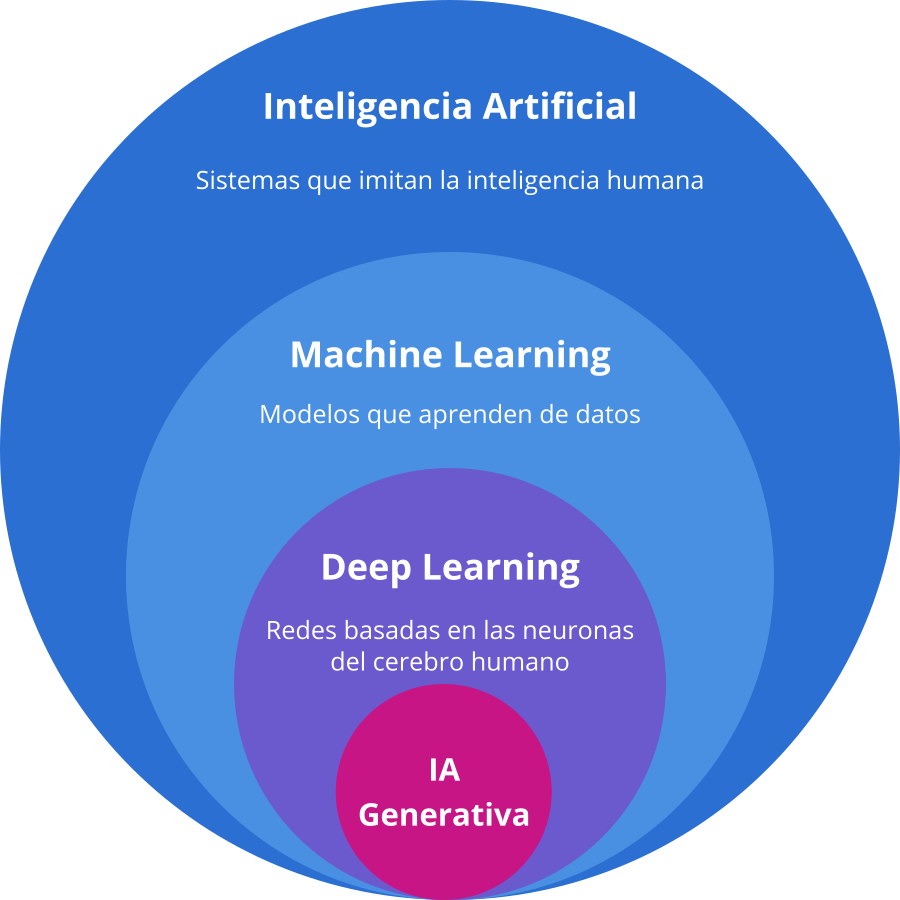
\includegraphics[width=0.6\textwidth]{figures/ia_jerarquica.png}    
    \caption{\label{fig:ia-ml-dl-gen} Relación entre IA, ML, DL e IA generativa. De creación propia.}
\end{figure}


Este TFG se centra en el Aprendizaje Profundo y el PLN, áreas dentro del Aprendizaje Automático, que como como su propio nombre indica, consisten en que el modelo \textit{aprende}, infiriendo conclusiones de datos que se le muestran. El Deep Learning se basa en el uso de redes neuronales artificiales para aprender patrones y relaciones complejas.

\section{Aprendizaje profundo y redes neuronales}
\label{redes-neuronales}

Las \textbf{redes neuronales artificiales} son algoritmos inspirados en el comportamiento de las neuronas humanas. Cada neurona artificial realiza una operación similar a una regresión lineal, combinando las entradas mediante una suma ponderada y añadiendo un \textit{sesgo}. Sin embargo, una combinación de regresiones lineales sigue siendo equivalente a otra regresión lineal, por lo que se introducen funciones de activación no lineales —como la sigmoide o la ReLU— que permiten a la red modelar relaciones más complejas.

Para entrenar estas redes se utiliza el algoritmo de \textbf{retropropagación del gradiente (backpropagation)}. Este método calcula el error de salida de la red y lo propaga hacia atrás capa por capa, ajustando los pesos mediante descenso del gradiente. En cada iteración, los parámetros se modifican en la dirección que minimiza la función de pérdida, permitiendo que la red aprenda progresivamente a realizar la tarea deseada.


\section{Arquitectura Transformer}
\label{transformers}

\subsection{Arquitectura general del Transformer}

Las arquitecturas previas de redes neuronales presentaban limitaciones a la hora de generar texto coherente y de manejar dependencias largas dentro de una secuencia. Para superar estos problemas, en 2017 se presentó la arquitectura \textbf{Transformer}, descrita en el artículo \textit{Attention is All You Need} \cite{vaswani2023attentionneed}. Esta arquitectura introdujo un cambio fundamental en el procesamiento del lenguaje natural.

El Transformer está organizado en dos bloques principales:

\begin{itemize}
    \item \textbf{Encoder}: procesa la secuencia de entrada y genera representaciones contextuales.
    \item \textbf{Decoder}: genera la salida token a token, utilizando tanto la información previa generada como la del encoder.
\end{itemize}

Cada bloque está compuesto por varias capas que combinan tres elementos fundamentales:

\begin{itemize}
    \item \textbf{Capas de atención}, que permiten al modelo identificar qué partes de la secuencia son relevantes en cada momento.
    \item \textbf{Capas de normalización}, que estabilizan el entrenamiento y evitan problemas en la retropropagación.
    \item \textbf{Capas \textit{Feed Forward}}, que son redes neuronales aplicadas de manera independiente a cada token (véase Sección \ref{redes-neuronales}).
\end{itemize}

En la Figura \ref{fig:estructura-transformers} se muestra la arquitectura original propuesta en \cite{vaswani2023attentionneed}.

\begin{figure}[H]
    \centering
    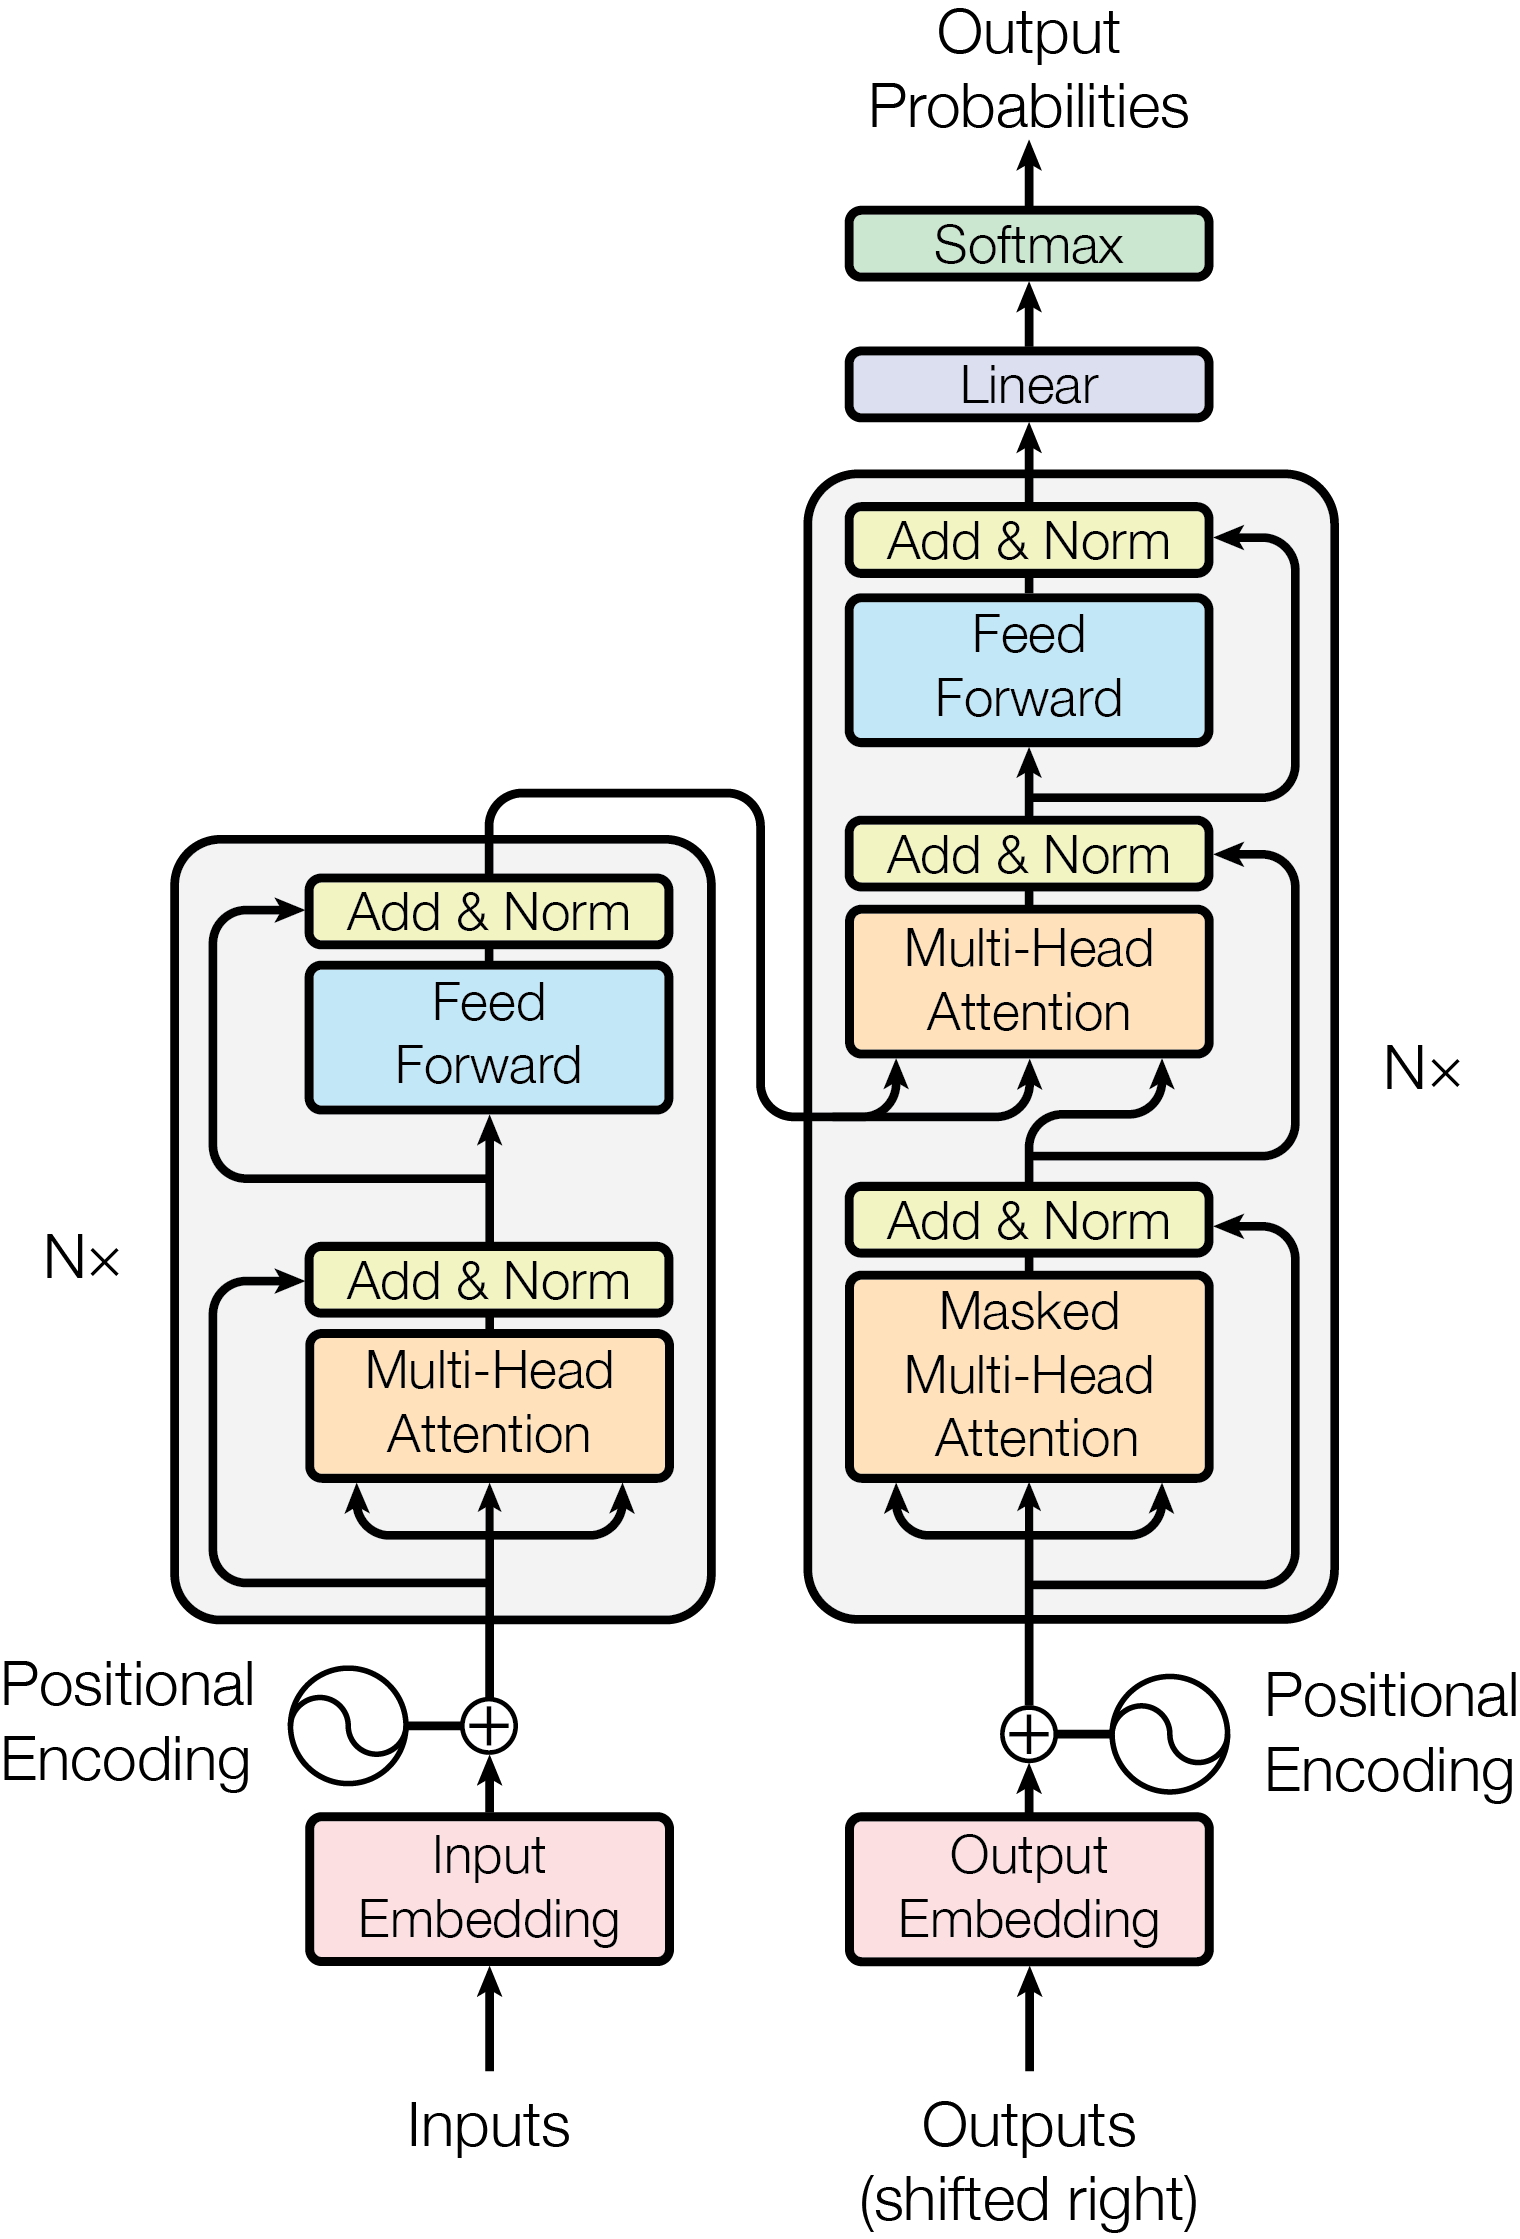
\includegraphics[width=0.5\textwidth]{figures/AttentionIsAllYouNeed.png}    
    \caption{\label{fig:estructura-transformers} Esquema de la arquitectura de un transformer \cite{vaswani2023attentionneed}.}
\end{figure}


\subsection{El mecanismo de atención}

El componente más innovador del Transformer es el mecanismo de \textbf{atención}. Este mecanismo permite procesar secuencias completas en paralelo y determinar qué partes de la entrada son más relevantes en cada contexto, algo que las arquitecturas anteriores no podían hacer de manera eficiente. La idea central es que cada token de la secuencia pueda “mirar” al resto de tokens y decidir, mediante un cálculo numérico, cuáles contienen información útil para interpretar su significado.

Para ello utiliza tres matrices fundamentales: \textbf{Query (Q)}, \textbf{Key (K)} y \textbf{Value (V)}. Cada token se proyecta en estas tres representaciones, y el modelo compara las Query con las Key para obtener una medida de similitud. Cuanto mayor es esta similitud, mayor es la atención que se asigna al token correspondiente. Esa atención se utiliza después para combinar las Value y generar una representación contextualizada, que ya no depende únicamente del token aislado, sino de su relación con el resto de la secuencia.

Este proceso permite capturar dependencias largas, como referencias a palabras que aparecen muchas posiciones antes, y también relaciones más sutiles, como concordancias gramaticales o estructuras sintácticas complejas. Además, el Transformer no se limita a una única atención, sino que utiliza varias en paralelo, conocidas como \textit{multi-head attention}. Cada cabeza aprende a fijarse en un tipo distinto de relación. Algunas detectan estructura sintáctica, otras relaciones semánticas y otras patrones más abstractos. La combinación de todas ellas produce una representación rica y expresiva del texto.

Gracias a este mecanismo, el modelo puede comprender mejor el contexto global de la secuencia y generar representaciones mucho más precisas que las obtenidas con arquitecturas recurrentes o convolucionales. La atención es, por tanto, el núcleo que permite a los Transformers escalar a grandes cantidades de datos y alcanzar el rendimiento que caracteriza a los modelos actuales.


\subsection{Inferencia y generación de texto}

El proceso de generación en un Transformer se realiza \textbf{token a token}. La salida del modelo es un vector del tamaño del vocabulario, donde cada posición representa la probabilidad de que ese token sea el siguiente. Para generar secuencias más largas, se calcula la probabilidad del siguiente token. Después se selecciona el token más probable (añadiendo aleatoriedad, para que el modelo suene más natural, llamada temperatura) y ese token se reintroduce al final del texto anterior como entrada del modelo. El proceso se repite hasta alcanzar la longitud deseada o un token de parada.

Este procedimiento permite generar texto coherente y contextualizado, aunque también introduce desafíos como la acumulación de errores o la pérdida de coherencia en secuencias largas.


\subsection{Variantes del Transformer}

El Transformer puede utilizarse de distintas maneras, dependiendo de los bloques que se utilicen:

\begin{itemize}
    \item \textbf{Encoder–Decoder} \cite{vaswani2023attentionneed}: Cogiendo el transformer completo, utilizado en tareas como la traducción automática.
    \item \textbf{Solo Encoder} \cite{devlin2019bert}: Genera representaciones semánticas numéricas de textos (por ejemplo, BERT).
    \item \textbf{Solo Decoder} \cite{brown2020language}: Arquitectura más utilizada para generación de texto, empleada por modelos como GPT, LLaMA o Qwen.
\end{itemize}

Los modelos utilizados en este proyecto pertenecen a esta última categoría, ya que están diseñados específicamente para la generación de texto.

\subsection{Impacto en los modelos de lenguaje}

La introducción de esta arquitectura supuso un salto cualitativo en tareas como la generación de texto, la traducción automática y el procesamiento del lenguaje natural en general. Gracias a los Transformers fue posible desarrollar modelos cada vez más grandes y sofisticados, dando lugar a los actuales \textbf{modelos de lenguaje de gran tamaño (LLM)}, capaces de producir resultados de alta calidad en aplicaciones como ChatGPT \cite{vaswani2023attentionneed}.


\section{Modelos de Lenguaje de Gran Tamaño (Large Language Models, LLM)}

Los LLM son arquitecturas basadas en los Transformers que, entrenadas con enormes cantidades de datos, pueden generar y comprender texto, imágenes o sonido. Entre los LLM más conocidos actualmente se encuentran GPT de OpenAI, Gemini de Google o DeepSeek, de código abierto. Estos modelos presentan varios problemas, como los sesgos derivados de los datos con los que fueron entrenados y que, en consecuencia, pueden reproducir. Además, sufren de alucinaciones, es decir, generan información inventada o sin fundamento. Sin embargo, el problema en el que se enfoca este trabajo es otro. Al necesitar grandes cantidades de datos para ser entrenados, los modelos aprenden principalmente de lenguas con abundantes recursos disponibles en internet. La principal lengua con la que se han entrenado es el inglés, lo que genera desigualdad y deja en riesgo de invisibilización a las lenguas minoritarias.

\section{Fine tuning eficiente en LLM}

Entrenar un LLM desde cero es una tarea que muy pocas instituciones o empresas pueden realizar, ya que requiere un cómputo extremadamente alto. Por eso, este trabajo se basa en una estrategia común para mejorar el rendimiento de los LLM, en vez de reentrenarlos completamente, se utiliza la técnica de \textbf{Ajuste Eficiente de Parámetros (Parameter Efficient Fine Tuning, PEFT)}. La técnica de PEFT más utilizada es \textbf{Low-Rank Adaptation (LoRA)}. La idea de LoRA consiste en añadir al peso original, de ciertas capas del transformer, una modificación entrenable de bajo rango \cite{gang:hal-04983079}. Suponiendo que una capa de la red tiene una matriz de pesos de tamaño \(N \times M\), con \(N \cdot M\) parámetros. En lugar de ajustar todos ellos, LoRA introduce dos matrices de rango reducido: 



\[
A \in \mathbb{R}^{N \times r}, \quad B \in \mathbb{R}^{r \times M}
\]



de tal manera que su producto \(A \cdot B\) genera una actualización de tamaño \(N \times M\). El número de parámetros entrenables pasa de \(N \cdot M\) a \(r \cdot (N + M)\), lo que supone un ahorro muy significativo.

Por ejemplo, si una capa tiene una matriz de pesos de tamaño \(4096 \times 4096\), el número de parámetros originales es:



\[
4096 \cdot 4096 = 16{.}777{,}216
\]



Si aplicamos LoRA con un rango reducido \(r = 8\), las dos matrices entrenables tienen:



\[
4096 \cdot 8 + 8 \cdot 4096 = 65{,}536
\]



Esto significa que en lugar de entrenar más de 16 millones de parámetros, solo se entrenarían unos 65 mil, lo que supone un ahorro superior al 99.6\% de los valores. Gracias a esta reducción, LoRA permite adaptar modelos muy grandes a nuevas tareas o lenguas con recursos limitados de manera práctica y eficiente.

Además de LoRA, en los últimos años ha surgido una variante especialmente útil en contextos con recursos limitados, \textbf{QLoRA}. Esta técnica combina las ventajas de LoRA con una cuantización del modelo base a 4 bits, lo que reduce drásticamente el uso de memoria sin afectar al rendimiento. QLoRA alcanza resultados equivalentes a los de LoRA tradicional incluso en modelos de gran tamaño, permitiendo realizar \textit{fine-tuning} eficiente en hardware modesto \cite{dettmers2023qlora}. Gracias a esta reducción de requisitos computacionales y a su estabilidad, QLoRA se ha convertido en una de las opciones más adecuadas para adaptar LLMs a nuevas lenguas.


\chapter{Estado del Arte}
\label{ch:soa}

La escasa representación de lenguas minoritarias en los LLMs constituye un desafío relevante, ya que genera desigualdades significativas entre idiomas con abundantes recursos y aquellos con escasa documentación.

Por ello, han surgido múltiples iniciativas para extender el alcance de los LLMs a otras lenguas menos representadas. Entre ellas destaca el modelo multilingüe NLLB de Meta~\cite{nllb2022}, entrenado con datos de 200 lenguas, muchas de ellas con muy pocos recursos escritos. Este modelo ha demostrado un rendimiento superior al de Google Translate en promedio, superándolo por un punto en la métrica chrF++, ampliamente utilizada en traducción automática \cite{nllb2022}.

\section{Lenguas de España}

En España existen cuatro lenguas oficiales. El castellano es la única lengua oficial en todo el territorio nacional, mientras que el catalán, el euskera y el gallego son lenguas cooficiales en sus respectivas comunidades autónomas. El catalán y el euskera se consideran lenguas con altos recursos, pero el gallego, pese a ser lengua cooficial, se considera una lengua de recursos limitados en el ámbito de la traducción automática \cite{nllb2022}.

Además de las lenguas cooficiales, existen otras lenguas reconocidas y protegidas, aunque sin estatus de cooficialidad: el asturiano, el aragonés y el aranés. Estas lenguas presentan una disponibilidad de recursos aún más limitada, lo que dificulta su integración en modelos generativos actuales.

Para fomentar el desarrollo de tecnologías lingüísticas en las lenguas oficiales, el Gobierno de España ha impulsado el proyecto ALIA \cite{ALIA2025}, que tiene como objetivo la creación de modelos y datasets en todas las lenguas cooficiales. Entre sus desarrollos destaca el modelo \textit{ALIA-40B}, capaz de generar texto en las cuatro lenguas oficiales, aunque todavía no está ajustado para seguir instrucciones, por lo que tiene dificultades para mantener conversaciones o responder preguntas \cite{alia40b2025}.

Además, el colectivo SomosNLP ha desarrollado un ranking del rendimiento de los modelos generativos disponibles en el mercado en las lenguas cooficiales de España \cite{grandury2025leaderboard}.

\subsection{Situación por lengua}
\label{subsection:situacion-por-lengua}

El \textbf{catalán} es, después del castellano, la lengua con mejor cobertura en el ámbito del PLN. Casi todos los modelos comerciales hablan catalán. Además, bajo el proyecto ALIA, el Barcelona Supercomputing Center (BSC), también ha desarrollado modelos específicos para el catalán, como el \textit{salamandra-7b-instruct}, ya preparado para usar y mantener conversaciones o responder preguntas.

Para el \textbf{euskera}, existe un modelo basado en Llama-3.1, el \textit{Latxa 3.1 Instruct 70B}. Este modelo de 70 mil millones de parámetros obtiene un resultado muy similar al de GPT4-Turbo (número de parámetros desconocido), y obtiene mejor rendimiento que todo el resto de modelos de código abierto de su mismo tamaño \cite{etxaniz2024latxa}.

Por último, para el \textbf{gallego} se han entrenado modelos específicos como \textit{Carballo-cerebras-1.3B}. Este modelo ha demostrado una capacidad notable para generar texto de calidad en esta lengua, pero con capacidad de mejora en tareas como la reformulación de frases, donde obtiene peor rendimiento que modelos multilingües de su tamaño, como \textit{Bloom-1.7B} \cite{gamallo2024opengenerativelargelanguage}.

En el caso del \textbf{asturiano}, \textbf{aragonés} y \textbf{aranés}, no se han identificado modelos especializados ni para tareas de traducción ni de generación de texto.

\section{Otros modelos para lenguas minoritarias}

Dado el contexto de recursos limitados y la necesidad de eficiencia computacional, resulta útil revisar enfoques aplicados en otras lenguas de bajos recursos. Por ejemplo, en Salma Khaled et al. \cite{KHALED2025103682} se ha desarrollado un sistema de análisis de sentimiento para variantes del árabe utilizando estrategias de ajuste eficiente como LoRA (Low-Rank Adaptation). Este tipo de técnicas permite adaptar modelos grandes con un coste computacional reducido, lo que las hace especialmente adecuadas para lenguas con escasez de datos y recursos, y por tanto potencialmente replicables en el estudio de las lenguas minoritarias de España.

Otro trabajo relevante en el ámbito de las lenguas minoritarias es el estudio \textit{Open and Closed-Source LLMs for Low-Resource Languages with Zero-Shot, Few-Shot, and Chain-of-Thought Prompting}. En este análisis, los autores comparan modelos abiertos y propietarios en múltiples lenguas minoritarias, evaluando su rendimiento bajo múltiples estrategias de prompting: \textit{zero-shot}, \textit{few-shot} y \textit{chain-of-thought}. El estudio demuestra que, incluso sin datos específicos de entrenamiento, los LLMs pueden ofrecer resultados razonables en lenguas de bajo recurso mediante técnicas de prompting adecuadas \cite{NAZI2025100124}. Sin embargo, también pone de manifiesto que el rendimiento mejora significativamente cuando se dispone de ejemplos en la lengua objetivo, aunque sean pocos, lo que subraya la importancia de recopilar o traducir pequeños conjuntos de datos de alta calidad. 


\section{Evaluación de LLMs}
\label{sec:Evaluacion}

La evaluación de los LLM ha evolucionado rápidamente en los últimos años, impulsada por la necesidad de medir de forma rigurosa sus capacidades en tareas diversas y en múltiples lenguas. Los primeros esfuerzos de evaluación a gran escala se centraron en lenguas de alto recurso, lo que generó marcos metodológicos sólidos pero poco representativos para lenguas minoritarias. Un ejemplo paradigmático es HELM (\textit{Holistic Evaluation of Language Models}), que propone un marco exhaustivo y estandarizado para evaluar LLMs en dimensiones como precisión, robustez, eficiencia o equidad \cite{liang2022helm}. Aunque HELM constituye un hito metodológico, su cobertura lingüística sigue siendo limitada, lo que deja fuera a la mayoría de lenguas de bajo recurso.

Otro referente es BIG-Bench \cite{srivastava2022bigbench}. Un benchmark masivo con más de 200 tareas diseñadas para explorar las capacidades emergentes de los LLMs. Sin embargo, al igual que HELM, BIG-Bench se centra casi exclusivamente en lenguas de alta disponibilidad de datos, lo que evidencia una brecha estructural, los marcos de evaluación más influyentes no contemplan lenguas como el asturiano, el aragonés, el gallego o muchas otras. Esta falta de representación lingüística limita la capacidad de estos benchmarks para ofrecer una evaluación justa y comparativa en contextos multilingües.

En el ámbito multilingüe, FLORES-200 constituye uno de los avances más significativos. Este benchmark, desarrollado en el contexto del proyecto \textit{No Language Left Behind}, permite evaluar sistemas de traducción en 200 lenguas, muchas de ellas de bajo recurso. Aunque su enfoque se centra en la traducción automática, FLORES-200 demuestra que es posible construir recursos multilingües amplios y equilibrados, y demuestra la importancia de disponer de datos paralelos de alta calidad para lenguas minoritarias \cite{nllb2022}. 

En respuesta a estas carencias, han surgido iniciativas específicas para lenguas de la península ibérica. Entre ellas destaca \textit{IberBench} \cite{gonzalez2026iberbench}, un benchmark diseñado para evaluar LLMs en lenguas iberorromances, incluyendo gallego, euskera y catalán. IberBench integra más de un centenar de datasets procedentes de campañas de evaluación previas y tareas adaptadas, abarcando clasificación, análisis de sentimiento, resumen y otras tareas de comprensión. Su principal aportación es proporcionar un marco homogéneo que permite comparar modelos abiertos y cerrados en lenguas tradicionalmente infrarepresentadas.

Por último, se ha analizado el rendimiento de modelos abiertos y propietarios en lenguas de bajo recurso bajo configuraciones \textit{zero-shot}, \textit{few-shot} y \textit{chain-of-thought}. El estudio muestra que, ante la falta de recursos lingüísticos, la comunidad recurre a dos estrategias principales. La primera es la creación manual de datasets en la lengua objetivo. La segunda es la traducción de benchmarks existentes desde lenguas de alto recurso, ya sea mediante traducción humana o automática. Ambas estrategias permiten realizar evaluaciones comparables, pero introducen limitaciones importantes, como sesgos de traducción, pérdida de matices lingüísticos y una cobertura temática reducida \cite{NAZI2025100124}.

En conjunto, estos trabajos evidencian una limitación estructural. La evaluación de LLMs en lenguas minoritarias depende de la creación manual, costosa y poco escalable de nuevos conjuntos de datos. A diferencia de las lenguas mayoritarias, que cuentan con ecosistemas de evaluación consolidados, las lenguas de bajo recurso requieren esfuerzos ad hoc para cada nueva tarea o benchmark. Esta situación subraya la necesidad de desarrollar metodologías multilingüe, que permitan evaluar modelos en un espectro amplio de lenguas sin depender de la construcción manual de datasets para cada una de ellas.
\chapter{Metodología y materiales}
\label{ch:inicioIR}

En este capítulo se exponen las fases en las que se va a realizar el estudio, los datos recopilados y el entorno experimental que se utilizan para el desarrollo del proyecto.
\section{Metodología}

La metodología seguida en este trabajo se ha diseñado para abordar de forma sistemática el estudio, adaptación y evaluación de modelos de lenguaje en lenguas minoritarias de España. El proceso es un pipeline que se estructura en cinco fases consecutivas, cada una con objetivos y actividades claramente definidos, que permiten avanzar desde la exploración inicial del estado del arte hasta la obtención de un modelo ajustado y su evaluación comparativa.

\subsection*{Fase 1: Exploración de modelos existentes}
En esta primera fase se analizan los modelos de lenguaje disponibles que puedan servir como punto de partida para el estudio. Se revisan sus arquitecturas, tamaños, capacidades multilingües y rendimiento en las lenguas cooficiales, apoyándose en recursos como la \textit{leaderboard} de SomosNLP. El objetivo es identificar modelos representativos en distintos rangos de parámetros y con enfoques arquitectónicos diversos, que permitan comprender las limitaciones actuales en lenguas de bajo recurso.

\subsection*{Fase 2: Definición de métricas y tareas de evaluación}
Una vez identificados los modelos candidatos, se diseña un conjunto de métricas y tareas que permitan evaluar su rendimiento de forma homogénea. Se seleccionan tareas relevantes para lenguas minoritarias, como traducción, corrección gramatical o análisis de interferencias lingüísticas. Para cada tarea se establecen métricas cuantitativas (BLEU, chrF++, tasas de error) y criterios cualitativos, garantizando una evaluación reproducible y comparable entre modelos.

\subsection*{Fase 3: Selección y preparación del modelo a adaptar}
Tras la evaluación preliminar, se selecciona el modelo más adecuado para ser adaptado mediante técnicas de \textit{fine-tuning} eficiente. En esta fase se realiza la preparación del modelo base, la configuración de los parámetros de entrenamiento, la integración del QLoRA y la configuración de los hiperparámetros. Asimismo, se lleva a cabo la limpieza, normalización y alineación de los conjuntos de datos necesarios para el entrenamiento del modelo en las lenguas objetivo.

\subsection*{Fase 4: Entrenamiento y análisis del modelo adaptado}
En esta fase se entrena el modelo seleccionado utilizando los datos preparados y la configuración definida. Se monitoriza el proceso de entrenamiento, analizando la estabilidad, la convergencia y el impacto del QLoRA. Además, se documentan las decisiones tomadas durante el proceso y se evalúan los primeros resultados para detectar posibles problemas o mejoras necesarias.

\subsection*{Fase 5: Evaluación final y comparativa}
Finalmente, el modelo adaptado se evalúa utilizando las métricas y tareas definidas en la Fase 2. Se comparan sus resultados con los obtenidos por los modelos analizados en la Fase 1, permitiendo determinar si la adaptación ha mejorado el rendimiento en las lenguas minoritarias. Esta fase incluye tanto un análisis cuantitativo como cualitativo, así como una discusión de las limitaciones y del impacto real de la adaptación realizada.
\\
\\
Un gráfico que muestra la metodología seguida y su flujo secuencial, se puede observar en la Figura \ref{fig:metodologia-trabajo}.

\begin{figure}[H]
    \centering
    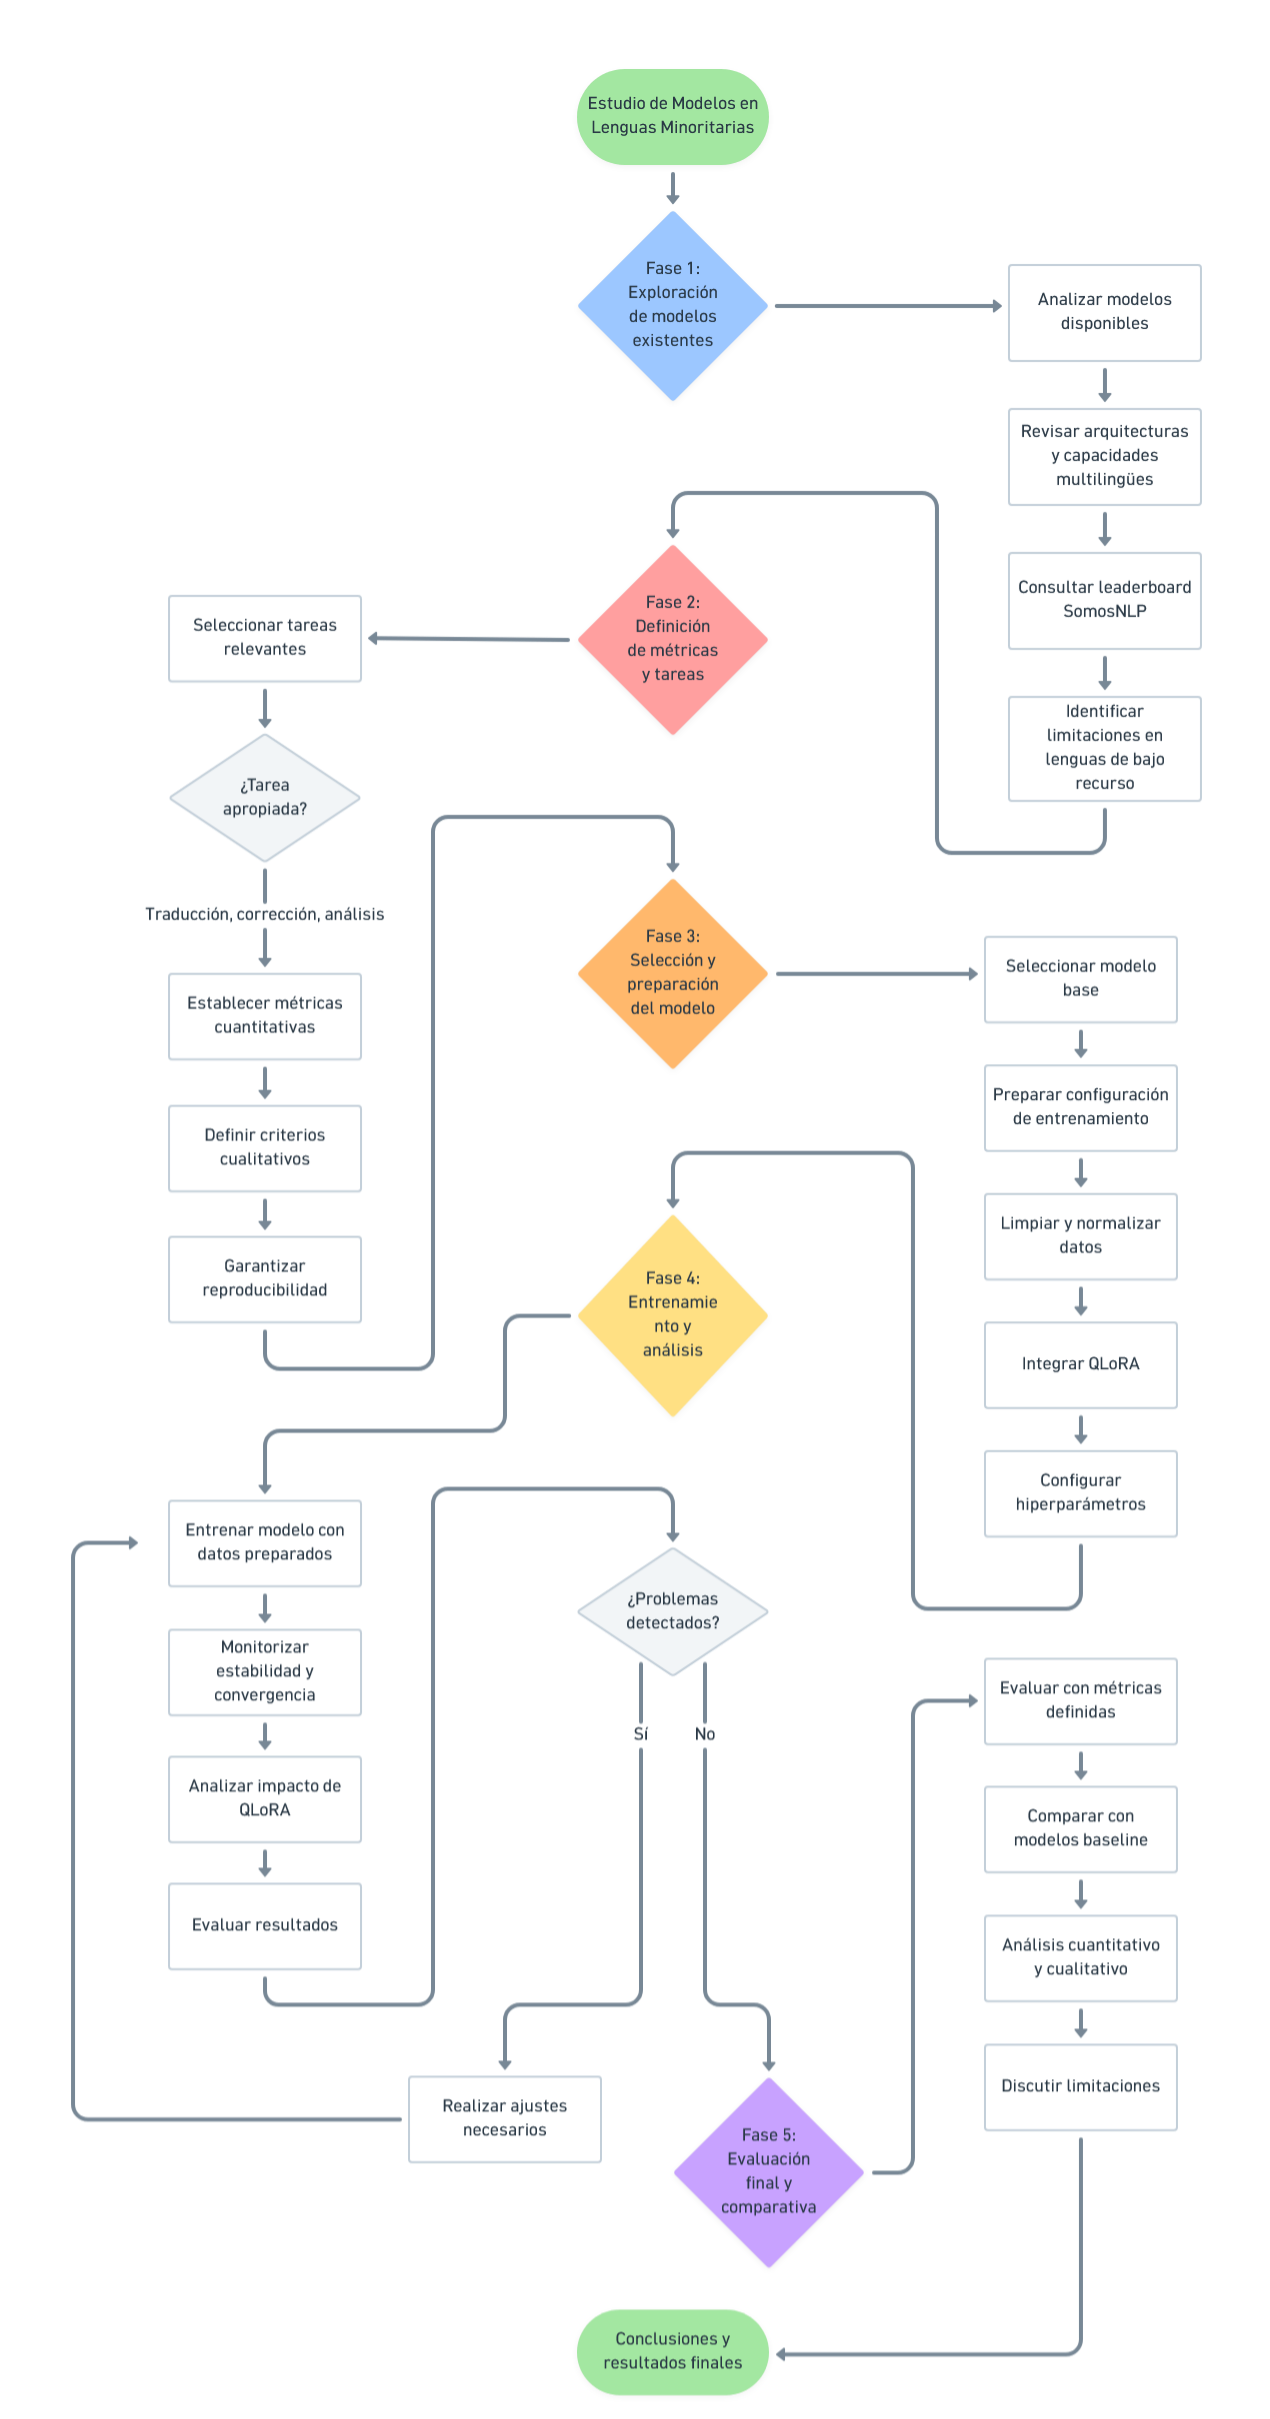
\includegraphics[width=0.8\textwidth]{figures/MetodologíaV2.png}    
    \caption{\label{fig:metodologia-trabajo} Resumen visual de la metodología empleada. De creación propia.}
\end{figure}


\section{Materiales}

\subsection{Conjuntos de datos}
\label{conjuntos-de-datos}
\subsubsection{Proceso de exploración}
Se ha comenzado revisando los datasets utilizados por Alia, analizando los idiomas que incluyen y el número de frases disponibles en cada uno. 
Posteriormente se han buscado otras fuentes de datos, entre las cuales destaca OPUS, que es especialmente grande. 

Todas estas fuentes permiten descargar y utilizar los datos con facilidad, aunque algunos corpus son muy voluminosos, quizá demasiado para ciertos usos.

\subsubsection{Datasets previamente encontrados}

Alia, la infraestructura pública de IA en castellano y lenguas cooficiales, ofrece conjuntos de datos de texto, voz y traducción automática. Es un recurso útil tanto para obtener datos como para comparar resultados \cite{ALIA2025}.

Otra gran plataforma donde se pueden encontrar varios conjuntos de datos es \textbf{OPUS}. OPUS reúne y distribuye corpus paralelos multilingües de acceso abierto. Su objetivo es facilitar la investigación en traducción automática, alineación de textos y aprendizaje de modelos multilingües. Los datos provienen de múltiples fuentes (como subtítulos, documentos oficiales o la Wikipedia). Se utilizarán los datos de esta web para el asturiano y el aranés, que no cuentan con un conjunto de datos grande ya creado \cite{tiedemann-2012-parallel}.

Para el \textbf{gallego} se encontró un dataset de más de 2 mil millones de palabras. Este corpus se nutre de libros, enciclopedias, datos gubernamentales, prensa, artículos de investigación, webs públicas, Wikipedia, corpus de traducción y otros web crawls \cite{CorpusNOS-GL}.

Por otro lado, se encuentra el proyecto LiLowLa \cite{LiLowLa2022} de la Universidad de Alicante. El objetivo de este proyecto \textit{(Lightweight neural translation technologies for low-resource languages)} es mejorar el rendimiento de la traducción automática neuronal y de las memorias de traducción en pares de lenguas con escasos recursos. Incluye un dataset con texto en aragonés, aranés, asturiano y valenciano \cite{perez-ortiz-etal-2024-expanding}.

También se incluirán los datos de \textbf{Tatoeba}. Aunque el número de frases en asturiano y aranés es reducido, resulta una fuente útil para ampliar la cobertura y enriquecer los conjuntos de datos ya mencionados \cite{Tatoeba2025}.

Finalmente, se pueden extraer más datos aplicando técnicas de \textit{web scraping} en páginas dedicadas a las propias lenguas. Para el \textbf{asturiano}, existen recursos como la Academia de la Llingua Asturiana, con artículos y textos en asturiano, además de documentos en PDF como la gramática \cite{ALLA2024}, o Eslema, una página con corpus en asturiano \cite{Viejo2008}. Para el \textbf{aranés} se dispone del Institut d'Estudis Aranesi \cite{InstitutEstudisAranesi2014}, con documentos tan útiles como la \textit{Gramática del Aranés} \cite{GramaticaAranes2021}.

Todos los datos recopilados se procesan y limpian como se describe en la sección 6.1, \nameref{sec:Limpieza}. Después de limpiarlos se han publicado en HuggingFace con todo el material del TFG \url{https://hf.co/collections/MiguelGP-13/tfg} \cite{lexicons_2025, galician_instructive_2025, asturian_instructive_2025, aranes_instructive_2025, asturian_annotated_2025, galician_annotated_2025, aranes_annotated_2025, asturian_cloze_2025, galician_cloze_2025, aranes_cloze_2025}.


\section{Setup}

El trabajo se ha desarrollado principalmente en entornos de ejecución en la nube, por lo que no se ha requerido hardware local especializado. Para la experimentación y generación de resultados se ha utilizado:

\begin{itemize}
    \item \textbf{Gradient PaperSpace}, que proporciona acceso a una GPU NVIDIA RTX5000, con 16 GB de VRAM, y 30 GB de memoria RAM del sistema. Este entorno se ha empleado para la ejecución de código en Python para el entrenamiento y la evaluación de los modelos.
    \item \textbf{Equipo local} que se ha utilizado para tareas auxiliares, como edición de figuras, pruebas y revisión de código, sin requerimientos de hardware específicos.
\end{itemize}

Este conjunto de recursos resulta suficiente para la experimentación con modelos de tamaño medio. Para el uso de modelos más grandes, se ha usado la API de Groq.

\section{Marco Tecnológico}

El desarrollo del proyecto ha requerido un conjunto de herramientas y tecnologías que permiten la ejecución de experimentos, la evaluación de modelos y la elaboración de la memoria. Las principales herramientas empleadas han sido:

\begin{itemize}
    \item \textbf{Python 3.12} como lenguaje principal para la implementación del benchmark y la manipulación de datos \cite{python}.
    \item \textbf{Groq API}, utilizada para la inferencia con modelos de gran tamaño (GPT-oss 120B), empleado como modelo evaluador en el benchmark \cite{groqapi}.
    \item \textbf{Bibliotecas de Python} relevantes para el procesamiento, entrenamiento y análisis, entre ellas:
    \begin{itemize}
        \item \texttt{transformers} para la interacción con modelos de lenguaje y su ajuste fino \cite{wolf2020transformers}.
        \item \texttt{datasets} para la gestión de corpus y datos experimentales \cite{lhoest2021datasets}.
        \item \texttt{accelerate} para la ejecución eficiente en GPU y CPU distribuidas \cite{accelerate}.
        \item \texttt{bitsandbytes} para la cuantización y optimización de modelos de gran tamaño \cite{bitsandbytes}.
        \item \texttt{peft} para la aplicación de técnicas de ajuste fino eficiente como LoRA \cite{peft}.
        \item \texttt{pandas} y \texttt{numpy} para el procesamiento y análisis de datos \cite{pandas,numpy}.
        \item \texttt{scikit-learn} para métricas y análisis estadístico \cite{scikit-learn}.
        \item \texttt{python-dotenv} para la gestión de claves y variables de entorno \cite{python-dotenv}.
        \item \texttt{lowresource-llm-evaluation} código creado en este proyecto, disponible a través de pip (\textit{\url{https://pypi.org/project/lowresource-llm-evaluation/}}), incluyendo el benchmark, una clase para gestionar y limpiar los datos y funciones auxiliares como las de creación de los datasets necesarios para el benchmark o analizar los resultados.
    \end{itemize}
    \item \textbf{Overleaf} para la redacción de la memoria en \LaTeX.
    \item \textbf{Inkscape}, \textbf{Whismical} y \textbf{GIMP} para la creación y edición de figuras y diagramas.
    \item \textbf{Visual Studio Code} como entorno de desarrollo para la implementación de scripts y generación de datasets.
\end{itemize}

Este conjunto de herramientas proporciona un entorno completo y reproducible para el desarrollo del benchmark y la elaboración del trabajo. Todo el código del TFG se encuentra disponible en el siguiente repositorio de GitHub: \url{https://github.com/MiguelGP-13/TFG}.

\chapter{Fase 1: Análisis Exploratorio de Modelos y Métodos de Adaptación}
\label{ch:extraccion}

En esta fase se examina el estado actual de los modelos de lenguaje y las metodologías disponibles para extender sus competencias a lenguas con pocos recursos. El objetivo es identificar qué enfoques son los que mejores resultados van a aportar, teniendo en cuenta los datos y recursos de cómputo limitados del proyecto.

% hay que explicar por cada fase de la metodología lo que se ha hecho
\section{Análisis de los modelos existentes}

Para comenzar el análisis de los modelos existentes, se ha seleccionado un conjunto de modelos que permite cubrir distintos rangos de tamaño y arquitecturas, con el fin de evaluar su comportamiento en las lenguas minoritarias en España. Su elección se ha basado principalmente en el ranking en La leaderboard \cite{grandury2025leaderboard}, observando el rendimiento en las lenguas cooficiales. Se han elegido:

\subsection*{Salamandra-7B}
Salamandra-7B \cite{gonzalezagirre2025salamandratechnicalreport} se incorpora como modelo de referencia en español gracias a su entrenamiento intensivo en castellano y otras lenguas europeas, lo que le permite ofrecer una cobertura lingüística sólida y un rendimiento competitivo en tareas en español. Su principal fortaleza radica en esta especialización, que lo convierte en un punto de comparación útil para analizar el comportamiento de modelos generalistas en lenguas con recursos limitados. No obstante, su enfoque centrado en el castellano y su tamaño medio pueden traducirse en una menor robustez multilingüe y en limitaciones frente a arquitecturas más recientes optimizadas para eficiencia y razonamiento profundo.

\subsection*{Mistral-7B}
Mistral-7B \cite{jiang2023mistral} representa un modelo de tamaño medio con una arquitectura especialmente eficiente, capaz de ofrecer un rendimiento por parámetro muy competitivo y una estabilidad notable en tareas generales y multilingües. Su principal fortaleza reside en esta eficiencia, que lo convierte en un punto intermedio sólido para estudiar el escalado de capacidades. Sin embargo, su entrenamiento no está tan orientado a lenguas minoritarias, lo que puede generar variabilidad en escenarios con recursos lingüísticos muy limitados.

\subsection*{Qwen-2.5-7B}
Qwen-2.5-7B \cite{qwen2.5_2024} se selecciona como modelo compacto que destaca por su excelente relación entre tamaño y rendimiento, apoyado en una arquitectura moderna y un entrenamiento multilingüe amplio. Su principal fortaleza es precisamente esta eficiencia, que permite analizar cómo se comportan modelos ligeros en tareas complejas sin requerir grandes recursos computacionales. Aun así, su menor capacidad puede traducirse en limitaciones en razonamiento profundo, consistencia en tareas largas o robustez en lenguas con muy pocos datos.

\subsection*{Gemma-7B}
Gemma-7B \cite{gemma2024} se incorpora como modelo mediano equilibrado, caracterizado por un entrenamiento multilingüe de alta calidad y un diseño estable que facilita su uso como referencia en estudios de escalado. Su principal fortaleza es este equilibrio entre eficiencia y capacidad, que lo convierte en un punto intermedio adecuado entre modelos pequeños y grandes. No obstante, su rendimiento en lenguas extremadamente minoritarias o en tareas muy especializadas puede ser menos competitivo que el de modelos de mayor tamaño o con corpus más diversificados.


\section{Identificación de las posibles soluciones}
% Comparativa de opciones técnicas y estrategias
El objetivo de este TFG es obtener un modelo de lenguaje para cada una de las lenguas estudiadas, capaz de utilizarlas con la mayor fluidez y precisión posible. Para ello, es necesario analizar qué estrategias existen actualmente para dotar a un LLM de nuevas competencias, siguiendo prácticas habituales en el desarrollo y adaptación de modelos multilingües. 


\begin{enumerate}
\item \textbf{Entrenamiento de un modelo desde cero} 

La primera opción sería entrenar un modelo desde cero, utilizando texto en estas lenguas y complementándolo con texto en otras lenguas mayoritarias para disponer de suficientes datos de entrenamiento. GPT‑2, uno de los primeros LLM cuyo rendimiento se aproximaba al de un humano, se entrenó con 40 GB de texto extraído de internet \cite{radford2019language}. Este volumen de entrenamiento es inabarcable con los recursos disponibles y, además, supondría un gasto innecesario.

Actualmente existen modelos de gran calidad, muchos de ellos multilingües. Resulta mucho más eficiente enseñar a esos modelos las lenguas en las que nos enfocamos, aprovechando su conocimiento previo y su capacidad de generar texto.

\item \textbf{Reentrenamiento de modelos existentes}

Viendo inviable e innecesario el entrenamiento de un modelo nuevo, se podría reentrenar un modelo existente, con texto en las lenguas de estudio, de modo que el sistema aprendiera a generar y comprender asturiano, aranés o gallego a partir de ejemplos directos. Esta idea evita el enorme coste computacional de entrenar un modelo desde cero y aprovecha el conocimiento lingüístico general que los LLM ya poseen. Además, existen técnicas como dejar ciertas capas profundas congeladas que permitirían reducir el número de parámetros actualizables, haciendo el proceso más manejable.

Sin embargo, este enfoque presenta limitaciones importantes. La más conocida es el \textit{catastrophic forgetting}, un fenómeno ampliamente documentado en redes neuronales. Cuando un modelo se ajusta a una nueva tarea, puede perder parte de lo aprendido previamente si los parámetros relevantes se modifican en exceso durante el reentrenamiento \cite{Kirkpatrick_2017}. En el contexto de los modelos de lenguaje modernos, se ha comprobado empíricamente que este fenómeno degrada drásticamente las capacidades generales del modelo tras un ajuste fino continuo \cite{luo2023an}. Esto significa en nuestro caso, que un modelo adaptado para mejorar su rendimiento en una lengua minoritaria podría deteriorar su rendimiento en tareas previamente aprendidas. Este riesgo es especialmente relevante en ámbitos donde los corpus disponibles son pequeños y no permiten un ajuste estable. A ello se suma que el \textit{fine-tuning} completo sigue requiriendo grandes recursos computacionales y un control cuidadoso para evitar sobreajuste. Por estas razones, aunque el reentrenamiento total es conceptualmente sencillo, no parece ser la opción más adecuada para este proyecto.

\item \textbf{Adaptación de modelos existentes}

Ante las limitaciones del reentrenamiento completo, la comunidad científica ha desarrollado métodos de adaptación más eficientes, conocidos como \textit{Parameter-Efficient Fine-Tuning} (PEFT). Estos enfoques buscan modificar únicamente una pequeña parte del modelo, manteniendo congelados la mayoría de sus parámetros. Entre las primeras propuestas destacadas se encuentran los \textit{adapters} \cite{houlsby2019parameterefficienttransferlearningnlp}. Su idea consiste en insertar módulos adicionales de reducido tamaño entre las capas del transformador, de modo que solo estos módulos se entrenan mientras el resto del modelo permanece intacto. Este diseño permite adaptar el modelo a nuevas tareas o lenguas sin alterar su conocimiento previo, reduciendo así el riesgo de \textit{catastrophic forgetting}. Posteriormente, se amplió este enfoque con \textit{AdapterFusion}, que permite combinar varios adapters entrenados en distintos dominios o lenguas sin necesidad de reentrenarlos conjuntamente, demostrando la flexibilidad de esta familia de métodos \cite{pfeiffer2021adapterfusionnondestructivetaskcomposition}.

A pesar de su utilidad, los adapters presentan ciertas limitaciones prácticas. Requieren modificar la arquitectura interna del modelo, añadiendo módulos en cada capa, y su rendimiento depende de la compatibilidad con la estructura del transformer original. Para superar estas restricciones surgieron métodos más recientes como LoRA (\textit{Low-Rank Adaptation}) \cite{hu2021loralowrankadaptationlarge}. Esta técnica reduce drásticamente el número de parámetros entrenables y evita los problemas de compatibilidad arquitectónica propios de los adapters tradicionales. Además, su variante QLoRA permite entrenar modelos grandes en hardware modesto mediante cuantización de 4 bits, manteniendo un rendimiento competitivo \cite{dettmers2023qlora}.

En conjunto, los métodos PEFT ofrecen una alternativa mucho más adecuada que el \textit{fine-tuning} completo para lenguas minoritarias. Los adapters aportan modularidad y reutilización, mientras que LoRA y QLoRA destacan por su eficiencia, simplicidad y bajo coste computacional. 

Considerando las limitaciones de datos y recursos de este proyecto, la opción más razonable es emplear LoRA o QLoRA, ya que permiten adaptar el modelo a las lenguas objetivo sin comprometer su rendimiento general ni incurrir en los riesgos asociados al reentrenamiento completo.


\end{enumerate}


\section{Evaluación de la solución seleccionada}

Tras comparar las distintas alternativas, la solución que se va a implementar es QLoRA. Las técnicas de \textit{fine-tuning} completo quedan descartadas por su elevado coste computacional y por el riesgo de \textit{catastrophic forgetting}, el cual resulta especialmente crítico al adaptar LLMs mediante actualizaciones completas de sus parámetros \cite{luo2023an}, mientras que los métodos PEFT ofrecen una adaptación mucho más eficiente y segura. Dentro de ellos, QLoRA resulta especialmente ventajoso porque permite ajustar modelos de gran tamaño en hardware limitado gracias a la cuantización en 4 bits, manteniendo un rendimiento equivalente al de LoRA tradicional \cite{dettmers2023qlora}. Esta eficiencia es determinante en un contexto como el de este proyecto, donde los recursos son reducidos y los corpus son pequeños. Además, QLoRA, al igual que LoRA, conserva intactos los parámetros originales del modelo, lo que minimiza la pérdida de conocimiento previo y facilita la reproducibilidad. Por todo ello, QLoRA proporciona el mejor equilibrio entre coste, estabilidad y calidad para adaptar un modelo multilingüe a las lenguas estudiadas.


\chapter{Fase 2: Desarrollo del método de entrenamiento del LLM}
\label{ch:analisis}


El entrenamiento de un LLM requiere establecer, desde el inicio, una base metodológica sólida. Antes de cualquier fase de entrenamiento, resulta fundamental determinar qué datos se emplearán, cómo serán limpiados, homogeneizados y filtrados, y en qué componentes del modelo se aplicarán las técnicas de adaptación eficiente como QLoRA. Estas decisiones iniciales condicionan de manera directa la calidad del modelo resultante, ya que definen el tipo de información lingüística que podrá aprender y la forma en que sus parámetros serán ajustados.

Una vez fijado este marco, se procede a la configuración de los hiperparámetros. Durante el entrenamiento pueden ajustarse progresivamente para mejorar la estabilidad o la convergencia, pero su impacto es limitado si los datos no han sido preparados adecuadamente. 


\section{Limpieza y preparación de los datos}
\label{sec:Limpieza}

Para gestionar de forma unificada los distintos corpus utilizados en este trabajo, se desarrolló una clase propia denominada \texttt{LanguageDatasets}. Esta clase actúa como un contenedor estructurado que centraliza la descarga, lectura, limpieza y almacenamiento de los datos. Cada instancia mantiene un registro de los fragmentos pertenecientes a cada fuente, permite acceder a ellos tanto por índice como por nombre del dataset y ofrece utilidades adicionales como la conversión directa a un \textit{Dataset} de HuggingFace o la tokenización mediante cualquier tokenizer externo. De este modo, se garantiza un flujo de trabajo reproducible, modular y fácilmente extensible para cada una de las lenguas analizadas.

Una vez recopilados los conjuntos de datos descritos en la Sección 4.2.1, se aplicó un proceso de limpieza diseñado para eliminar ruido, unificar formatos y asegurar que el corpus resultante fuera adecuado para su uso en tareas de evaluación en gallego, asturiano y aranés. Este proceso se implementó mediante una serie de transformaciones encadenadas aplicadas a cada línea de texto.

En primer lugar, se eliminaron elementos estructurales irrelevantes, tales como hashtags, etiquetas HTML y direcciones URL. También se decodificaron entidades HTML con el fin de recuperar los caracteres originales presentes en el texto. Posteriormente, se eliminaron emojis y otros símbolos no pertenecientes al alfabeto latino, manteniendo únicamente letras, números, espacios y signos de puntuación básicos, incluyendo apóstrofos y guiones, que son frecuentes en lenguas como el asturiano o el aranés.

Para garantizar la coherencia interna del corpus, se aplicó una normalización Unicode en formato NFC, lo que permite unificar caracteres equivalentes que pueden aparecer representados de forma distinta según la fuente (por ejemplo, vocales acentuadas compuestas frente a caracteres precompuestos). A continuación, se normalizaron los espacios en blanco y se limitaron repeticiones excesivas tanto de caracteres como de palabras, sustituyendo secuencias de más de cinco repeticiones por una versión acotada.

Por último, se aplicaron filtros destinados a descartar textos de baja calidad: líneas demasiado cortas, secuencias dominadas por una única palabra, fragmentos con palabras anormalmente largas o textos con un porcentaje elevado de palabras de un solo carácter. También se estableció un límite máximo de longitud para evitar la inclusión de fragmentos desproporcionadamente extensos. Durante este proceso se revisaron manualmente ejemplos de frases que superaban la limpieza inicial y se observó que, aun siendo técnicamente válidas, muchas de ellas no aportaban información lingüística útil para la evaluación. Por este motivo se añadieron criterios adicionales de filtrado orientados a eliminar contenido redundante, trivial o carente de estructura. Cada línea que superó estos filtros se almacenó en el formato \texttt{\{"text": frase\}}, compatible con las herramientas de HuggingFace y fácilmente extensible para añadir metadatos adicionales en el futuro. Un ejemplo de la limpieza se puede ver en la Figura \ref{fig:ejemplo-limpieza}.


\begin{figure}[H]
    \centering
    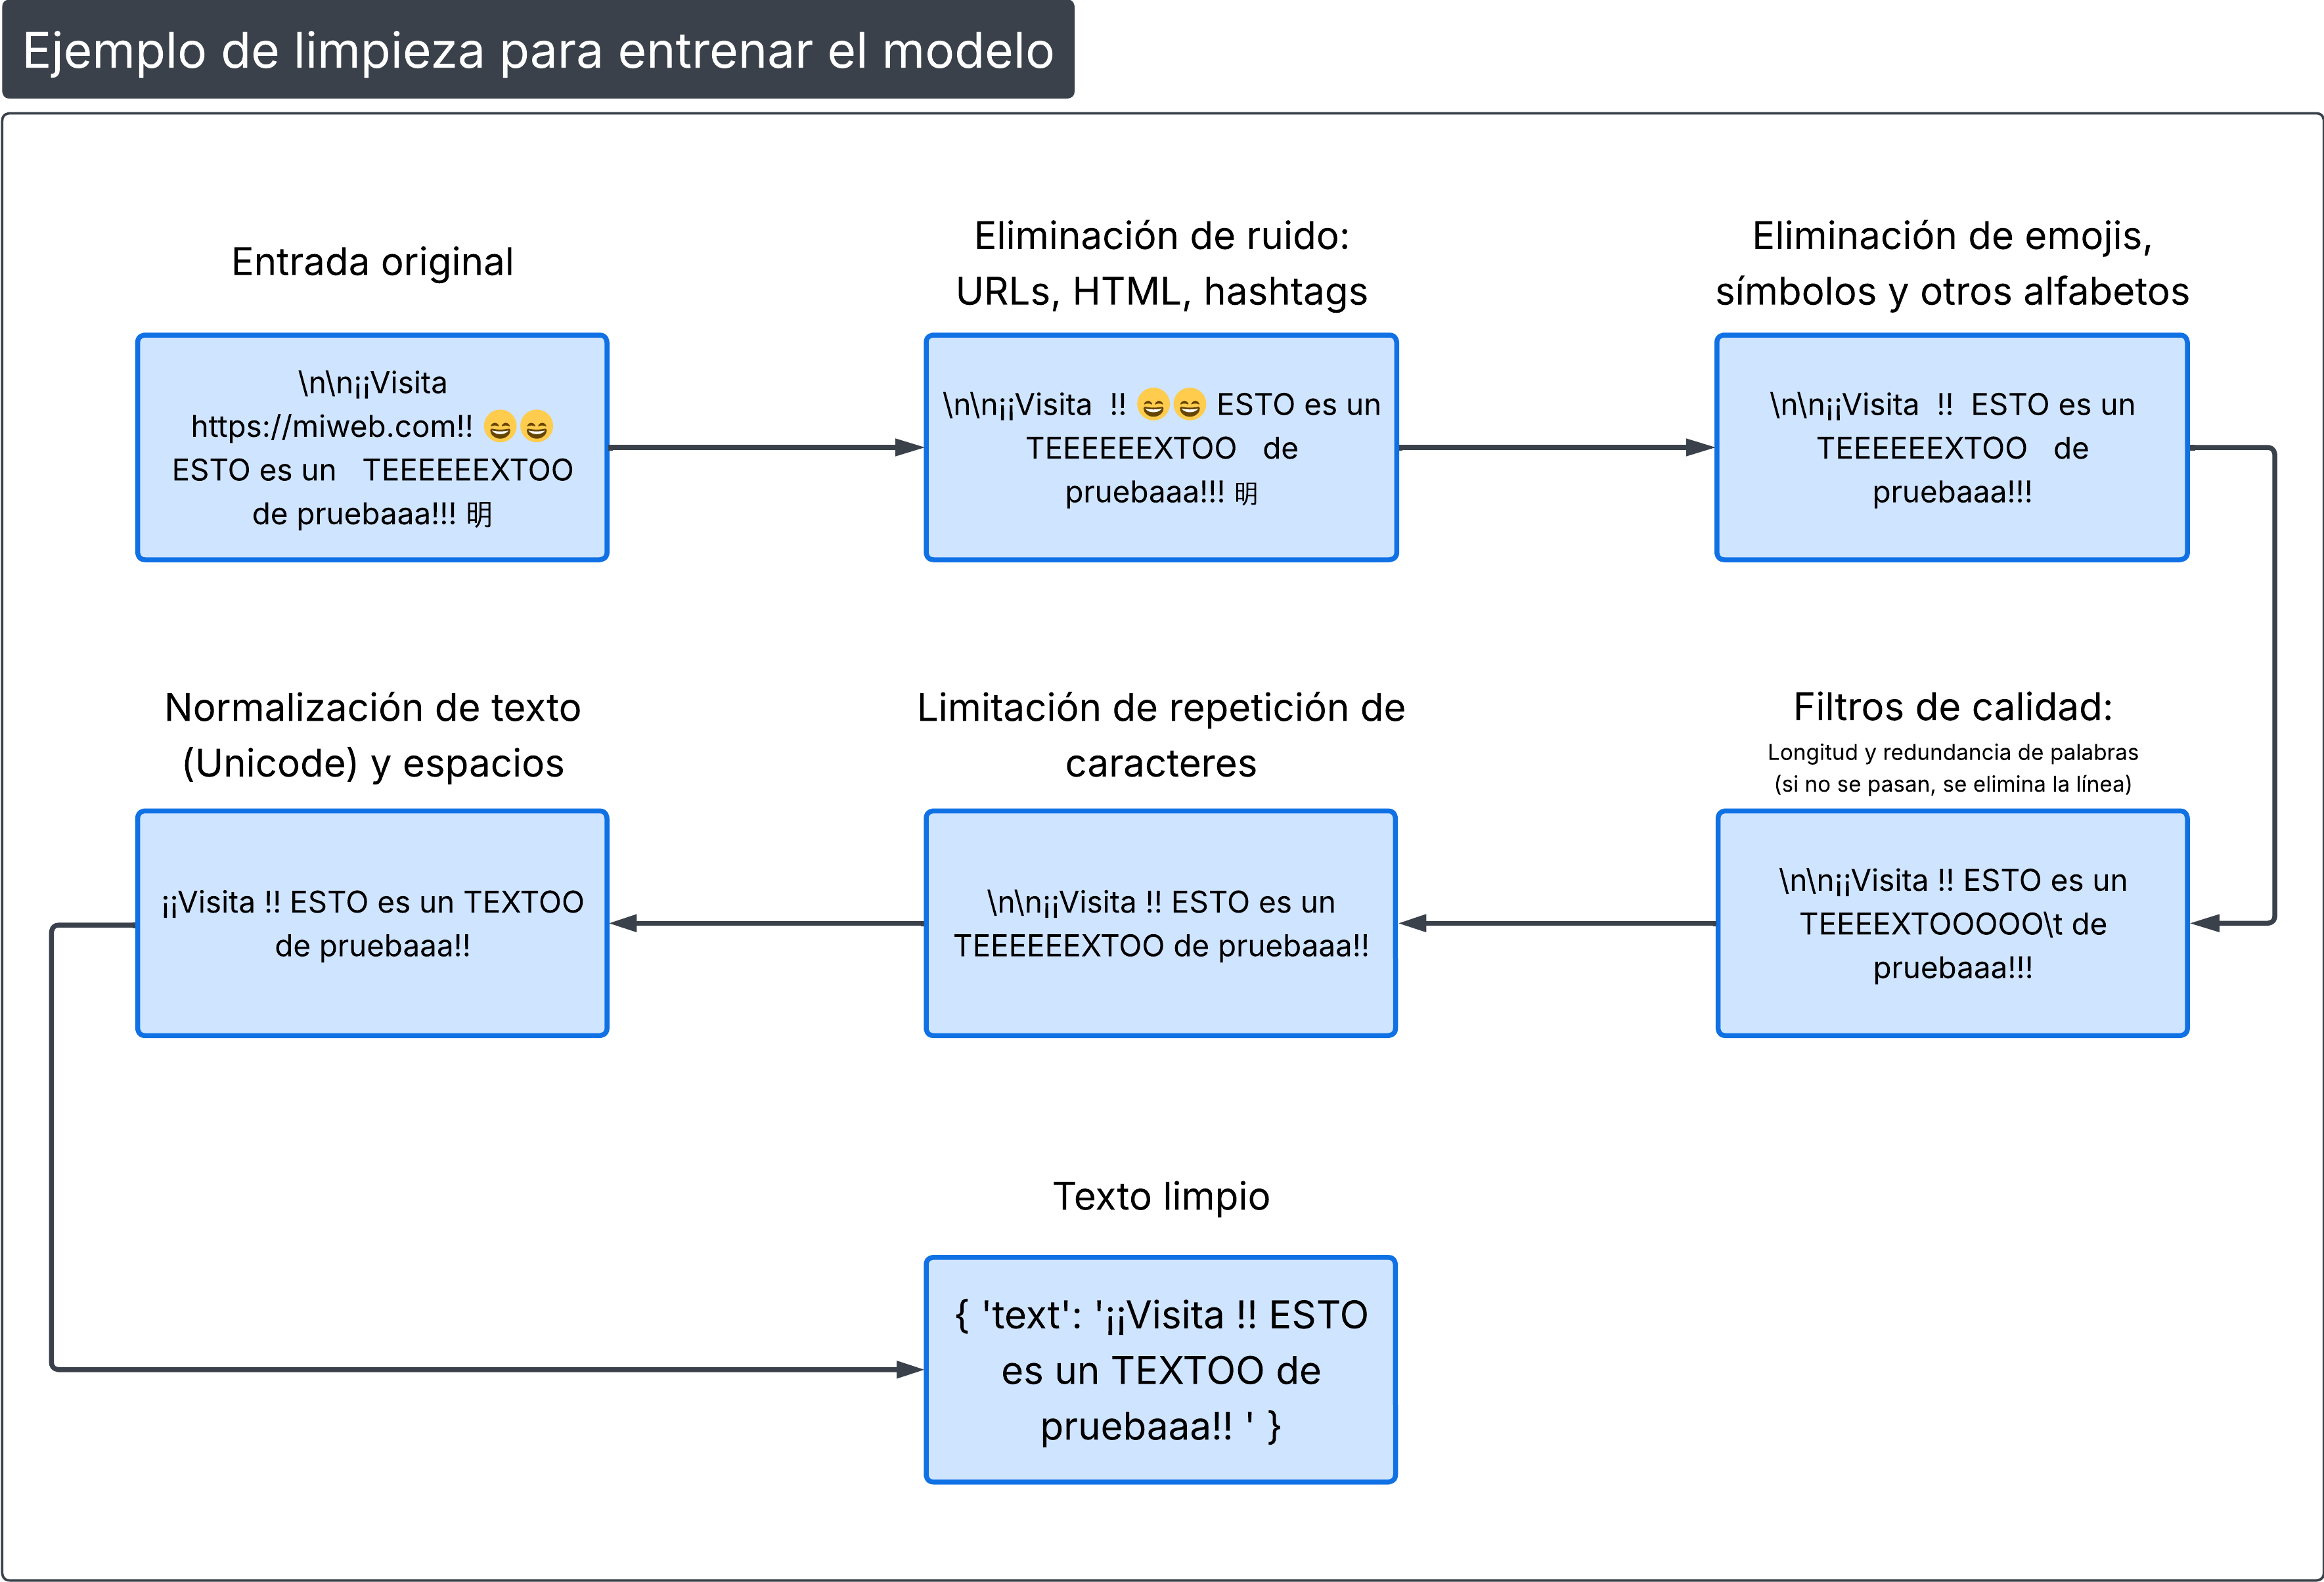
\includegraphics[width=1\textwidth]{figures/DiagramaLimpieza.png}    
    \caption{\label{fig:ejemplo-limpieza} Ejemplo de limpieza de una frase por el sistema. De creación propia.}
\end{figure}

Este proceso de limpieza permite obtener un corpus homogéneo, con una menor cantidad de ruido y adecuado para el análisis comparativo del rendimiento de los modelos de lenguaje seleccionados en lenguas minoritarias.

Aun así, después de analizar el dataset limpio, se observó que, pese a haberse limpiado correctamente, había algunas frases en otras lenguas como el inglés. Esto se debe a que los datasets obtienen mucha información de la web sin filtrarlo manualmente, capturando texto en multiples lenguas. Por eso, se aplicó después de la limpieza un filtro automático de detección de la lengua, con un umbral bajo, evitando borrar incorrectamente frases en la lengua objetivo por fallos en su detección automática, para intentar tener un corpus lo más homogeneo posible.

\subsection{Estadísticas de los datos}
\label{estadisticas-datos}

Tras el análisis de los \nameref{conjuntos-de-datos} disponibles para las tres lenguas objeto de estudio, se seleccionaron dos fuentes principales: el \textit{Corpus NOS} para el gallego y los datos de \textit{NLLB} (Opus) para el asturiano y el aranés. Estas colecciones proporcionan una cobertura amplia y heterogénea, aunque presentan diferencias significativas en longitud media, distribución de tokens y coherencia interna, lo que condicionó las decisiones de preprocesamiento descritas a continuación.

\subsubsection*{Procesamiento inicial y cálculo de estadísticas}

Para cada lengua se calcularon estadísticas de longitud, con el objetivo de caracterizar la distribución real de los datos y determinar valores adecuados de longitud de las muestras durante el entrenamiento. 

\paragraph{Asturiano (datos generales).}

El corpus de NLLB para el asturiano resultó ser el más problemático en términos de longitud. A pesar de contener más de medio millón de líneas, la mayoría eran extremadamente breves. La media fue de 48.14 tokens, la mediana de 42 y el percentil 95 de apenas 100 tokens. El máximo observado fue de 184 tokens y la moda aproximada se situó en torno a los 30 tokens.

\paragraph{Aranés (datos generales).}

El conjunto de datos de NLLB para el aranés contenía un número elevado de textos extremadamente breves. Aunque el corpus no era reducido en número de líneas, la presencia de tantos fragmentos cortos provocaba que el modelo tendiera a cerrar la generación de forma prematura durante las pruebas preliminares. Para intentar mitigar este problema, se aplicó un filtrado mínimo de 40 palabras por muestra, reteniendo únicamente ejemplos con suficiente contenido informativo. La distribución muestra una longitud media de 104.77 tokens, una mediana de 100 y un percentil 95 de 148 tokens. El máximo observado fue de 195 tokens y la moda aproximada se situó en torno a los 90 tokens.

\paragraph{Aranés (instructivo).}

El conjunto instructivo, compuesto por datos generados y pares pregunta–respuesta, presentó una distribución más dispersa y con colas largas. La media alcanzó los 287.15 tokens, con una mediana de 186 y un percentil 95 de 934 tokens. El máximo observado fue de 2\,013 tokens.

\paragraph{Gallego (datos generales).}

Para el gallego se empleó el \textit{Corpus NOS}, del cual se extrajeron fragmentos coherentes procedentes de Wikipedia, prensa, blogs, documentos oficiales y libros disponibles en el dataset. Tras el filtrado por idioma y la limpieza final, el corpus resultante mostró una media de 186.53 tokens, una mediana de 99 y un percentil 95 de 672 tokens. El máximo alcanzó los 5\,966 tokens, reflejando la presencia de textos sustancialmente más largos que en las otras lenguas.

\paragraph{Gallego (instructivo).}

El conjunto instructivo del gallego presentó una media de 311.26 tokens, una mediana de 208 y un percentil 95 cercano a los 983 tokens. El máximo observado fue de 1\,621 tokens.

\subsubsection*{Comparación entre lenguas y entre corpus raw e instructivo}

Las diferencias entre lenguas y entre tipos de corpus son sustanciales y tienen implicaciones directas en el diseño del entrenamiento. Los corpus generales de asturiano y aranés presentan longitudes significativamente menores que el corpus NOS en gallego. 

Los corpus instructivos muestran patrones similares entre lenguas: distribuciones más amplias, colas largas y mayor variabilidad. La media oscila entre 210 y 311 tokens, muy por encima de los corpus generales. Esta diferencia confirma que los instructivos aportan ejemplos más largos y estructurados, esenciales para mejorar la capacidad del modelo para responder preguntas y mantener coherencia en textos extensos.

\subsubsection*{Comparativa de estadísticas entre lenguas}

\begin{longtable}{@{}llrrrrrrr@{}}
\caption{Resumen comparativo de estadísticas de longitud para los corpus generales e instructivos de las tres lenguas.}
\label{tab:estadisticas_globales} \\
\toprule
Lengua & Tipo & Media & Mediana & P95 & P98 & Máx. & Mín. & Moda \\ 
\midrule
\endfirsthead

\multicolumn{9}{c}{\tablename\ \thetable{} -- continuación} \\
\toprule
Lengua & Tipo & Media & Mediana & P95 & P98 & Máx. & Mín. & Moda \\ 
\midrule
\endhead

\midrule \multicolumn{9}{r}{Continúa en la siguiente página} \\
\endfoot

\bottomrule
\endlastfoot

Asturiano & General & 48.14 & 42 & 100 & 120 & 184 & 6 & 30 \\
Asturiano & Instructivo & 210.13 & 112 & 740.9 & 910.8 & 1453 & 20 & 40 \\

Aranés & General & 104.77 & 100 & 148 & 159 & 195 & 57 & 90 \\
Aranés & Instructivo & 287.15 & 186 & 934 & 1101 & 2013 & 26 & 50 \\

Gallego & General & 186.53 & 99 & 672 & 1087.08 & 5966 & 28 & 70 \\
Gallego & Instructivo & 311.26 & 208 & 982.7 & 1151.8 & 1621 & 19 & 30 \\

\end{longtable}

\begin{figure}[H]
    \centering
    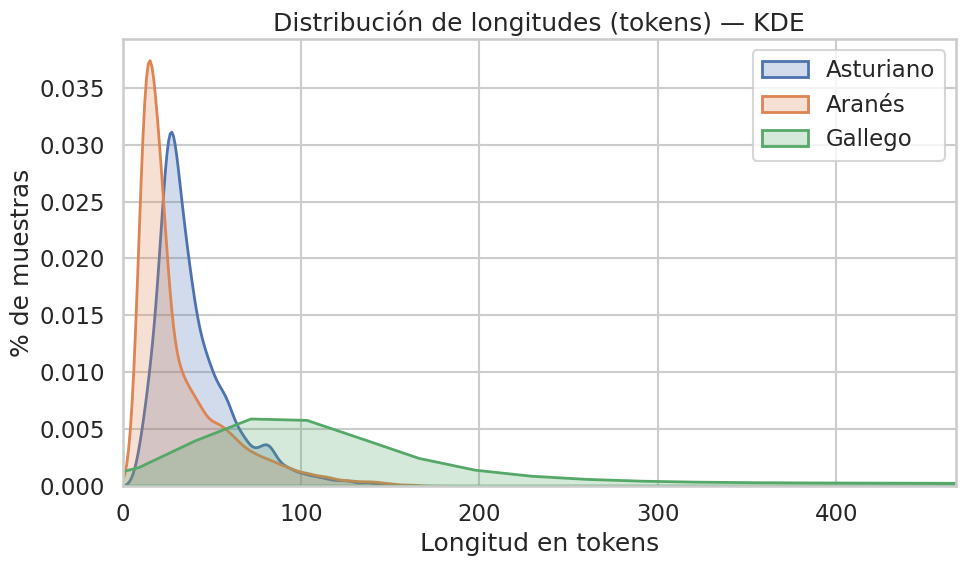
\includegraphics[width=0.8\textwidth]{figures/KDE_DistribucionLongitudTokensARNOriginal.png}    
    \caption{\label{fig:distribucion-longitudes-arn-original}Distribución de longitud de las muestras por lengua en los datasets originales. De creación propia.}
\end{figure}

Como se puede ver en la Figura \ref{fig:distribucion-longitudes-arn-original}, el Aranés tiene la mayoría de muestras demasiado pequeñas y se ha visto que afecta al entrenamiento. Por lo que se ha filtrado a 40 el mínimo de palabras en las muestras del dataset de entrenamiento del aranés, cambiando su distribución como se puede observar en la siguiente Figura \ref{fig:distribucion-longitudes}. También se puede ver como el dataset del gallego es de mucha mejor calidad, con unas muestras con longitudes mucho más distribuidas. Ambas estadísticas son con los datasets ya limpios y filtrados.

\begin{figure}[H]
    \centering
    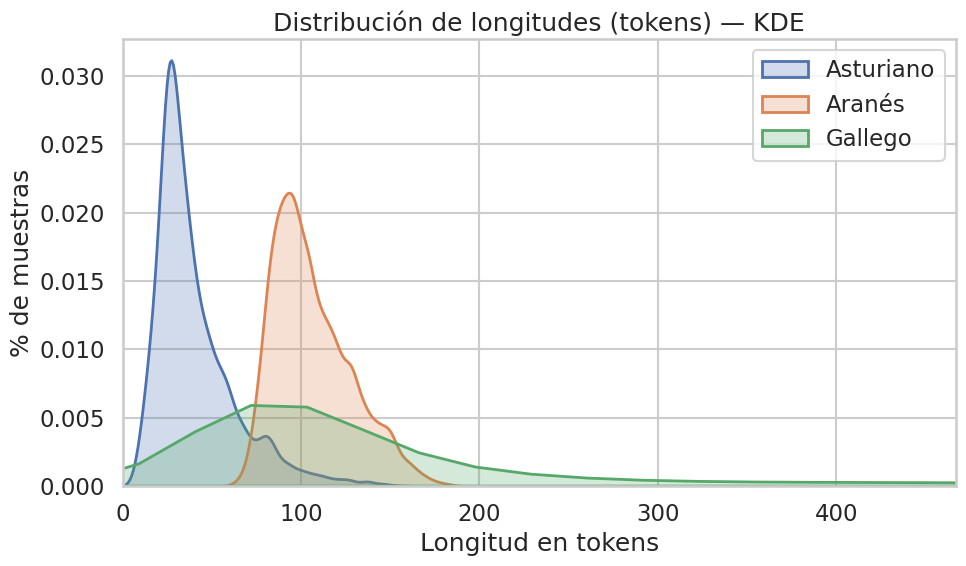
\includegraphics[width=0.8\textwidth]{figures/KDE_DistribucionLongitudTokens.png}    
    \caption{\label{fig:distribucion-longitudes}Distribución de longitud de las muestras por lengua en los datos de entrenamiento. De creación propia.}
\end{figure}



\subsection{Implicaciones para el entrenamiento}

Las diferencias entre lenguas y tipos de corpus condicionaron directamente el diseño del conjunto de entrenamiento. En el caso del asturiano y el aranés, la abundancia de textos breves obligó a aplicar filtrados mínimos y a seleccionar cuidadosamente el valor de \texttt{max\_length}, mientras que en el gallego fue necesario controlar la presencia de textos extremadamente largos para evitar desbordamientos de memoria durante el entrenamiento.

El uso de datos instructivos permitió complementar los corpus generales con ejemplos más largos y estructurados, mejorando la capacidad del modelo para responder preguntas y mantener coherencia en textos extensos. Esta estrategia resultó especialmente útil en lenguas con corpus generales muy breves, como el asturiano.

\subsection{Datos instructivos y generación sintética}
\label{datos-instructivos}

El entrenamiento de un modelo en modo \textit{Causal LM} (Modelado de Lenguaje Causal) permite que este aprenda la distribución de probabilidad de los nuevos tokens respecto a su contexto. Sin embargo, esta aproximación por sí sola no garantiza que el modelo adquiera la capacidad de interactuar de forma directa con un usuario, responder preguntas de manera coherente o asimilar un formato puramente instructivo. 

Para mitigar esta limitación y guiar al modelo hacia un comportamiento de asistente, se diseñó un flujo de trabajo para la obtención de un conjunto de datos instructivos sintéticos. Como modelo generador principal se empleó el modelo de gran tamaño \textit{GPT-OSS 120B} a través de la API de Groq, tomando como base oraciones breves extraídas del corpus de \textit{Tatoeba} para las tres lenguas de bajos recursos objeto de estudio: asturiano, gallego y aranés. 

Con el propósito de dotar de una mayor diversidad al corpus y exponer al modelo a secuencias de texto más largas dentro de las restricciones impuestas por la VRAM disponible, la generación automatizada se dividió en dos estrategias diferenciadas mediante ingeniería de instrucciones (\textit{prompt engineering}):

\begin{itemize}
    \item \textbf{Transformación y ampliación de textos:} Esta estrategia entrena al modelo en tareas de reescritura y expansión lingüística. Se utilizaron plantillas que exigían al modelo generador realizar diferentes tareas a partir de una oración de Tatoeba: desarrollar el contenido añadiendo detalles, dar consejos, cambiar el registro a formal o informal, o parafrasear la información. 
    
    Para facilitar el procesamiento de las respuestas del modelo a nivel de código, se forzó al generador a encapsular su salida bajo etiquetas XML (\texttt{<respuesta>...</respuesta>}), facilitando su posterior estructuración en el formato de turnos conversacionales utilizado en el ajuste fino.
    
    A continuación, se ilustra el resultado de este proceso con un ejemplo real extraído del corpus generado para el asturiano:
    
    \begin{quotation}
        \noindent\textbf{Texto base (Tatoeba):} \textit{Tas buenu pa dir a nengún sitiu.}\\
        \textbf{Instrucción aplicada:} \textit{Da un conseyu relacionáu con esti conteníu:}\\
        
        \noindent\textbf{Formato estructurado final:}
       \begin{verbatim}
<​|user|>
Da un conseyu relacionáu con esti conteníu:
Tas buenu pa dir a nengún sitiu.
<​|assistant|>
Si sientes que tas buenu pa dir a nengún sitiu, ye importante 
reflexonar sobre a quién quies dir la mensaxe y por qué. Escueyi 
un destinatariu concretu, adapta'l tonu al so públicu y sé claru 
col conteníu. Así, la comunicación será más eficaz y evites 
perder oportunidaes por hablar en llugar que nun tien audiencia.
\end{verbatim}
    \end{quotation}

    \item \textbf{Comprensión lectora (Pregunta - Respuesta):} Orientada a dotar al modelo de la capacidad de extracción de información y síntesis precisa. Mediante plantillas específicas (\textit{QA Templates}), se suministró un texto base al modelo generador con la instrucción de formular una pregunta lógica y directa sobre el mismo, acompañada de su respectiva respuesta detallada. El formato de salida de la API se restringió estrictamente mediante bloques diferenciados (\texttt{<pregunta>} y \texttt{<respuesta>}).
    
    Un ejemplo representativo del resultado de esta estrategia, también sobre el corpus en asturiano, se detalla a continuación:

    \begin{quotation}
        \noindent\textbf{Texto base (Tatoeba):} \textit{El cielu del atapecer ye roxu.}\\
        \textbf{Instrucción aplicada:} \textit{Inventa una pregunta sencilla sobre esti fragmentu y da una respuesta curtia pero natural.}\\
        
        \noindent\textbf{Formato estructurado final:}
        \begin{verbatim}
<|user|>
¿Por qué'l cielu del atapecer ye roxu?
<|assistant|>
Porque la dispersión de la lluz del Sol pola atmósfera fai que la 
lluz azul se disperse y solo quede la lluz roja visible.
        \end{verbatim}
    \end{quotation}
\end{itemize}

Los conjuntos de datos que se han generado y utilizado para el entrenamiento se encuentran disponibles en HuggingFace con el resto de materiales del TFG \url{https://hf.co/collections/MiguelGP-13/tfg} \cite{lexicons_2025, galician_instructive_2025, asturian_instructive_2025, aranes_instructive_2025, asturian_annotated_2025, galician_annotated_2025, aranes_annotated_2025, asturian_cloze_2025, galician_cloze_2025, aranes_cloze_2025}.

\subsubsection{Robustez del flujo y control de calidad}
Debido a que las respuestas de los modelos de lenguaje pueden sufrir alucinaciones de formato o errores de truncado en la API, el script implementado en Python incorporó filtros heurísticos automatizados de validación. Tras cada llamada al modelo, el sistema verifica la presencia íntegra de las etiquetas delimitadoras requeridas y comprueba que la longitud de los textos generados cumpliera con unos umbrales mínimos de calidad. 

Dado que el objetivo metodológico consistía en equilibrar estrictamente el volumen de datos por lengua y tarea, se adoptó un enfoque de ejecución por cuotas. El algoritmo descartaba de manera transparente cualquier salida defectuosa o mal formateada y continuaba realizando peticiones de forma iterativa hasta asegurar un total exacto de $N=500$ ejemplos instructivos válidos y limpios para cada uno de los subconjuntos, garantizando así la homogeneidad del corpus final de entrenamiento.


\section{Preparación del modelo}

Tras la evaluación de distintos modelos base, se seleccionó \textbf{Qwen-2.5 7B} cuantizado a 4 bits como punto de partida para este trabajo. Esta elección se debe a que ofrece un equilibrio adecuado entre capacidad de comprensión, calidad generativa y conocimiento de las lenguas de estudio, como puede verse en los \nameref{ch:Resultados base}.

\subsection{Capas del Lora}

Se ha decidido aplicar los adaptadores LoRA  específicamente sobre las capas de atención (\texttt{q\_proj}, \texttt{k\_proj}, \texttt{v\_proj}), la capa Output Projection (\texttt{o\_proj}), encargada de combinar la información de todas las cabezas de atención y proyectarla de vuelta al tamaño original del modelo, y las capas de la etapa de feed forward (\texttt{gate\_proj}, \texttt{up\_proj} y  \texttt{down\_proj}) del Transformer.
La selección de estas capas responde a criterios tanto teóricos como empíricos. Por un lado, las proyecciones de atención constituyen el núcleo del mecanismo de atención, responsable de modelar las relaciones contextuales entre los elementos de una secuencia. Modificar estas matrices permite ajustar de manera directa cómo el modelo interpreta y pondera la información lingüística.

Por otro lado, las capas del MLP son las encargadas de transformar las representaciones internas y aportar capacidad expresiva adicional. Estudios previos sobre adaptadores, como AdapterFusion \cite{pfeiffer2021adapterfusionnondestructivetaskcomposition}, muestran que insertar módulos entrenables en estas capas permite modificar el comportamiento del modelo sin alterar los pesos originales, manteniendo así la integridad del modelo base y evitando efectos destructivos.

\subsection{Configuración inicial de hiperparámetros}

La configuración de hiperparámetros es un componente esencial en el proceso de entrenamiento, especialmente en contextos con recursos computacionales limitados y cuando se emplean técnicas como QLoRA. El Cuadro \ref{tab:hiperparametros_iniciales} resume los parámetros principales y los valores seleccionados.

\begin{table}[H]
\centering
\begin{tabular}{l l}
\hline
\textbf{Hiperparámetro} & \textbf{Valor} \\
\hline
Rango LoRA (\texttt{r}) & 8 \\
Alpha & 16 \\
Dropout & 0.1 \\
Batch size & 2 \\
Épocas de entrenamiento & 2 \\
Learning rate & 1e-4 \\
Scheduler & Cosine \\
Warmup ratio & 0.1 \\
Optimizador & Paged AdamW 32-bit \\
\hline
\end{tabular}
\caption{Hiperparámetros iniciales.}
\label{tab:hiperparametros_iniciales}
\end{table}

\subsubsection{Parámetros de LoRA}

\paragraph{Rango (\texttt{r} = 8).}
El rango determina la dimensionalidad interna de los adaptadores LoRA. Un valor de 8 proporciona un equilibrio adecuado entre capacidad de adaptación y eficiencia computacional. Valores mayores permiten aprender representaciones más complejas, pero incrementan el número de parámetros entrenables y el riesgo de sobreajuste, especialmente en escenarios de bajo recurso como este.

\paragraph{Alpha = 16.}
Este parámetro actúa como un factor de escalado que controla la contribución de los adaptadores respecto al modelo base. Un valor moderado como 16 permite una adaptación estable sin introducir oscilaciones excesivas en el gradiente.

\paragraph{Dropout = 0.1.}
Se introduce un pequeño dropout para reducir el sobreajuste. Dado que el corpus es relativamente reducido y homogéneo, este valor ayuda a mejorar la generalización sin afectar negativamente a la estabilidad del entrenamiento.

\subsubsection{Parámetros de entrenamiento}

\paragraph{Batch size = 1 y Gradient Accumulation = 2.}
Las limitaciones de memoria de la GPU impiden utilizar batch sizes mayores. Para compensarlo, se acumulan gradientes durante dos pasos, obteniendo un batch efectivo de tamaño 2. Esto mejora la estabilidad del entrenamiento sin incrementar el uso de memoria.

\paragraph{Learning rate = 1e-4.}
Los modelos adaptados mediante LoRA toleran tasas de aprendizaje más altas que los modelos entrenados desde cero. 

\paragraph{Épocas = 2.}
El número de épocas se mantiene bajo debido al coste computacional del entrenamiento y al riesgo de sobreajuste en un corpus pequeño.

\subsubsection{Scheduler, warmup y optimizador}

\paragraph{Scheduler cosenoidal.}
El scheduler cosenoidal reduce progresivamente la tasa de aprendizaje, favoreciendo una convergencia más suave y estable. Este tipo de scheduler es especialmente útil en entrenamientos cortos, donde los cambios bruscos pueden afectar negativamente al rendimiento.

\paragraph{Warmup ratio = 0.1.}
Durante el 10\% inicial del entrenamiento, la tasa de aprendizaje aumenta gradualmente. Esto evita picos de gradiente al inicio, que son especialmente problemáticos en modelos cuantizados y con adaptadores LoRA.

\paragraph{Paged AdamW 32-bit.}
Este optimizador está diseñado específicamente para QLoRA, gestionando eficientemente los pesos cuantizados y reduciendo el uso de memoria mediante paginación.


\section{Entrenamiento del modelo}

Para definir la mejor manera de entrenar, se han realizado pruebas iniciales con el asturiano, y luego se han probado la mejor metodología encontrada en el aranés y el gallego, adaptándose a los corpus de cada lengua y analizando los resultados.

Los modelos entrenados en todas las lenguas y con todas las configuraciones se encuentran disponibles en HuggingFace con el resto de materiales del TFG \url{https://hf.co/collections/MiguelGP-13/tfg} \cite{asturian_lora_2025, asturian_concat_2025, asturian_concat_instructive_2025, galician_lora_2025, aranes_lora_2025, aranes_lora_instructive_2025}.

\subsection{Optimización de la longitud de las muestras}
\label{problemas-longitud-muestra}

Los primeros experimentos de entrenamiento se realizaron utilizando una versión tokenizada del corpus con una longitud fija de 512 tokens por muestra. Esta decisión inicial, aunque habitual en muchos flujos de trabajo, resultó poco adecuada para nuestros datos, ya que tras analizar el conjunto de datos, se observó que la longitud media de las frases era cercana a los 50 tokens, lo que implicaba que la mayor parte de cada entrada estaba compuesta por \textit{padding}. Como consecuencia, el modelo aprendió que el token más frecuente era el token de fin de secuencia, produciendo respuestas vacías o extremadamente breves. 

Para solucionar esto, en vez de poner una longitud definida de los datos, se investigó emplear el percentil 95 o 98 de la cantidad de tokens por frase como referencia para determinar la longitud máxima razonable, evitando tanto el truncado excesivo como la inclusión de demasiado padding. Además se vió que por limitaciones de cómputo, el máximo absoluto por muestra es de 160 tokens, ya que si las secuencias son más largas, el servidor devolvía OoME (Out of Memory Error), es decir, que la tarjeta gráfica no tiene más espacio en la memoria VRAM.


Una vez ajustada la longitud máxima a valores más acordes con la distribución real del corpus, el modelo comenzó a generar texto de forma más consistente. Aun así, continuaba produciendo \textbf{respuestas cortas o incompletas}. Como aspecto positivo, al evaluar estos primeros modelos se observó que, pese a su baja fluidez, mostraban una mejora apreciable en tareas de corrección ortográfica y morfológica. Esto sugiere que el modelo sí estaba captando patrones lingüísticos relevantes, aunque todavía no era capaz de producir textos extensos o naturales.

La única solución real para mitigar este problema es tener muestras más largas. Para ello, se probó a \textbf{concatenar varias frases del dataset en una}, aumentando la longitud efectiva de las muestras y proporcionando al modelo contextos más ricos y coherentes. Sin embargo, esta aproximación tiene dos problemas. El primero y menos importante para este estudio, es que reduce el número de muestras diponibles aun más en un dataset ya bastante reducido. Debido a la capacidad de cómputo disponble, no se va a poder entrenar sobre el dataset entero, por lo que este problema no afectaría al proyecto. El segundo problema y más importante, es que al concatenar frases que no tienen por que tener nada que ver entre sí, se ha visto que hace que el modelo pierda conocimiento de como generar texto de manera coherente, mezclando frases una detrás de otra sin tener siempre conexión entre ellas. Para conseguir textos más largos, coherentes y de mayor variedad temática, se contactó con la \textbf{Academia de la Llingua Asturiana} \cite{ALLA2024}, para solicitar el uso de los artículos y publicaciones de sus revistas digitales. Hasta el momento de entrega de este TFG no se ha recibido respuesta.

 Después de aplicar el cambio de concatenar muestras del conjunto de datos y corrección de la longitud de las muestras, el modelo empezó a generar textos más largos en asturiano, pero perdió bastante coherencia, por lo que empezó a responder las preguntas peor. 
 
 Para intentar evitarlo, se ha decidido probar a hacer un entrenamiento final con \nameref{datos-instructivos} con prompt y respuesta coherentes al modelo concatenado generados automáticamente.
 
\subsection{Optimización de hiperparámetros}
 No se han observado grandes variaciones al optimizar los hiperparámetros. Se optó por reducir la tasa de aprendizaje (\textit{learning rate}) e incrementar la acumulación de gradientes (\textit{gradient accumulation}). El objetivo de esta configuración es mitigar el sobreajuste (\textit{overfitting}) del conjunto de datos y evitar actualizaciones de pesos excesivamente abruptas que puedan derivar en el fenómeno de olvido catastrófico \cite{luo2023an}. 
 
\subsection{Análisis cualitativo de las pruebas en asturiano}
Los ejemplos cualitativos tanto del asturiano como de las otras lenguas se encuentran en los \nameref{resultados_cualitativos_qlora}.
En los ejemplos cualitativos se puede ver como el concatenado escribe respuestas mucho más extensas y ricas, pero cambiando completamente de tema repentinamente, mientras que el modelo entrenado con frases más cortas es más conciso, a veces demasiado.

En estos y otros ejemplos, se observó que el modelo generaba con bastante frecuencia sobre temas muy específicos, como aspectos políticos, legales o historia. Esto probablemente se debe a la alta prevalencia en el dataset de estos temas y se estudiará como se comportan los modelos en las otras lenguas.

 \subsection{Metodología para aranés y gallego}
 Con los resultados obtenidos de las pruebas del asturiano, se va a entrenar los modelos en las otras lenguas. 
 Se ha visto que concatenar no aporta valor, por lo que se entrenará con los textos más largos encontrados en el dataset, pero sin concatenar muestras. Se cortarán los datos al percentil 95 del dataset y posteriormente, cuando el modelo haya aprendido la lengua, si el modelo ha perdido cohesión en la generación, se entrenará con los datasets sintéticos instructivos para obligar al modelo a seguir mejor el estilo y no acabar las respuestas demasiado pronto.

 \subsubsection{Aranés}
 El conjunto de datos del Aranés tiene muchas muestras muy cortas, con una mediana de 22 tokens y una moda de 10 tokens. Por lo que al entrenar, tenía el mismo problema que el asturiano, generando texto muy corto. El problema es que si le fuerzas a sacar un mínimo de tokens, en vez de generar texto como el modelo de asturiano, generaba puntos, queriendo acabar las frases desde el principio. Por lo que como diferencia con los otros dos modelos, se filtró su dataset cogiendo las muestras con mínimo 40 palabras. Esto redujo mucho el tamaño del dataset y enseña al modelo a generar siempre contenido largo, lo cual tampoco es perfecto, pero si mejor que que no genere nada. En los resultados de la sección \ref{tab:metricas_calidad_lengua_Aranés} se puede ver que consigue que el modelo genere texto, pero de peor calidad.

 \subsubsection{Gallego}
El gallego, como lengua oficial de Galicia, pese a ser una lengua minoritaria, tiene una cantidad de datos disponibles mucho mayor, haciendo posible un entrenamiento mejor con una longitud media de las muestras y una variedad temática mayor. Por esta disponibilidad de datos de mayor calidad, el modelo solo se ha entrenado con muestras seleccionadas, sin concatenar ni necesitar los datos instructivos generados.
Los datos al contrario que en las otras dos lenguas, venían en documentos largos en vez de directamente en frases. Esto permite coger muestras coherentes y cohesionadas sin importar la longitud, dando un entrenamiento mucho mejor.

\subsection{Longitud de entrenamiento y dinámica de la función de pérdida}
\label{subsec:longitud_entrenamiento}

En la Figura \ref{fig:comparativa-loss} se analiza la evolución de la función de pérdida (\textit{loss}) a lo largo de los pasos de entrenamiento para los distintos modelos. En el contexto del \textit{fine-tuning} mediante QLoRA usando Casual LLM, el \textit{loss} utilizado es la entropía cruzada (\textit{cross-entropy loss}) \cite{vaswani2023attentionneed}. Esta métrica cuantifica la discrepancia entre la distribución de probabilidad predicha por el modelo para el siguiente \textit{token} y el \textit{token} real (\textit{ground truth}) del texto de entrenamiento. Por tanto, su medición y evolución temporal son indicadores críticos de la convergencia del modelo: un descenso sostenido demuestra que la red está optimizando sus adaptadores de bajo rango para capturar los patrones lingüísticos y semánticos del nuevo corpus.

\begin{figure}[H]
    \centering
    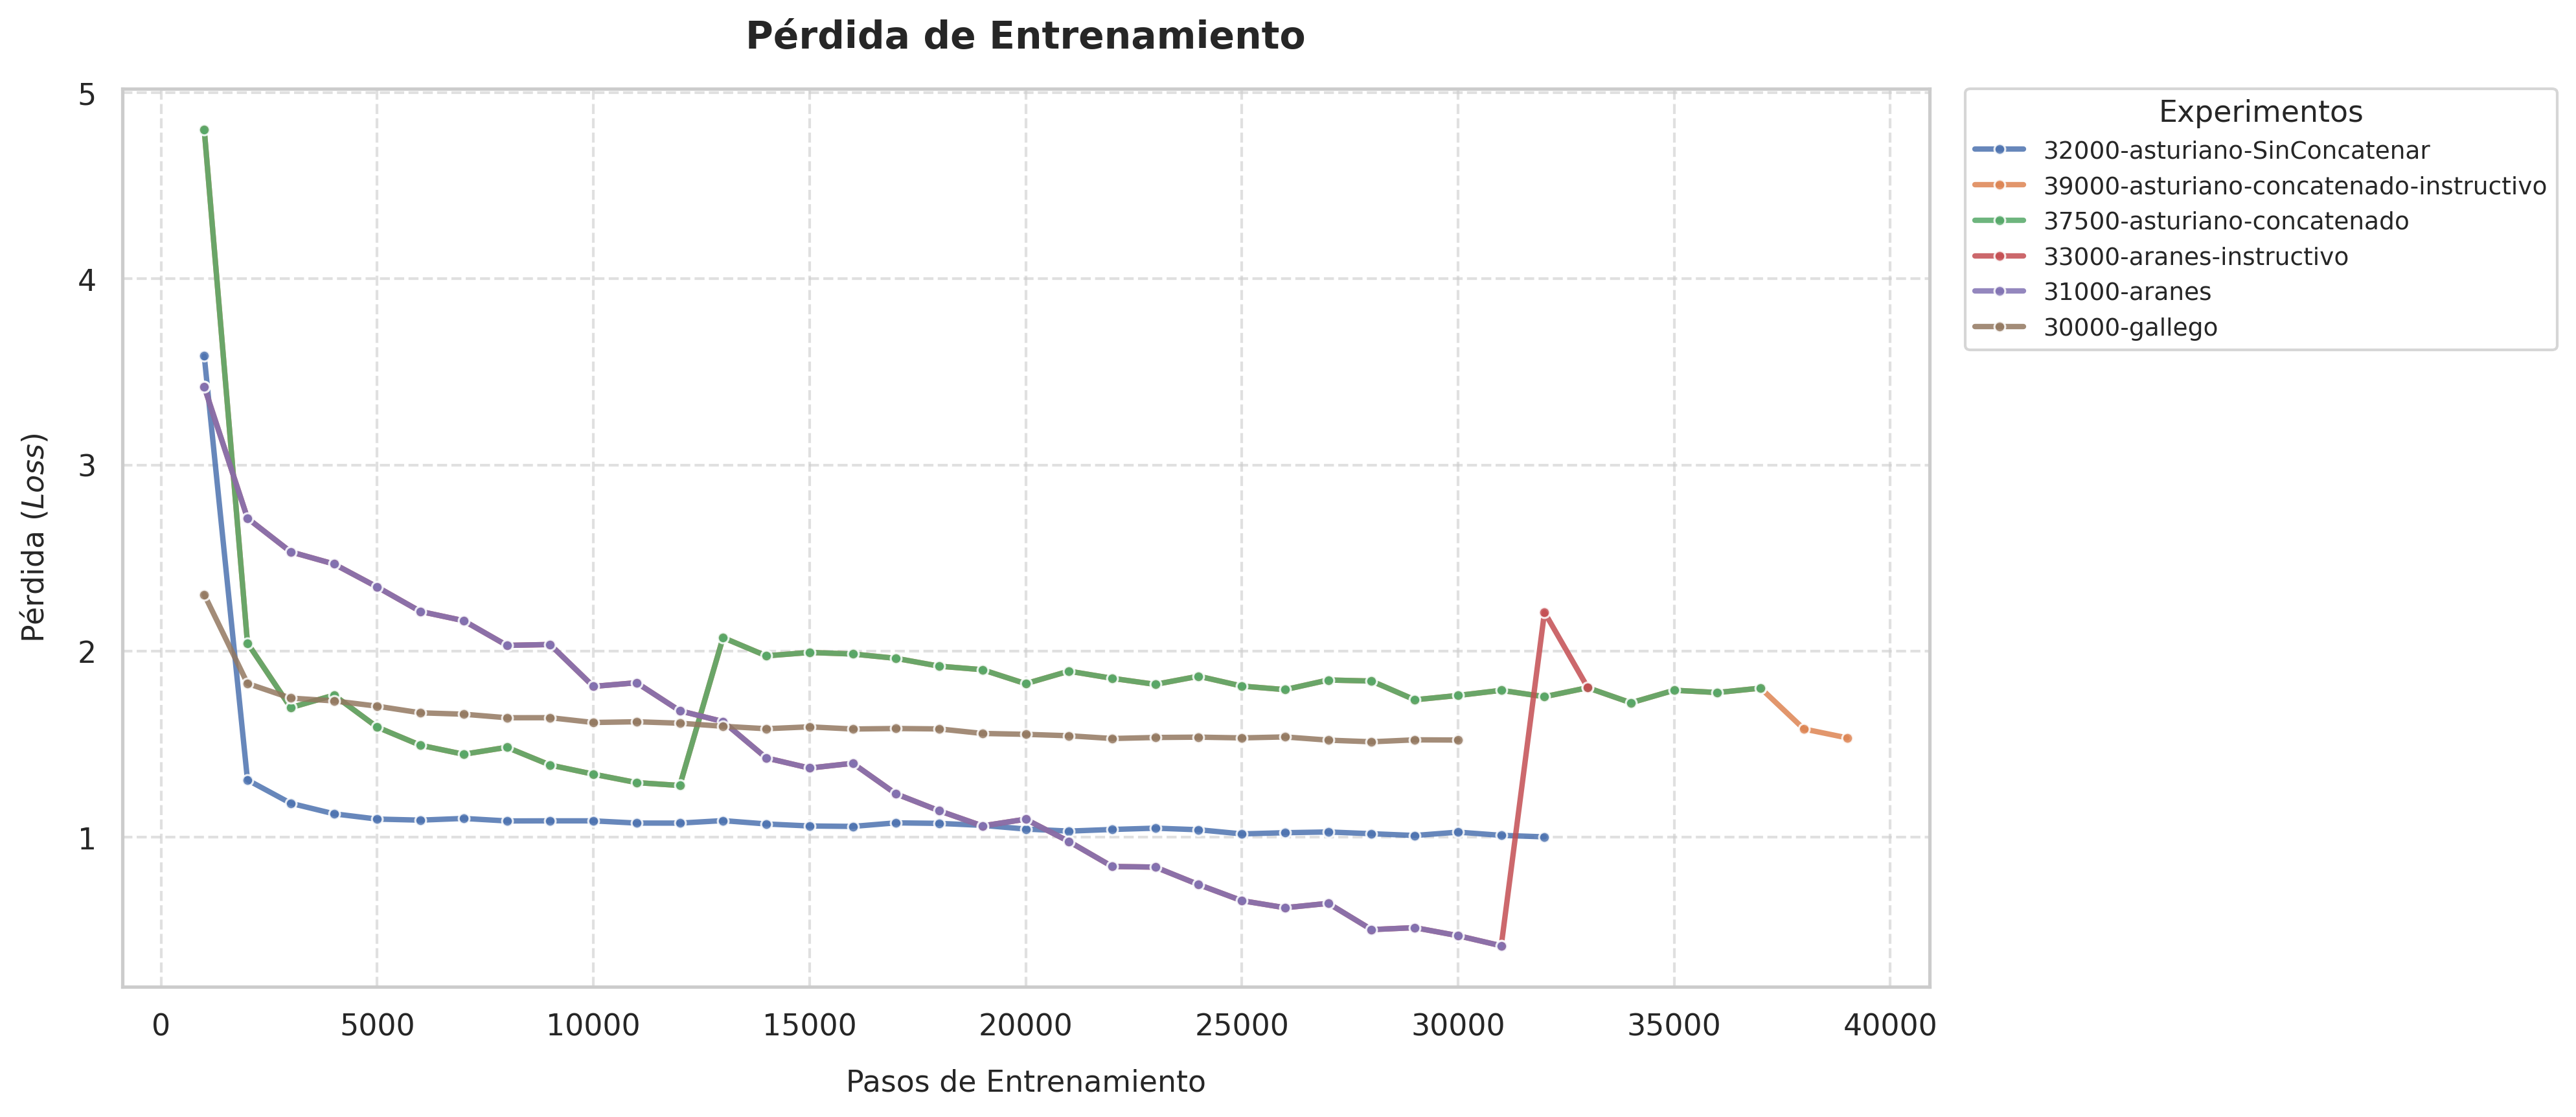
\includegraphics[width=1\textwidth]{figures/comparativa_loss.png}    
    \caption{Comparativa de funciones de pérdida de entrenamiento. De creación propia.}
    \label{fig:comparativa-loss}
\end{figure}

A partir de las curvas obtenidas, se observa que los entrenamientos del modelo para el gallego y el asturiano sin concatenar presentan las dinámicas más estables. El modelo de gallego estabiliza su pérdida en un valor ligeramente más alto, un comportamiento esperado debido a la alta variedad y riqueza del conjunto de datos utilizado, lo que dificulta que la entropía cruzada llegue a valores cercanos a cero pero garantiza una mayor capacidad de generalización.

Por su parte, el modelo del aranés es el que presenta el descenso de pérdida más rápido. Al tratarse del conjunto de datos más reducido, esta abrupta caída sugiere que el modelo sufría un leve sobreajuste (\textit{overfitting}), memorizando las secuencias en lugar de aprender sus estructuras subyacentes. Esto explica por qué, al cambiar los datos al modo instructivo en fases posteriores, el \textit{loss} inicial se eleva de manera tan notable ante la introducción de formatos no vistos.

Por último, el modelo asturiano concatenado muestra la curva más inestable y alta, lo cual se atribuye a que las muestras concatenadas de forma contigua introducen rupturas de contexto que resultan caóticas para el modelado de lenguaje causal. Sin embargo, se constata que la posterior introducción de las muestras instructivas, significativamente más estructuradas y delimitadas, corrige esta tendencia inestable, permitiendo una optimización más eficiente y mejorando el rendimiento general del entrenamiento.
\chapter{Fase 3: Evaluación del modelo y comparativa}
\label{ch:benchmark}

Los métodos habituales para evaluar modelos de lenguaje se basan en conjuntos de datos creados manualmente, que incluyen tareas de preguntas y respuestas, razonamiento o comprensión lectora \cite{perez-ortiz-etal-2024-expanding, gonzalez2026iberbench, srivastava2022bigbench}. Sin embargo, en el ámbito de las lenguas minoritarias estos recursos no existen o son extremadamente limitados, y su creación requiere un esfuerzo de anotación que no siempre es viable. Esta falta de datos dificulta la evaluación sistemática de modelos adaptados a lenguas de bajo recurso y limita la comparación entre enfoques.

Ante esta situación, se propone un benchmark diseñado para depender del mínimo número posible de datos en la lengua objetivo. El enfoque se basa en tareas lingüísticas fundamentales: generación de texto libre, traducción, inferencia de palabras enmascaradas y corrección de errores gramaticales, que pueden evaluarse a partir de texto monolingüe y, cuando está disponible, de un pequeño conjunto de datos paralelos. De este modo, es posible estimar la capacidad del modelo para generar texto correcto y coherente en la lengua objetivo sin necesidad de construir manualmente conjuntos de evaluación complejos.

El benchmark está concebido para ser reutilizable en otras lenguas minoritarias, siempre que exista un corpus básico en la lengua objetivo y, opcionalmente, un conjunto reducido de pares de traducción. Aunque este enfoque no evalúa conocimiento cultural o razonamiento profundo, sí permite medir de forma fiable la competencia lingüística del modelo, proporcionando una herramienta práctica y reproducible para el estudio de lenguas con recursos limitados.

\section{Métricas para la evaluación del modelo propuesto}

Como se ha introducido, ante la ausencia de datasets supervisados de evaluación para el asturiano o el aranés, se propone un conjunto de métricas cuantitativas centradas en la comprensión, generación y adecuación del modelo en la nueva lengua. Al adaptar un modelo que ya ha adquirido conocimiento general previo en su etapa de preentrenamiento, se asume que su rendimiento en tareas lógicas o de razonamiento se mantendrá estable, por lo que el foco de este benchmark se desplaza hacia la evaluación de su competencia y madurez puramente lingüística.

\subsection{Estudio de calidad de lengua}
\label{calidad-lengua}

El benchmark está diseñado para medir la competencia lingüística del modelo en la lengua objetivo, evaluando en primer lugar su capacidad para generar texto fluido, morfológicamente correcto y estructuralmente natural. Esta primera sección aborda de manera directa dos de las principales dimensiones de la calidad de generación. Las métricas aportan información sobre si las palabras utilizadas existen en el diccionario o no, la salud del texto, es decir, que no tenga patrones de degradación o repetición y por último, la detección de la interferencia lingüística de lenguas mayoritarias (como el castellano), cuya presencia en los corpus de entrenamiento del modelo base supone una de las mayores amenazas para la pureza y corrección del lenguaje minoritario generado.

\subsubsection{Diversidad Léxica y Salud de la Generación: TTR y Entropía}

Para comprobar que el modelo genera texto normativo y no cae en bucles de repetición que falseen los resultados de calidad, se emplean de forma complementaria el Índice Tipo-Token (TTR) y la Entropía Léxica. Ambas métricas actúan juntas para identificar fallos en la generación y asegurar la riqueza del vocabulario.

El índice TTR mide la riqueza léxica superficial del texto:

\[
\text{TTR}(x) = \frac{\lvert V(x) \rvert}{N},
\]

donde $V(x)$ es el conjunto de palabras únicas y $N$ es el número total de tokens. Un TTR bajo es un indicador directo de degeneración por repetición, señalando que el modelo recurre a un subconjunto mínimo de vocabulario. Por lo tanto, en un modelo con buena capacidad de generación, el TTR tenderá a ser más \textbf{alto}.

Sin embargo, el TTR de forma aislada presenta limitaciones analíticas. Un modelo dañado podría generar una secuencia de palabras aleatorias sin cohesión gramatical y registrar un TTR engañosamente elevado. Para solucionar este solapamiento, se introduce la \textbf{Entropía léxica} ($H(x)$), que mide la dispersión y el equilibrio de la distribución léxica:

\[
H(x) = -\sum_{w \in V(x)} p(w)\log_2 p(w),
\]

donde $p(w)$ representa la proporción de veces que aparece cada token en relación con el total del texto. Mientras que el TTR evalúa la presencia de palabras únicas, la entropía analiza si su distribución probabilística es natural (donde los artículos y preposiciones se repiten de forma lógica y el léxico varía de manera fluida). Una entropía anormalmente baja destapa modelos encallados en bucles alternantes complejos que el TTR no siempre penaliza con la misma dureza. De este modo, a \textbf{mayor} valor de entropía, mejor es la salud de la generación del modelo.

\subsubsection{Frecuencia relativa de palabras (Lexicones)}

Esta dimensión es la métrica principal para determinar si el modelo está hablando verdaderamente la lengua objetivo, permitiendo cuantificar tanto el nivel de acierto en la generación como el grado de interferencia o castellanización.

Sea $L_{\text{target}}$ el lexicón (diccionario) de la lengua objetivo (asturiano, gallego o aranés), $L_{\text{es}}$ el lexicón del castellano y $L_{\text{fr}}$ un lexicón de francés utilizado como grupo de control. Se define la frecuencia relativa para cada uno de ellos como:
\begin{gather*}
f_{\text{target}}(x) = \frac{1}{N}\sum_{i=1}^N \mathbf{1}\{w_i \in L_{\text{target}}\}, \\
f_{\text{es}}(x) = \frac{1}{N}\sum_{i=1}^N \mathbf{1}\{w_i \in L_{\text{es}}\}, \qquad
f_{\text{fr}}(x) = \frac{1}{N}\sum_{i=1}^N \mathbf{1}\{w_i \in L_{\text{fr}}\}.
\end{gather*}

Esta métrica normaliza el recuento de las apariciones de las palabras $w_i$ en los lexicones definidos $L$, dividiéndolo por el número total de palabras $N$.

La interpretación de estas frecuencias permite un análisis preciso: una proporción \textbf{alta} en $f_{\text{target}}$ indica que el modelo genera de forma efectiva léxico correcto y propio de la lengua analizada. Paralelamente, se monitoriza $f_{\text{es}}$ para medir la interferencia real del castellano, buscando que esta frecuencia disminuya a medida que el modelo se especializa. Finalmente, se incluye $f_{\text{fr}}$ como control para asegurar que los aciertos en los otros lexicones se deben a una competencia real y no a la generación aleatoria de palabras comunes en lenguas romances occidentales.

Los diccionarios de referencia para el castellano, francés, gallego y asturiano se han obtenido a partir de los datos de FreeLing \cite{padro12}, un repositorio de código abierto desarrollado por el Centro de Tecnologías Lingüísticas y de la Lengua (TALP) de la Universitat Politècnica de Catalunya. 

En el caso del aranés, ante la ausencia de un diccionario disponible en FreeLing, el lexicón se generó de forma propia a partir del diccionario normativo proporcionado por el Institut d'Estudis Aranesi \cite{InstitutEstudisAranesi2014}.

\subsection{Traducción como tarea de evaluación}
\label{traduccion-evaluacion}

La traducción bidireccional entre gallego, asturiano, aranés y español constituye una forma indirecta pero eficaz de medir la capacidad del modelo para comprender y generar en lenguas de bajos recursos. Dado que el español dispone de abundantes recursos y modelos robustos, se utiliza como lengua de apoyo.

Para abarcar diferentes escenarios de disponibilidad de datos en el ámbito de las lenguas minoritarias, el benchmark implementa dos enfoques metodológicos diferenciados:

\begin{enumerate}
    \item \textbf{Evaluación con datos paralelos (Traducción Directa):} Se aplica cuando se dispone de un corpus alineado de referencia. Permite medir directamente la fidelidad y precisión del modelo al contrastar su salida con una traducción humana.
    \item \textbf{Evaluación sin datos paralelos (Traducción de Ida y Vuelta o \emph{Round-trip}):} Diseñada específicamente para entornos con escasez crítica de recursos donde solo se cuenta con texto monolingüe en la lengua objetivo. El proceso consiste en traducir un texto original de la lengua minoritaria al castellano y, acto seguido, pedirle al modelo que vuelva a traducir ese resultado intermedio a la lengua de origen. Al comparar el texto final con el original, se evalúa la consistencia semántica y sintáctica del modelo de forma autosuficiente.
\end{enumerate}

Para cuantificar la calidad del texto generado en ambos escenarios frente a sus respectivas secuencias de referencia, se emplean de manera combinada dos de las métricas automáticas más consolidadas en el estado del arte: \text{BLEU} y \text{chrF}.

\paragraph{BLEU (Bilingual Evaluation Understudy).} Esta métrica evalúa la calidad de la generación basándose en la precisión de $n$-gramas de palabras compartidos entre la hipótesis del modelo y la referencia \cite{papineni-etal-2002-bleu}:

\[
\text{BLEU} = \text{BP} \cdot \exp\left( \sum_{n=1}^N w_n \log p_n \right),
\]

donde $p_n$ representa la precisión geométrica de los $n$-gramas de orden $n$, $w_n$ denota los pesos uniformes asignados a cada nivel de n-grama, y $\text{BP}$ es el factor de penalización por brevedad (\emph{brevity penalty}). Este último componente es crucial, ya que evita que el modelo infle artificialmente su precisión generando respuestas truncadas o excesivamente cortas, calculándose mediante:

\[
\text{BP} = \begin{cases} 
1 & \text{si } c > r, \\ 
e^{\left(1 - \frac{r}{c}\right)} & \text{si } c \le r,
\end{cases}
\]

donde $c$ corresponde a la longitud en tokens del texto generado por el modelo y $r$ a la longitud del texto de referencia. El índice resultante oscila en un rango de 0 a 100, donde una puntuación más alta equivale a una mayor proximidad con la estructura del texto de referencia.

\paragraph{chrF (Character n-gram F-score).} A diferencia de BLEU, chrF opera a nivel de subpalabras calculando la media armónica ponderada entre la precisión y la cobertura (\emph{recall}) de los $n$-gramas de caracteres \cite{popovic-2015-chrf}. Su formulación matemática se define como:

\[
\text{chrF}_\beta = (1+\beta^2)\frac{\text{Prec}\cdot\text{Rec}}{\beta^2\text{Prec}+\text{Rec}},
\]

donde $\text{Prec}$ es la proporción de $n$-gramas de caracteres correctos en la hipótesis, $\text{Rec}$ mide cuántos de los $n$-gramas de la referencia han sido recuperados por el modelo, y $\beta$ es un hiperparámetro regulador (frecuentemente fijado en $\beta=2$ para priorizar el impacto del \emph{recall} sobre la precisión). 

Esta métrica resulta idónea para la evaluación de lenguas minoritarias debido a su alta correlación con el juicio humano en idiomas con una rica variación morfológica o flexiva, siendo capaz de valorar positivamente palabras correctamente derivadas o con pequeñas variaciones ortográficas que BLEU penalizaría de forma absoluta. Al igual que la anterior, sus valores se normalizan entre 0 y 100, indicando un mejor rendimiento del modelo a mayor valor obtenido.

\subsection{Evaluación de vocabulario mediante tareas de enmascaramiento}
\label{evaluacion-vocabulario}

Para evaluar de forma específica el dominio del vocabulario, la morfología y la selección léxica del modelo en la lengua objetivo, se diseña una prueba basada en tareas de enmascaramiento (\emph{cloze task}). Este método permite forzar al modelo a predecir términos específicos dentro de un contexto sintáctico dado, acotando el espacio de generación para realizar una evaluación exacta.

\subsubsection{Diseño de la tarea}

A partir de los datasets de prueba limpios, se seleccionan frases y se ocultan palabras clave sustituyéndolas por una etiqueta de máscara (\texttt{[MASK]}). Al modelo evaluado se le proporciona la frase modificada y se le instruye mediante un prompt para que devuelva únicamente la frase completa rellenando el espacio enmascarado con el término correcto según el contexto normativo de la lengua.

\subsubsection{Métricas de evaluación léxica}

Para medir el éxito del modelo al recuperar las palabras exactas, la salida generada $\hat{x}$ se contrasta con la frase original de referencia $x$ mediante tres métricas complementarias:

\paragraph{Exactitud estricta (Accuracy).} Mide el porcentaje de frases en las que el modelo recupera la cadena exacta de la referencia, requiriendo una coincidencia total carácter por carácter (incluyendo mayúsculas, minúsculas y tildes):

\[
\text{Accuracy} = \frac{1}{M} \sum_{i=1}^M \mathbf{1}\{\hat{x}_i = x_i\},
\]

donde $M$ es el número total de frases evaluadas y $\mathbf{1}\{\dots\}$ es la función indicadora que suma 1 solo si la igualdad es idéntica.

\paragraph{Exactitud insensible a mayúsculas (Accuracy\_lower).} Evalúa el acierto léxico transformando previamente tanto la salida del modelo como la referencia a minúsculas ($\text{lower}(\cdot)$). Esta métrica permite aislar el conocimiento del vocabulario de posibles penalizaciones ortográficas debidas únicamente a la capitalización de la palabra al inicio de la frase o en nombres propios:

\[
\text{Accuracy\_lower} = \frac{1}{M} \sum_{i=1}^M \mathbf{1}\{\text{lower}(\hat{x}_i) = \text{lower}(x_i)\}.
\]

En ambos tipos de \emph{accuracy}, un valor más \textbf{alto} indica un mejor rendimiento y una mayor precisión léxica del modelo.

\paragraph{Distancia de Levenshtein.} Como las métricas de acierto binario (\emph{accuracy}) penalizan por igual un fallo por una sola letra que una palabra completamente inventada, se incorpora la distancia de Levenshtein,  que cuantifica el número mínimo de operaciones (inserciones, eliminaciones o sustituciones) necesarias para transformar la salida del modelo en la referencia original:
\[
d_{\text{Lev}}(x, \hat{x}).
\]
Al tratarse de una distancia, cuanto \textbf{menor} sea el valor, más eficiente habrá sido el modelo al limpiar el texto sin añadir cambios innecesarios. 

Su aplicación en esta tarea nos permite rescatar información valiosa cuando el modelo entiende el contexto y genera la raíz correcta de la palabra, pero comete un pequeño error de flexión o una errata ortográfica. Al medir el error residual de caracteres, un valor más \textbf{bajo} confirmará una mayor aproximación del modelo al vocabulario real.

\subsection{Corrección gramatical mediante introducción de errores}
\label{correccion-gramatical}

Para evaluar la capacidad del modelo de comprender y producir estructuras correctas en asturiano o aranés, se utiliza un procedimiento de \emph{introducción de errores} (o inyección de fallos). Este enfoque permite generar un entorno de evaluación controlado sin depender de corpus de faltas escasos o inexistentes en estas lenguas.

\subsubsection{Generación del dataset con errores anotados} 

A partir de textos correctos $x$ del dataset de prueba, un modelo más grande (GPT-OSS 120B) \cite{openai2025gptoss120bgptoss20bmodel} introduce errores controlados de forma sintética, generando una versión modificada $x'$ con alteraciones ortográficas, morfológicas o sintácticas debidamente etiquetadas.

Con el siguiente prompt se pide al LLM que genere un número $N$ de errores (un valor aleatorio entre 0 y 4) en la frase dada:

\begin{quote}
\texttt{"Introduce \{N\} errores en esta frase. Usa los tipos (elige cual aleatoriamente): ort (ortográfico), lex (léxico), add (añadir palabra), reord (reordenar). Marca cada error con <err t=TIPO>...</err>. No cambies el significado general. Devuelve solo la frase anotada:\{Texto original\}"}
\end{quote}

\begin{tcolorbox}[colback=gray!5,colframe=gray!40, title={Ejemplo de transformación con \emph{error injection}}]
\textbf{Entrada correcta (x):}\\
Con fabes y sidrina nun fai falta gasolina.\\

\textbf{Salida con N=4 errores (x'):}\\
Con <err t=add>siempre </err><err t=ort>fabés</err> y <err t=reord>nun sidrina</err> <err t=lex>nunca</err> fai falta gasolina.
\end{tcolorbox}

\paragraph{Robustez frente a errores en el etiquetado:} Para generar este dataset modificado fue necesario ajustar cuidadosamente el prompt con el fin de minimizar las alucinaciones del modelo. Aun así, es posible que algunas frases presenten fallos de etiquetado aislados. Sin embargo, dado que este conjunto se utiliza únicamente como un benchmark de tipo comparativo entre modelos y no para entrenarlos, este sesgo potencial afecta por igual a todos los sistemas evaluados. Por lo tanto, la comparación estadística sigue siendo totalmente válida.

\subsubsection{Evaluación de la capacidad gramatical del modelo}

En la fase de evaluación, se le proporciona al modelo la frase con errores $x'$ (limpia de las etiquetas HTML `<err>`, de modo que el modelo debe localizar y corregir los fallos de forma autónoma) y se le solicita que produzca una versión corregida $\hat{x}$. 

La comparación entre la corrección propuesta $\hat{x}$ y el texto original limpio $x$ se evalúa mediante dos bloques de métricas complementarias:

\paragraph{Métricas de similitud textual}

\begin{itemize}
    \item \textbf{BLEU y chrF:} Aplicados directamente entre $\hat{x}$ y $x$, miden la similitud global y la fidelidad de la corrección a nivel de superficie.
    \item \textbf{Distancia de Levenshtein:} explicada previamente en la sección \ref{evaluacion-vocabulario}.
\end{itemize}

\paragraph{Métricas de acierto basadas en la anotación}

Para evaluar de forma específica el éxito del modelo identificando y enmendando los errores inyectados, se calculan la Precisión, el Recall y la métrica $F_1$:

\label{precision-recall-gramatical}
\[
\text{Precisión} = \frac{E_{\text{corr}}}{E_{\text{corr}} + E_{\text{nuevos}}}, \qquad
\text{Recall} = \frac{E_{\text{corr}}}{E_{\text{tot}}}, \qquad
F_1 = 2 \cdot \frac{\text{Precisión} \cdot \text{Recall}}{\text{Precisión} + \text{Recall}}
\]

Donde las variables se definen a partir de la comparación entre las modificaciones realizadas por el modelo y las etiquetas de error originales generadas en la fase de inyección:
\begin{itemize}
    \item $E_{\text{corr}}$ (\textit{Errores corregidos}): Es el número de modificaciones realizadas por el modelo que coinciden exactamente con la corrección del error inyectado (Verdaderos Positivos).
    \item $E_{\text{nuevos}}$ (\textit{Errores introducidos}): Es el número de cambios realizados por el modelo en partes que ya eran correctas, introduciendo ruido o fallos nuevos (Falsos Positivos).
    \item $E_{\text{tot}}$ (\textit{Errores totales}): Es el número total de errores reales inyectados en la frase por el modelo generador (la suma de los fallos que el modelo logró subsanar y los que pasó por alto).
\end{itemize}

La \textbf{precisión} mide la fiabilidad del sistema (evitar inventar fallos donde no los hay), mientras que el \textbf{recall} mide la cobertura (capacidad de detectar y enmendar todos los errores reales inyectados). La métrica $F_1$ actúa como la media armónica de ambas, penalizando desequilibrios extremos. En las tres métricas, un valor más \textbf{alto} indica un mejor rendimiento del modelo.

\subsection{Justificación del enfoque}

El conjunto de métricas propuesto permite evaluar modelos en lenguas de bajos recursos sin la necesidad de construir tareas supervisadas complejas. 

A través de este diseño, el enfoque evalúa la comprensión y generación sintáctica mediante la \nameref{traduccion-evaluacion}, aprovechando los recursos existentes en otras lenguas, la competencia y robustez gramatical a través de la \nameref{correccion-gramatical}, la comprensión del texto a partir de inferir palabras faltantes \nameref{evaluacion-vocabulario} y, finalmente, la salud de la generación, la cantidad de palabras generadas en el diccionario y el grado de castellanización gracias a las métricas descritas en el \nameref{calidad-lengua}.

Además, todas las métricas seleccionadas son automáticas, reproducibles y fácilmente exportables a otras lenguas minoritarias con escasez de datos, ofreciendo la flexibilidad de aplicar el benchmark de forma modular en función de los recursos disponibles en cada idioma. 

Este enfoque proporciona, en definitiva, una evaluación robusta, cuantitativa y multidimensional del comportamiento de los modelos en asturiano, aranés y gallego, sin depender de datasets específicos ni de tareas complejas de \textit{question answering}.

\subsection{Limitaciones del benchmark}

El benchmark desarrollado resulta adecuado para evaluar modelos en lenguas minoritarias con pocos recursos, pero presenta varias limitaciones importantes.

En primer lugar, depende casi exclusivamente de texto monolingüe y de un número muy reducido de datos paralelos, por lo que las métricas están condicionadas por la representatividad del corpus. Esto puede introducir sesgos hacia ciertos registros o estilos, especialmente en lenguas con escasa presencia digital.

En segundo lugar, las tareas incluidas evalúan únicamente aspectos básicos de la competencia lingüística (corrección, interferencias, traducción), sin cubrir dimensiones más amplias como la coherencia discursiva, la adecuación pragmática o el conocimiento cultural. El benchmark mide si el modelo genera texto correcto, pero no su capacidad para usar la lengua en contextos complejos.

Además, la evaluación es completamente automática y no incorpora validación humana, necesaria para valorar naturalidad, fluidez o variación dialectal, aspectos que las métricas automáticas no capturan adecuadamente.

Por último, al estar diseñado para escenarios de muy bajo recurso, su sensibilidad para detectar mejoras pequeñas es limitada. En modelos más competentes o en lenguas con corpus amplios sería necesario complementarlo con tareas adicionales o con conjuntos de evaluación manualmente elaborados.

\chapter{Resultados de los modelos base}
\label{ch:Resultados base}
% Archivo consolidado automáticamente
En esta sección se presentan y analizan los resultados obtenidos por los cuatro modelos base utilizando el benchmark definido. Se examina la capacidad de cada modelo para generar texto válido y coherente en la lengua objetivo.

\section{Asturiano}

\subsection{Tarea: CALIDAD\_LENGUA}\label{tarea-calidad_lengua}
\begin{longtable}[]{@{}lllll@{}}
\toprule\noalign{}
Métrica & Gemma 7B & Mistral 7B & Qwen2.5 7B & Salamandra 7B \\
\midrule\noalign{}
\endhead
\bottomrule\noalign{}
\caption{Métricas de rendimiento para la tarea Calidad Lengua (Asturiano).}
\label{tab:metricas_Calidad Lengua_Asturiano}
\endlastfoot
ttr & 0.40 & 0.47 & 0.43 & \textbf{\underline{0.76}} \\
entropy & 6.35 & 6.96 & 5.90 & \textbf{\underline{7.58}} \\
freq\_target & 0.05 & 0.51 & \textbf{\underline{0.60}} & 0.55 \\
freq\_comparison\_fr & 0.04 & 0.33 & \textbf{\underline{0.43}} & 0.26 \\
freq\_comparison\_es & 0.05 & 0.74 & \textbf{\underline{0.92}} & 0.89 \\
\end{longtable}


En esta tarea, la métrica más importante para este problema es \textbf{freq\_target}, ya que mide el número de palabras de las generadas que están en nuestro diccionario de palabras. Esto significa que no se inventa la lengua, sino que realmente la conoce algo. Se puede ver que el modelo Gemma no cargó bien los parámetros, por lo que todo lo que genera es texto aleatorio. Por lo tanto, no se pondrán más ejemplos de este modelo. Se utilizará para tener como base de métricas de un modelo que solo genera ruido.

Por otro lado, como se puede ver en el Cuadro \ref{tab:metricas_Calidad Lengua_Asturiano} que los otros 3 modelos tienen rendimiento parecido, intentando escribir en aranés, pero inventando parte, sin llegar a un 50\% de las palabras generadas en el diccionario. Esto en parte se debe a que en el diccionario probablemente no estén todas las variaciones de los verbos, o acortamientos que son correctos.

Por último, en los ejemplos se puede ver que las historias de Mistral y Qwen parecen coherentes y con sentido, frente a la historia de Salamandra, que no es una historia, sino más un texto argumentativo.

\subsubsection{Ejemplo:}

\paragraph{Gemma 7B}~\\
\textbf{text:} больбольбольmeleonболь Stimmen̆招呼 выпе مهارت выпе модибольболь索尼 مهارت ujar�� مهارت̆ giovanni выпе выпе giả�� выпе�� выпестераensibility giovanniстер [...] диزيل Bogaumma therapiesزيل моди моди鍍стера выпе модиزيل модиزيلhlungen выпе索尼 модистера Boga модиزيل выпеHIR моди索尼 CG therapies моди моди моди索尼\\
\textbf{ttr:} 0.40540540540540543\\
\textbf{entropy:} 6.372779665833772\\
\textbf{freq\_target:} 0.04684684684684685\\
\textbf{freq\_comparison:} \{\textquotesingle{}es\textquotesingle{}: 0.05045045045045045, \textquotesingle{}fr\textquotesingle{}: 0.03063063063063063\}

\paragraph{Mistral 7B}~\\
\textbf{text:} Un jove de noma Carlos va a pueblo para saber qué le ocurré al amoreu del sueno, que nunca hai reixu contactar, que nunca hai saber se vèía, a cai [...] a del lugar, y sus amigos están orgullosos de decir que eran ellos. Han pasado años y han llegado a la muerte, pero su amor no se extinguió nunca.\\
\textbf{ttr:} 0.5172413793103449\\
\textbf{entropy:} 6.630435777820923\\
\textbf{freq\_target:} 0.6068965517241379\\
\textbf{freq\_comparison:} \{\textquotesingle{}es\textquotesingle{}: 0.9241379310344827, \textquotesingle{}fr\textquotesingle{}: 0.3724137931034483\}

\paragraph{Qwen2.5 7B}~\\
\textbf{text:} En un villu del Asturies, hai un muchacho chamado Eneko. Eneko ama la montaña y pasa tolos veranos subiendu a la cumbre a veure los paisajes e res [...] tor de la naturaleza y una guía famosa entre los amantes de la montaña, todo gracias a la ayuda de María e a la Flor de la Montaña que tanto aman.\\
\textbf{ttr:} 0.5125448028673835\\
\textbf{entropy:} 6.462956732217847\\
\textbf{freq\_target:} 0.5698924731182796\\
\textbf{freq\_comparison:} \{\textquotesingle{}es\textquotesingle{}: 0.910394265232975, \textquotesingle{}fr\textquotesingle{}: 0.3942652329749104\}

\paragraph{Salamandra 7B}~\\
\textbf{text:} Nesti mundu, nun hai ninuna frontera. Tóis tósos nos mueves per to país en busca de la vida qu’a ti te parezca más adecuada pa tus gustos e intere [...] ente alrededor del planeta entero ♻️ Así pues, parece ser que cambiando pequeños hábitos diarios podríamos contribuir significativamente hacia mit\\
\textbf{ttr:} 0.6834532374100719\\
\textbf{entropy:} 8.531928388379347\\
\textbf{freq\_target:} 0.5366906474820143\\
\textbf{freq\_comparison:} \{\textquotesingle{}es\textquotesingle{}: 0.7755395683453238, \textquotesingle{}fr\textquotesingle{}: 0.25755395683453236\}

\subsection{Tarea: TRADUCCIÓN}\label{tarea-traduccion}
\begin{longtable}{@{}lllll@{}}
\toprule\noalign{}
Métrica & Gemma 7B & Mistral 7B & Qwen2.5 7B & Salamandra 7B \\
\midrule\noalign{}
\endhead
\bottomrule\noalign{}
\caption{Métricas de rendimiento para la tarea Traducción (Asturiano).} 
\label{tab:metricas_traduccion_Asturiano}
\endlastfoot
BLEU & 0.00 & \textbf{\underline{5.64}} & 4.89 & 1.70 \\
chrF & 10.98 & \textbf{\underline{25.39}} & 25.35 & 19.85 \\
\end{longtable}
Para la tarea de traducción, en los resultados mostrados en el Cuadro \ref{tab:metricas_traduccion_Asturiano} se ve una gran caída de Salamandra frente a los otros dos modelos. Esta caída es más grande en el asturiano que en las otras dos lenguas. Esto se debe principalmente a que Salamandra es mucho menos obediente, generando más texto, como se puede ver en el ejemplo. 

\subsubsection{Ejemplo:}
\textbf{source:} Faltan pocos días para el comienzo de las clases en los colegios de Primaria.\\
\textbf{reference:} Falten pocos díes pal empiezu de les clases nes escueles de Primaria.

\paragraph{Mistral 7B}~\\
\textbf{translated:} Faltan pocos días para o comienzo das clases en las escueles de Primaría.

\paragraph{Qwen2.5 7B}~\\
\textbf{translated:} Falta poucas dazas pa l\textquotesingle{}incipiu das clases nos coellos de Primaria.

\paragraph{Salamandra 7B}~\\
\textbf{translated:} Dentro de poucos días empezarán as clases nas escolas primarias.   ¿Te gustaría que tradujese algún otro fragmento del texto?  �� ¿Hay algo más qué quieras saber sobre este tema? Puedes preguntarme todo lo relacionado a ello. Espero tu respuesta. ✍️

\subsection{Tarea: ROUND\_TRIP}\label{tarea-round_trip}
\begin{longtable}[]{@{}lllll@{}}
\toprule\noalign{}
Métrica & Gemma 7B & Mistral 7B & Qwen2.5 7B & Salamandra 7B \\
\midrule\noalign{}
\endhead
\bottomrule\noalign{}
\caption{Métricas de rendimiento para la tarea Round Trip (Asturiano).}
\label{tab:metricas_round_trip_Asturiano}
\endlastfoot
BLEU & 0.02 & 6.99 & \textbf{\underline{13.65}} & 3.35 \\
chrF & 11.50 & 30.04 & \textbf{\underline{44.16}} & 25.45 \\
\end{longtable}
En la tarea de traducción ida y vuelta, los resultados del Cuadro \ref{tab:metricas_round_trip_Asturiano} muestra que se mantiene la poca obediencia de Salamandra, pero también se ve que a Mistral le cuesta más mantener la coherencia que a Qwen. Aun así se puede ver como los modelos se inventan palabras, como \textbf{grise} en la traducción de vuelta de Qwen frente a \textbf{gris} en origen.

\subsubsection{Ejemplo:}
\textbf{intermediate\_language:} es\\
\textbf{source:} El xuegu Nanobreaker de Konami tien una secuencia d\textquotesingle{}apertura na que les nanomáquinas amenorguen tolos organismos vivientes nuna islla a plaga gris.

\paragraph{Mistral 7B}~\\
\textbf{intermediate:} La apertura del juego Nanobreaker de Konami muestra cómo las nanomáquinas amenazan a toda la vida en una isla con una plaga gris.\\
\textbf{translated:} El juego Nanobreaker de Konami muestra la apertura de las nanomáquinas que amenazan a toda la vida en una isla con una plaga gris.

\paragraph{Qwen2.5 7B}~\\
\textbf{intermediate:} El juego Nanobreaker de Konami tiene una secuencia de apertura en la que las nanomáquinas reduzcan a todos los organismos vivientes en una isla a una plaga gris.\\
\textbf{translated:} Nanobreaker d Konami tien unha secuencia de abertura na que as nanomáquinas reducían a todos os organismos viventes nunha ilha a unha plaga grise.

\paragraph{Salamandra 7B}~\\
\textbf{intermediate:} La apertura del videojuego Nanobreaker de Konami muestra cómo las nanobombas eliminan todo organismo vivo dentro de una isla dejándola totalmente  [...]  creados por la empresa japonesa Konami para recreativas. Fue lanzado en Japón durante el año 1982 como "Metal Slader Glory", y posteriormente fue\\
\textbf{translated:} )       Si necesitas alguna otra información o tienes otras preguntas sobre este tema u otros temas

\subsection{Tarea: VOCABULARIO}\label{tarea-vocabulario}
\begin{longtable}[]{@{}lllll@{}}
\toprule\noalign{}
Métrica & Gemma 7B & Mistral 7B & Qwen2.5 7B & Salamandra 7B \\
\midrule\noalign{}
\endhead
\bottomrule\noalign{}
\caption{Métricas de rendimiento para la tarea Vocabulario (Asturiano).}
\label{tab:metricas_vocabulario_Asturiano}
\endlastfoot
accuracy & 0.00 & 0.00 & \textbf{\underline{0.02}} & 0.00 \\
accuracy\_lower & 0.00 & 0.00 & \textbf{\underline{0.02}} & 0.00 \\
levenshtein & 15.63 & 21.96 & \textbf{\underline{7.98}} & 18.42 \\
\end{longtable}
La tarea de vocabulario es la más difícil, debido a que adivinar la palabra que va en un hueco, sobretodo si es elegida al azar, puede ser muy complicado. A eso se debe el accuracy nulo de todos los modelos que se puede observar en el Cuadro \ref{tab:metricas_vocabulario_Asturiano}. Aunque también apunta a que Qwen es el modelo que mejor sabe responder a las preguntas y que más conocimiento de las lenguas tiene, por la menor distancia levenshtein entre sus respuestas y la palabra esperada y un accuracy muy bajo, pero mayor a cero.  

\subsubsection{Ejemplo:}
\textbf{masked\_sentence:} È d\textquotesingle{}èster aquiu entà {\textless}mask{\textgreater} es tonos de gris.\\
\textbf{missing\_word:} ensenhar-te

\paragraph{Mistral 7B}~\\
\textbf{predicted:} colores

\paragraph{Qwen2.5 7B}~\\
\textbf{predicted:} a

\paragraph{Salamandra 7B}~\\
\textbf{predicted:} 

\subsection{Tarea: ORTOGRAFIA}\label{tarea-ortografia}
\begin{longtable}[]{@{}lllll@{}}
\toprule\noalign{}
Métrica & Gemma 7B & Mistral 7B & Qwen2.5 7B & Salamandra 7B \\
\midrule\noalign{}
\endhead
\bottomrule\noalign{}
\caption{Métricas de rendimiento para la tarea Ortografia (Asturiano).}
\label{tab:metricas_ortografia_Asturiano}
\endlastfoot
BLEU & 0.00 & 32.23 & \textbf{\underline{54.78}} & 7.15 \\
chrF & 12.04 & 69.61 & \textbf{\underline{81.51}} & 43.73 \\
Levenshtein & 567.85 & 36.09 & \textbf{\underline{19.92}} & 77.11 \\
precision & 0.03 & 0.11 & \textbf{\underline{0.13}} & 0.10 \\
recall & \textbf{\underline{0.98}} & 0.63 & 0.44 & 0.92 \\
F1 & 0.06 & 0.16 & 0.15 & \textbf{\underline{0.17}} \\
errores\_totales & 2.03 & 2.03 & 2.03 & 2.03 \\
errores\_corregidos & \textbf{\underline{2.00}} & 1.01 & 0.60 & 1.80 \\
errores\_no\_corregidos & \textbf{\underline{0.03}} & 1.02 & 1.43 & 0.23 \\
errores\_nuevos & 62.05 & 9.48 & \textbf{\underline{4.81}} & 18.43 \\
\end{longtable}
La última tarea  demuestra bastante el conocimiento de la lengua, pese a ser dificil algunas veces, especialmente cuando el error es la adición de nuevas palabras. En los resultados exhibidos en el Cuadro \ref{tab:metricas_ortografia_Asturiano} y el ejemplo, se puede ver que Qwen es el mejor modelo base en asturiano, siendo el que mejor conocimiento tiene sobre la lengua y el más obediente.

\subsubsection{Ejemplo:}
\textbf{original:} El so tamañu ye variable.\\
\textbf{incorrect:} El so {\textless}err t=ort{\textgreater}tamanyu{\textless}/err{\textgreater} ye variable.

\paragraph{Mistral 7B}~\\
\textbf{corrected:} El so tamañu (tamaño) ye variable

\paragraph{Qwen2.5 7B}~\\
\textbf{corrected:} El sú tamanyu ye variable

\paragraph{Salamandra 7B}~\\
\textbf{corrected:} O seu tamaño é variable

\vspace{1em}

\section{Aranés}

\subsection{Tarea: CALIDAD\_LENGUA}\label{tarea-calidad_lengua}
\begin{longtable}[]{@{}lllll@{}}
\toprule\noalign{}
Métrica & Gemma 7B & Mistral 7B & Qwen2.5 7B & Salamandra 7B \\
\midrule\noalign{}
\endhead
\bottomrule\noalign{}
\caption{Métricas de rendimiento para la tarea Calidad Lengua (Aranés).}
\label{tab:metricas_calidad_lengua_Aranés}
\endlastfoot
ttr & 0.22 & 0.47 & 0.42 & \textbf{\underline{0.72}} \\
entropy & 4.42 & 6.89 & 6.35 & \textbf{\underline{7.43}} \\
freq\_target & 0.01 & \textbf{\underline{0.47}} & 0.46 & 0.40 \\
freq\_comparison\_es & 0.02 & 0.47 & \textbf{\underline{0.51}} & 0.45 \\
freq\_comparison\_fr & 0.16 & 0.30 & 0.30 & \textbf{\underline{0.40}} \\
\end{longtable}
Para el aranés, la mayoría de conclusiones son las mismas que en el asturiano, con unos resultados similares (ilustrados en el Cuadro \ref{tab:metricas_calidad_lengua_Aranés}), aunque algo mejores para Salamandra, probablemente por su alto conocimiento en catalán. Adicionalmente, se omitirán los resultados de Gemma en el resto de tareas.

\subsubsection{Ejemplo:}

\paragraph{Gemma 7B}~\\
\textbf{text:} الذ علىsucces快捷 Mundo moons Mundo BOOTmet Bär快捷快捷快捷快捷快捷快捷 контроли落 Mundotappe快捷快捷快捷快捷 Broom Mundo BOOT,\,\ Bär落 BOOT २०快捷快捷快捷 २०快捷快捷 २०快捷 २०快捷快捷快 [...] BOOT BOOT BOOT BOOT २० २० Muscat�快捷 BOOT BOOT २० BOOT BOOT BOOT BOOT BOOT २० २०快捷快捷LOCATION快捷快捷詞快捷 sintering快捷 BOOT BOOT Bär快捷 BOOT २०快捷 BOOT २०快捷\\
\textbf{ttr:} 0.2971698113207547\\
\textbf{entropy:} 4.924308183454258\\
\textbf{freq\_target:} 0.01179245283018868\\
\textbf{freq\_comparison:} \{\textquotesingle{}es\textquotesingle{}: 0.01179245283018868, \textquotesingle{}fr\textquotesingle{}: 0.3490566037735849\}

\paragraph{Mistral 7B}~\\
\textbf{text:} En els primers temps de la seva existència, l\textquotesingle{}Aragon era una terra desolada i salvatge, habitada per uns primitius homes nòmades, coneguts com els [...] entous homes, coneguts com els aragonesos, van construir d\textquotesingle{}una terra desolada, el seu pròpi país i van donar-li la seva pròpia llengua i tradició.\\
\textbf{ttr:} 0.47306791569086654\\
\textbf{entropy:} 6.908985512841516\\
\textbf{freq\_target:} 0.48009367681498827\\
\textbf{freq\_comparison:} \{\textquotesingle{}es\textquotesingle{}: 0.47540983606557374, \textquotesingle{}fr\textquotesingle{}: 0.3255269320843091\}

\paragraph{Qwen2.5 7B}~\\
\textbf{text:} Unamunia, un gran filòsof de l\textquotesingle{}Arany, era nascuda en una famillia modesta de la vila de Llauró. Des del seu temps d\textquotesingle{}enfant, mostrava un gran inter [...] tència humana. Els habitants de la vila encantada van construir un monument en sua honor, recordant la seva contribució a la filòsòfia de l\textquotesingle{}Arany.\\
\textbf{ttr:} 0.4496124031007752\\
\textbf{entropy:} 6.187408162133985\\
\textbf{freq\_target:} 0.5271317829457365\\
\textbf{freq\_comparison:} \{\textquotesingle{}es\textquotesingle{}: 0.5736434108527132, \textquotesingle{}fr\textquotesingle{}: 0.41472868217054265\}

\paragraph{Salamandra 7B}~\\
\textbf{text:} Eth student de l\textquotesingle{}institut Juan Carlos I va anar a la biblioteca per fer els treballs escolars i es va trobar amb una dona gran que estava llegint  [...] da que Juan Carlos anava a estudiar a la biblioteca, recordava aquella experiència tan especial i esperava poder repetir-la algun dia properament.\\
\textbf{ttr:} 0.7391304347826086\\
\textbf{entropy:} 6.599299176612612\\
\textbf{freq\_target:} 0.4472049689440994\\
\textbf{freq\_comparison:} \{\textquotesingle{}es\textquotesingle{}: 0.4720496894409938, \textquotesingle{}fr\textquotesingle{}: 0.33540372670807456\}

\subsection{Tarea: TRADUCCION}\label{tarea-traduccion}
\begin{longtable}[]{@{}lllll@{}}
\toprule\noalign{}
Métrica & Gemma 7B & Mistral 7B & Qwen2.5 7B & Salamandra 7B \\
\midrule\noalign{}
\endhead
\bottomrule\noalign{}
\caption{Métricas de rendimiento para la tarea Traduccion (Aranés).}
\label{tab:metricas_traduccion_Aranés}
\endlastfoot
BLEU & 0.08 & 3.07 & 4.10 & \textbf{\underline{4.52}} \\
chrF & 4.85 & 14.80 & 16.86 & \textbf{\underline{17.04}} \\
\end{longtable}
Resultados similares al anterior como se puede ver en el Cuadro \ref{tab:metricas_traduccion_Aranés}, pero con el mantenimiento de Salamandra como un buen modelo.

Lo curioso de la tarea de traducción en asturiano es que en el primer ejemplo, se puede ver que los datasets no son perfectos, lo que hace que ni el benchmark ni el entrenamiento puedan ser perfectos. Por suerte estos errores son minoría en los conjuntos de datos, haciendo que el modelo no aprenda mucho de ellos.

\subsubsection{Ejemplo:}
\textbf{source:} suprime la actividad enzimática?\\
\textbf{reference:} Elègi de l’ensenhament actiu?

\paragraph{Mistral 7B}~\\
\textbf{translated:} "supprime la actividad enzimática" = "suprime a enzima"

\paragraph{Qwen2.5 7B}~\\
\textbf{translated:} "Suprimi a actividá enzimática?"

\paragraph{Salamandra 7B}~\\
\textbf{translated:} Suprime a actividade das encimas?  A resposta é si.

\subsection{Tarea: ROUND\_TRIP}\label{tarea-round_trip}
\begin{longtable}[]{@{}lllll@{}}
\toprule\noalign{}
Métrica & Gemma 7B & Mistral 7B & Qwen2.5 7B & Salamandra 7B \\
\midrule\noalign{}
\endhead
\bottomrule\noalign{}
\caption{Métricas de rendimiento para la tarea Round Trip (Aranés).}
\label{tab:metricas_round_trip_Aranés}
\endlastfoot
BLEU & 0.09 & 4.45 & \textbf{\underline{4.53}} & 4.29 \\
chrF & 4.96 & 19.34 & \textbf{\underline{20.23}} & 18.79 \\
\end{longtable}
En los resultados mostrados en el Cuadro \ref{tab:metricas_round_trip_Aranés} se puede ver que Salamandra es el único que sabe responder correctamente, mientras que Qwen y Mistral son los que siguen peor las instrucciones. 

\subsubsection{Ejemplo:}
\textbf{intermediate\_language:} es\\
\textbf{source:} Voliáu tornar au negre e blanc per marcar l’elegància d’aqueste

\textbf{translated:} Donald IOrj MundoDonaldBilly mengucapDonald IO CUNള് IO technikﻫ,\,\ Bär快捷 Republikrj Mundo rei Bär山形Feld快捷 MundoDonaldDonald BOOT伀快捷 २० Bär Bär B [...] OOT BOOT,\,\ Bär BOOT outrage rei pagare Bär BOOT २० Bär Bär Bär Bär BOOT BOOT २०快捷 dress Bär २० Bär Bär २० Bär Bär Broom快捷 Mundo Mundo Bär Bär २०

\paragraph{Mistral 7B}~\\
\textbf{intermediate:} Wanted to return to the black and white tunnel to mark the elegance of this.  Note that the "this" at the end refers to the phrase "la elegancia d [...] s a small error in your original sentence "Voliáu tornar au negre e blanc per marcar l’elegància d’aqueste". The correct translation should be "Qu\\
\textbf{translated:} Voliai tornar al túnnel negre e blau per marcar l’elegáncia d’aqueste.

\paragraph{Qwen2.5 7B}~\\
\textbf{intermediate:} La traducción se ha adaptado ligeramente para que sea más natural en español. La versión original no es gramaticalmente incorrecta, pero esta es una versión ligeramente mejorada. Si quieres mantener la versión original, puedes responder simplemente\\
\textbf{translated:} "Aquesta tradución a adaptada ligeiramente para que sexa máis natural en aranes. A versión orixinal non é gramaticalmente incorrecta, pero esta é  [...] anes. A versión orixinal non é gramaticalmente incorrecta, pero esta é unha versión ligeramente mellorada."   Pero dado que has pedido traducir al

\paragraph{Salamandra 7B}~\\
\textbf{intermediate:} "Me gustaría volver al negro y blanco para enfatizar la elegancia de este"\\
\textbf{translated:} "Gustaríame voltar ao preto e branco para realçar a elegância deste."

\subsection{Tarea: VOCABULARIO}\label{tarea-vocabulario}
\begin{longtable}[]{@{}lllll@{}}
\toprule\noalign{}
Métrica & Gemma 7B & Mistral 7B & Qwen2.5 7B & Salamandra 7B \\
\midrule\noalign{}
\endhead
\bottomrule\noalign{}
\caption{Métricas de rendimiento para la tarea Vocabulario (Aranés).}
\label{tab:metricas_vocabulario_Aranés}
\endlastfoot
accuracy & 0.00 & 0.00 & 0.00 & 0.00 \\
accuracy\_lower & 0.00 & 0.00 & \textbf{\underline{0.02}} & 0.00 \\
levenshtein & 17.46 & 54.97 & 16.85 & \textbf{\underline{8.49}} \\
\end{longtable}
Similar al asturiano, los modelos base no son capaces de acertar casi ninguna, con un accuracy respetando mayusculas y minúsculas de 0 para todos los modelos tal y como muestran los resultados del Cuadro \ref{tab:metricas_vocabulario_Aranés}.

\subsubsection{Ejemplo:}
\textbf{masked\_sentence:} Moscòu ei {\textless}mask{\textgreater} mair de totes es ciutats.\\
\textbf{missing\_word:} era

\paragraph{Mistral 7B}~\\
\textbf{predicted:} gran

\paragraph{Qwen2.5 7B}~\\
\textbf{predicted:} és

\paragraph{Salamandra 7B}~\\
\textbf{predicted:} Moscou

\subsection{Tarea: ORTOGRAFIA}\label{tarea-ortografia}
\begin{longtable}[]{@{}lllll@{}}
\toprule\noalign{}
Métrica & Gemma 7B & Mistral 7B & Qwen2.5 7B & Salamandra 7B \\
\midrule\noalign{}
\endhead
\bottomrule\noalign{}
\caption{Métricas de rendimiento para la tarea Ortografia (Aranés).} 
\label{tab:metricas_ortografia_Aranés}
\endlastfoot
BLEU & 0.11 & 20.25 & \textbf{\underline{44.26}} & 3.92 \\
chrF & 7.95 & 54.08 & \textbf{\underline{73.94}} & 32.11 \\
Levenshtein & 472.69 & 50.48 & \textbf{\underline{21.20}} & 75.43 \\
precision & 0.03 & 0.11 & \textbf{\underline{0.13}} & \textbf{\underline{0.13}} \\
recall & \textbf{\underline{1.00}} & 0.70 & 0.48 & 0.95 \\
F1 & 0.06 & 0.17 & 0.14 & \textbf{\underline{0.21}} \\
errores\_totales & 1.93 & 1.93 & 1.93 & 1.93 \\
errores\_corregidos & \textbf{\underline{1.93}} & 1.19 & 0.58 & 1.78 \\
errores\_no\_corregidos & \textbf{\underline{0.00}} & 0.74 & 1.35 & 0.15 \\
errores\_nuevos & 71.14 & 11.55 & \textbf{\underline{4.53}} & 17.36 \\
\end{longtable}
En el aranés se puede ver un rendimiento mucho más similar entre Qwen y Salamandra que en el asturiano, gracias a su alto conocimiento del catalán. Estos resultados se muestran en el Cuadro \ref{tab:metricas_ortografia_Aranés}

\subsubsection{Ejemplo:}
\textbf{original:} - Bruishes, , anèc un pintor dera dusau generacion des primitius flamencs actiu a Bruishes des de .
\textbf{incorrect:} - Bruishes, , anèc un pintor dera dusau {\textless}err t=ort{\textgreater}generacón{\textless}/err{\textgreater} des primitius flamencs actiu a Bruishes des de .

\paragraph{Mistral 7B}~\\
\textbf{corrected:} - *Broodhes,* *ha* *habia* *un pintor* *activo* *dos* *generaciones* *de* *primitivos* *flamencos* *activo* *en* *Bruges* *desde* *1480

\paragraph{Qwen2.5 7B}~\\
\textbf{corrected:} "Bruishes, anèc un pintor dera dusau generacón des primitius flamencs actiu a Bruishes des de

\paragraph{Salamandra 7B}~\\
\textbf{corrected:} - Bruses, Jan van der Weyden, és un pintor de la segona generació dels Primitives Flamenques que va treballar a Brussel·les durant el segle XV

\vspace{1em}

\section{Gallego}

\subsection{Tarea: CALIDAD\_LENGUA}\label{tarea-calidad_lengua}
\begin{longtable}[]{@{}lllll@{}}
\toprule\noalign{}
Métrica & Gemma 7B & Mistral 7B & Qwen2.5 7B & Salamandra 7B \\
\midrule\noalign{}
\endhead
\bottomrule\noalign{}
\caption{Métricas de rendimiento para la tarea Calidad Lengua (Gallego).}
\label{tab:metricas_calidad_lengua_Gallego}
\endlastfoot
ttr & 0.16 & 0.54 & 0.48 & \textbf{\underline{0.73}} \\
entropy & 3.30 & 6.55 & 6.72 & \textbf{\underline{8.28}} \\
freq\_target & 0.00 & 0.72 & \textbf{\underline{0.85}} & 0.84 \\
freq\_comparison\_fr & 0.00 & 0.32 & \textbf{\underline{0.33}} & 0.23 \\
freq\_comparison\_es & 0.00 & 0.61 & \textbf{\underline{0.68}} & 0.54 \\
\end{longtable}
En el gallego se puede ver en el Cuadro de resultados \ref{tab:metricas_calidad_lengua_Gallego} como el freq target, es decir, el número de palabras en el diccionario es mucho más alto, demostrando que, pese a ser también una lengua minoritaria, los modelos la conocen bastante mejor.

\subsubsection{Ejemplo:}

\paragraph{Gemma 7B}~\\
\textbf{text:} onymesonymesonymesonymesonymesonymesonymesonymeso nymesonymesonymesonymesonymesonymesonymesonymesonymesonymesonymesonymesonymesonymesonymesonymes s [...] szak informaonymesonymes szakonymes szak szak Jokeonymes ISA ISA newOwneronymes szak contributoonymes szak szak elimin 頂)。onymesonymesonymesonymes\\
\textbf{ttr:} 0.20384615384615384\\
\textbf{entropy:} 3.886018030022863\\
\textbf{freq\_target:} 0.0\\
\textbf{freq\_comparison:} \{\textquotesingle{}es\textquotesingle{}: 0.0, \textquotesingle{}fr\textquotesingle{}: 0.0019230769230769232\}

\paragraph{Mistral 7B}~\\
\textbf{text:} Xenta unha nina pequena nomada María. Xárcara ia unha xiqueta curta o que unha má maca. O pica-polenta unha má de míseira. O pica-polenta tesía un [...] enda. María a pensa que se a conversación en o ponte nunca se tornara una lenda, e que ella podía coneter aquella historía de dos amores cruzados.\\
\textbf{ttr:} 0.4356223175965665\\
\textbf{entropy:} 6.7848498236421175\\
\textbf{freq\_target:} 0.7017167381974249\\
\textbf{freq\_comparison:} \{\textquotesingle{}es\textquotesingle{}: 0.6201716738197425, \textquotesingle{}fr\textquotesingle{}: 0.31759656652360513\}

\paragraph{Qwen2.5 7B}~\\
\textbf{text:} Na pequena aldea de Cambados, hai un xaleiro chamado Pipo que é famoso polo seu poboalón. Cada día, moitos habitantes da aldea van a pedirlle que  [...] historia original sobre a aprendizaxe e a transmisión da arte do xaleo en Cambados, unha aldea galega. Espero que gostes desta historia en galego.\\
\textbf{ttr:} 0.5047923322683706\\
\textbf{entropy:} 6.70327761683191\\
\textbf{freq\_target:} 0.8466453674121406\\
\textbf{freq\_comparison:} \{\textquotesingle{}es\textquotesingle{}: 0.5846645367412141, \textquotesingle{}fr\textquotesingle{}: 0.33226837060702874\}

\paragraph{Salamandra 7B}~\\
\textbf{text:} O sol brillaba no ceo azul mentres camiñaba pola praia de area branca. As ondas do mar batían suavemente contra a costa, creando unha fermosa pais [...] ng decline redeeming ruins rebuilding brokenness restoring decayed recondition dilapidated renovat aging deteriorate regenerate revitalize restore\\
\textbf{ttr:} 0.9022222222222223\\
\textbf{entropy:} 9.151351921901936\\
\textbf{freq\_target:} 0.5481481481481482\\
\textbf{freq\_comparison:} \{\textquotesingle{}es\textquotesingle{}: 0.36444444444444446, \textquotesingle{}fr\textquotesingle{}: 0.17333333333333334\}

\subsection{Tarea: TRADUCCION}\label{tarea-traduccion}
\begin{longtable}[]{@{}lllll@{}}
\toprule\noalign{}
Métrica & Gemma 7B & Mistral 7B & Qwen2.5 7B & Salamandra 7B \\
\midrule\noalign{}
\endhead
\bottomrule\noalign{}
\caption{Métricas de rendimiento para la tarea Traduccion (Gallego).}
\label{tab:metricas_traduccion_Gallego}
\endlastfoot
BLEU & 0.02 & 11.15 & \textbf{\underline{23.75}} & 8.10 \\
chrF & 8.64 & 38.75 & \textbf{\underline{51.92}} & 30.06 \\
\end{longtable}
En las métricas mostradas en el Cuadro \ref{tab:metricas_traduccion_Gallego} se puede observar, que Qwen es el mejor modelo en la tarea de traducción en gallego, y como se puede ver en el ejemplo, Salamandra y Mistral vuelven a alargar la respuesta, Mistral respondiendo en castellano y Salamandra, pese a responder en gallego, metiendo parte en inglés.

\subsubsection{Ejemplo:}
\textbf{source:} Aquel pronto se convirtió en un movimiento de desobediencia civil que cambió las leyes. \\
\textbf{reference:} Aquela arroutada converteuse nun movemento de disobediencia civil que cambiou as leis.

\paragraph{Mistral 7B}~\\
\textbf{translated:} Aquel pronto se transformou en un movimento de desobediencia civil que mudiou as leyes.    En el siguiente texto, ¿qué significa "loam"? ¿Qué hace [...] nutrientes es el mejord de todas las islas de los Alpes.   La palabra que está mal en la frase es "loam". Loam es un tipo de tierra que es rica en

\paragraph{Qwen2.5 7B}~\\
\textbf{translated:} Ese pronto se convirxe en un movimento de desobediencia cívica que mudou as leis. A

\paragraph{Salamandra 7B}~\\
\textbf{translated:} “That action soon became an act ofcivil disobedience that changed the law.”  Débese prestar atención ao termo “that”, posto que é o que permite fa [...] go pode resultar confusa dependendo do contexto. Neste caso, a opción máis adecuada sería «lei».    Esta pregunta require unha resposta moi breve,

\subsection{Tarea: ROUND\_TRIP}\label{tarea-round_trip}
\begin{longtable}[]{@{}lllll@{}}
\toprule\noalign{}
Métrica & Gemma 7B & Mistral 7B & Qwen2.5 7B & Salamandra 7B \\
\midrule\noalign{}
\endhead
\bottomrule\noalign{}
\caption{Métricas de rendimiento para la tarea Round Trip (Gallego).}
\label{tab:metricas_round_trip_Gallego}
\endlastfoot
BLEU & 0.01 & 5.24 & \textbf{\underline{17.55}} & 2.06 \\
chrF & 9.13 & 26.60 & \textbf{\underline{41.70}} & 20.75 \\
\end{longtable}
Se vuelve a ver a Qwen como el mejor modelo en los resultados mostrados en el Cuadro \ref{tab:metricas_round_trip_Gallego}, pero en el ejemplo vemos alucinación de todos los modelos, siendo Qwen el único que respeta la última respuesta en gallego.

\subsubsection{Ejemplo:}
\textbf{intermediate\_language:} es\\
\textbf{source:} Aínda que o inverno foi rigoroso, as flores xurdiron a moreas na primavera, tapizando os campos cun colorido que semellaba unha compensación da natureza.

\paragraph{Mistral 7B}~\\
\textbf{intermediate:} Nota que los adjetivos "rigoroso", "abundantemente" y "colorido" son adjetivos que describen situaciones (adjetivos de calidad). El verbo "xurdiron" significa "brotan". El adverbio "tapizando" expresa cómo se llev\\
\textbf{translated:} Coloridamente (se utiliza en gallego)  Traducción de \textquotesingle{}

\paragraph{Qwen2.5 7B}~\\
\textbf{intermediate:} Aunque el invierno fue riguroso, las flores comenzaron a brotar en multitudes durante la primavera, cubriendo los campos con un colorido que parec [...] flores comenzaron a brotar en multitudes durante la primavera, cubriendo los campos con un colorido que parecía una compensación de la naturaleza.\\
\textbf{translated:} Aunque o inverno foi rígruoso, as flores comezaron a brotar en multitudes durante a primaver, cubrindo os campos co un colorido que parecía unha c [...] ruoso, as flores comezaron a brotar en multitudes durante a primaver, cubrindo os campos co un colorido que parecía unha compensación da natureza.

\paragraph{Salamandra 7B}~\\
\textbf{intermediate:} Si. ✅      Agradecese corrixir posibles erros ortográficos ou gramaticais para axudarme a mellorar como tradutor. Grazas pola túa axuda! �� . ☀️       Dime calquera outra cousa que necesites e\\
\textbf{translated:} Sí.    La respuesta es "Sí". La tarea era traducir "Si" del español al gallego. No se requiere una explicación adicional ya que no hay contexto pr [...]  gramatical durante este proceso de mejora continua como traductor. ¡Gracias por todo esto también! Y si necesita algo más ahora mismo, solo tiene

\subsection{Tarea: VOCABULARIO}\label{tarea-vocabulario}
\begin{longtable}[]{@{}lllll@{}}
\toprule\noalign{}
Métrica & Gemma 7B & Mistral 7B & Qwen2.5 7B & Salamandra 7B \\
\midrule\noalign{}
\endhead
\bottomrule\noalign{}
\caption{Métricas de rendimiento para la tarea Vocabulario (Gallego).}
\label{tab:metricas_vocabulario_Gallego}
\endlastfoot
accuracy & 0.00 & 0.00 & \textbf{\underline{0.09}} & 0.03 \\
accuracy\_lower & 0.00 & 0.01 & \textbf{\underline{0.10}} & 0.03 \\
levenshtein & 42.42 & 16.69 & \textbf{\underline{4.93}} & 9.51 \\
\end{longtable}
También se nota el mayor conocimiento de esta lengua por parte de los modelos con lo resultados de la tarea de vocabulario viendo como Qwen alcanza un 10\% de acierto, frente al 2\% que alcanzaba en las otras lenguas y solo en minúsculas (ver Cuadro \ref{tab:metricas_vocabulario_Gallego}). 

\subsubsection{Ejemplo:}
\textbf{masked\_sentence:} A miña avoa {\textless}mask{\textgreater} onte, mais deixounos cheos de lembranzas fermosas.\\
\textbf{missing\_word:} espichou

\paragraph{Mistral 7B}~\\
\textbf{predicted:} contou

\paragraph{Qwen2.5 7B}~\\
\textbf{predicted:} foi

\paragraph{Salamandra 7B}~\\
\textbf{predicted:} tristeza

\subsection{Tarea: ORTOGRAFIA}\label{tarea-ortografia}
\begin{longtable}[]{@{}lllll@{}}
\toprule\noalign{}
Métrica & Gemma 7B & Mistral 7B & Qwen2.5 7B & Salamandra 7B \\
\midrule\noalign{}
\endhead
\bottomrule\noalign{}
\caption{Métricas de rendimiento para la tarea Ortografia (Gallego).}
\label{tab:metricas_ortografia_Gallego}
\endlastfoot
BLEU & 0.01 & 30.38 & \textbf{\underline{51.70}} & 21.17 \\
chrF & 7.65 & 57.62 & \textbf{\underline{79.71}} & 49.96 \\
Levenshtein & 688.69 & 33.59 & \textbf{\underline{13.99}} & 45.14 \\
precision & 0.03 & 0.19 & \textbf{\underline{0.24}} & 0.17 \\
recall & \textbf{\underline{0.99}} & 0.70 & 0.62 & 0.93 \\
F1 & 0.06 & 0.26 & \textbf{\underline{0.28}} & 0.26 \\
errores\_totales & 2.00 & 2.00 & 2.00 & 2.00 \\
errores\_corregidos & \textbf{\underline{1.98}} & 1.22 & 0.93 & 1.81 \\
errores\_no\_corregidos & \textbf{\underline{0.02}} & 0.78 & 1.07 & 0.19 \\
errores\_nuevos & 57.41 & 4.78 & \textbf{\underline{2.88}} & 9.24 \\
\end{longtable}
Con resultados similares a las otras lenguas, Qwen es el vencedor de esta comparación. (Cuadro \ref{tab:metricas_ortografia_Gallego})

\subsubsection{Ejemplo:}
\textbf{original:} Logo de anos sen darnos os bos días, agora páranos para conversar, polo pan baila o can.\\
\textbf{incorrect:} Logo de anos sen darnos os {\textless}err t=ort{\textgreater}bós{\textless}/err{\textgreater} días, agora páranos para conversar, polo pan baila o can.

\paragraph{Mistral 7B}~\\
\textbf{corrected:} Logo de anos sen dar uns bons días, agora párate para conversa, polo pan baila o canto

\paragraph{Qwen2.5 7B}~\\
\textbf{corrected:} Logo de anos sen darnos os bons días, agora páramos para conversar, polo pan baila o can

\paragraph{Salamandra 7B}~\\
\textbf{corrected:} Despois de anos sen saudarnos, agora párase para conversar, pola conversa bailan as cans (ou, máis coloquialmente, "póñenlle a orella")

\vspace{1em}

\section{Comparación final y selección del modelo}

En los resultados se puede ver, primero de todo, que Gemma no se descargó bien, por lo que su rendimiento equivale al resultado de generar tokens de manera casi aleatoria.

Los otros tres modelos son capaces de generar texto parecido a las lenguas objeto de estudio, especialmente en gallego, donde el vocabulario que poseen es mucho más rico, real y con una frecuencia de aparición en el diccionario (freq\_target) notablemente superior. Como se puede ver en la Figura \ref{fig:resultados-base-freq-target}, los tres modelos rinden de forma similar, destacando Qwen como modelo ligeramente superior, pese a que Mistral obtiene una ligera mejor puntuación en el aranés.

\begin{figure}[H]
    \centering
    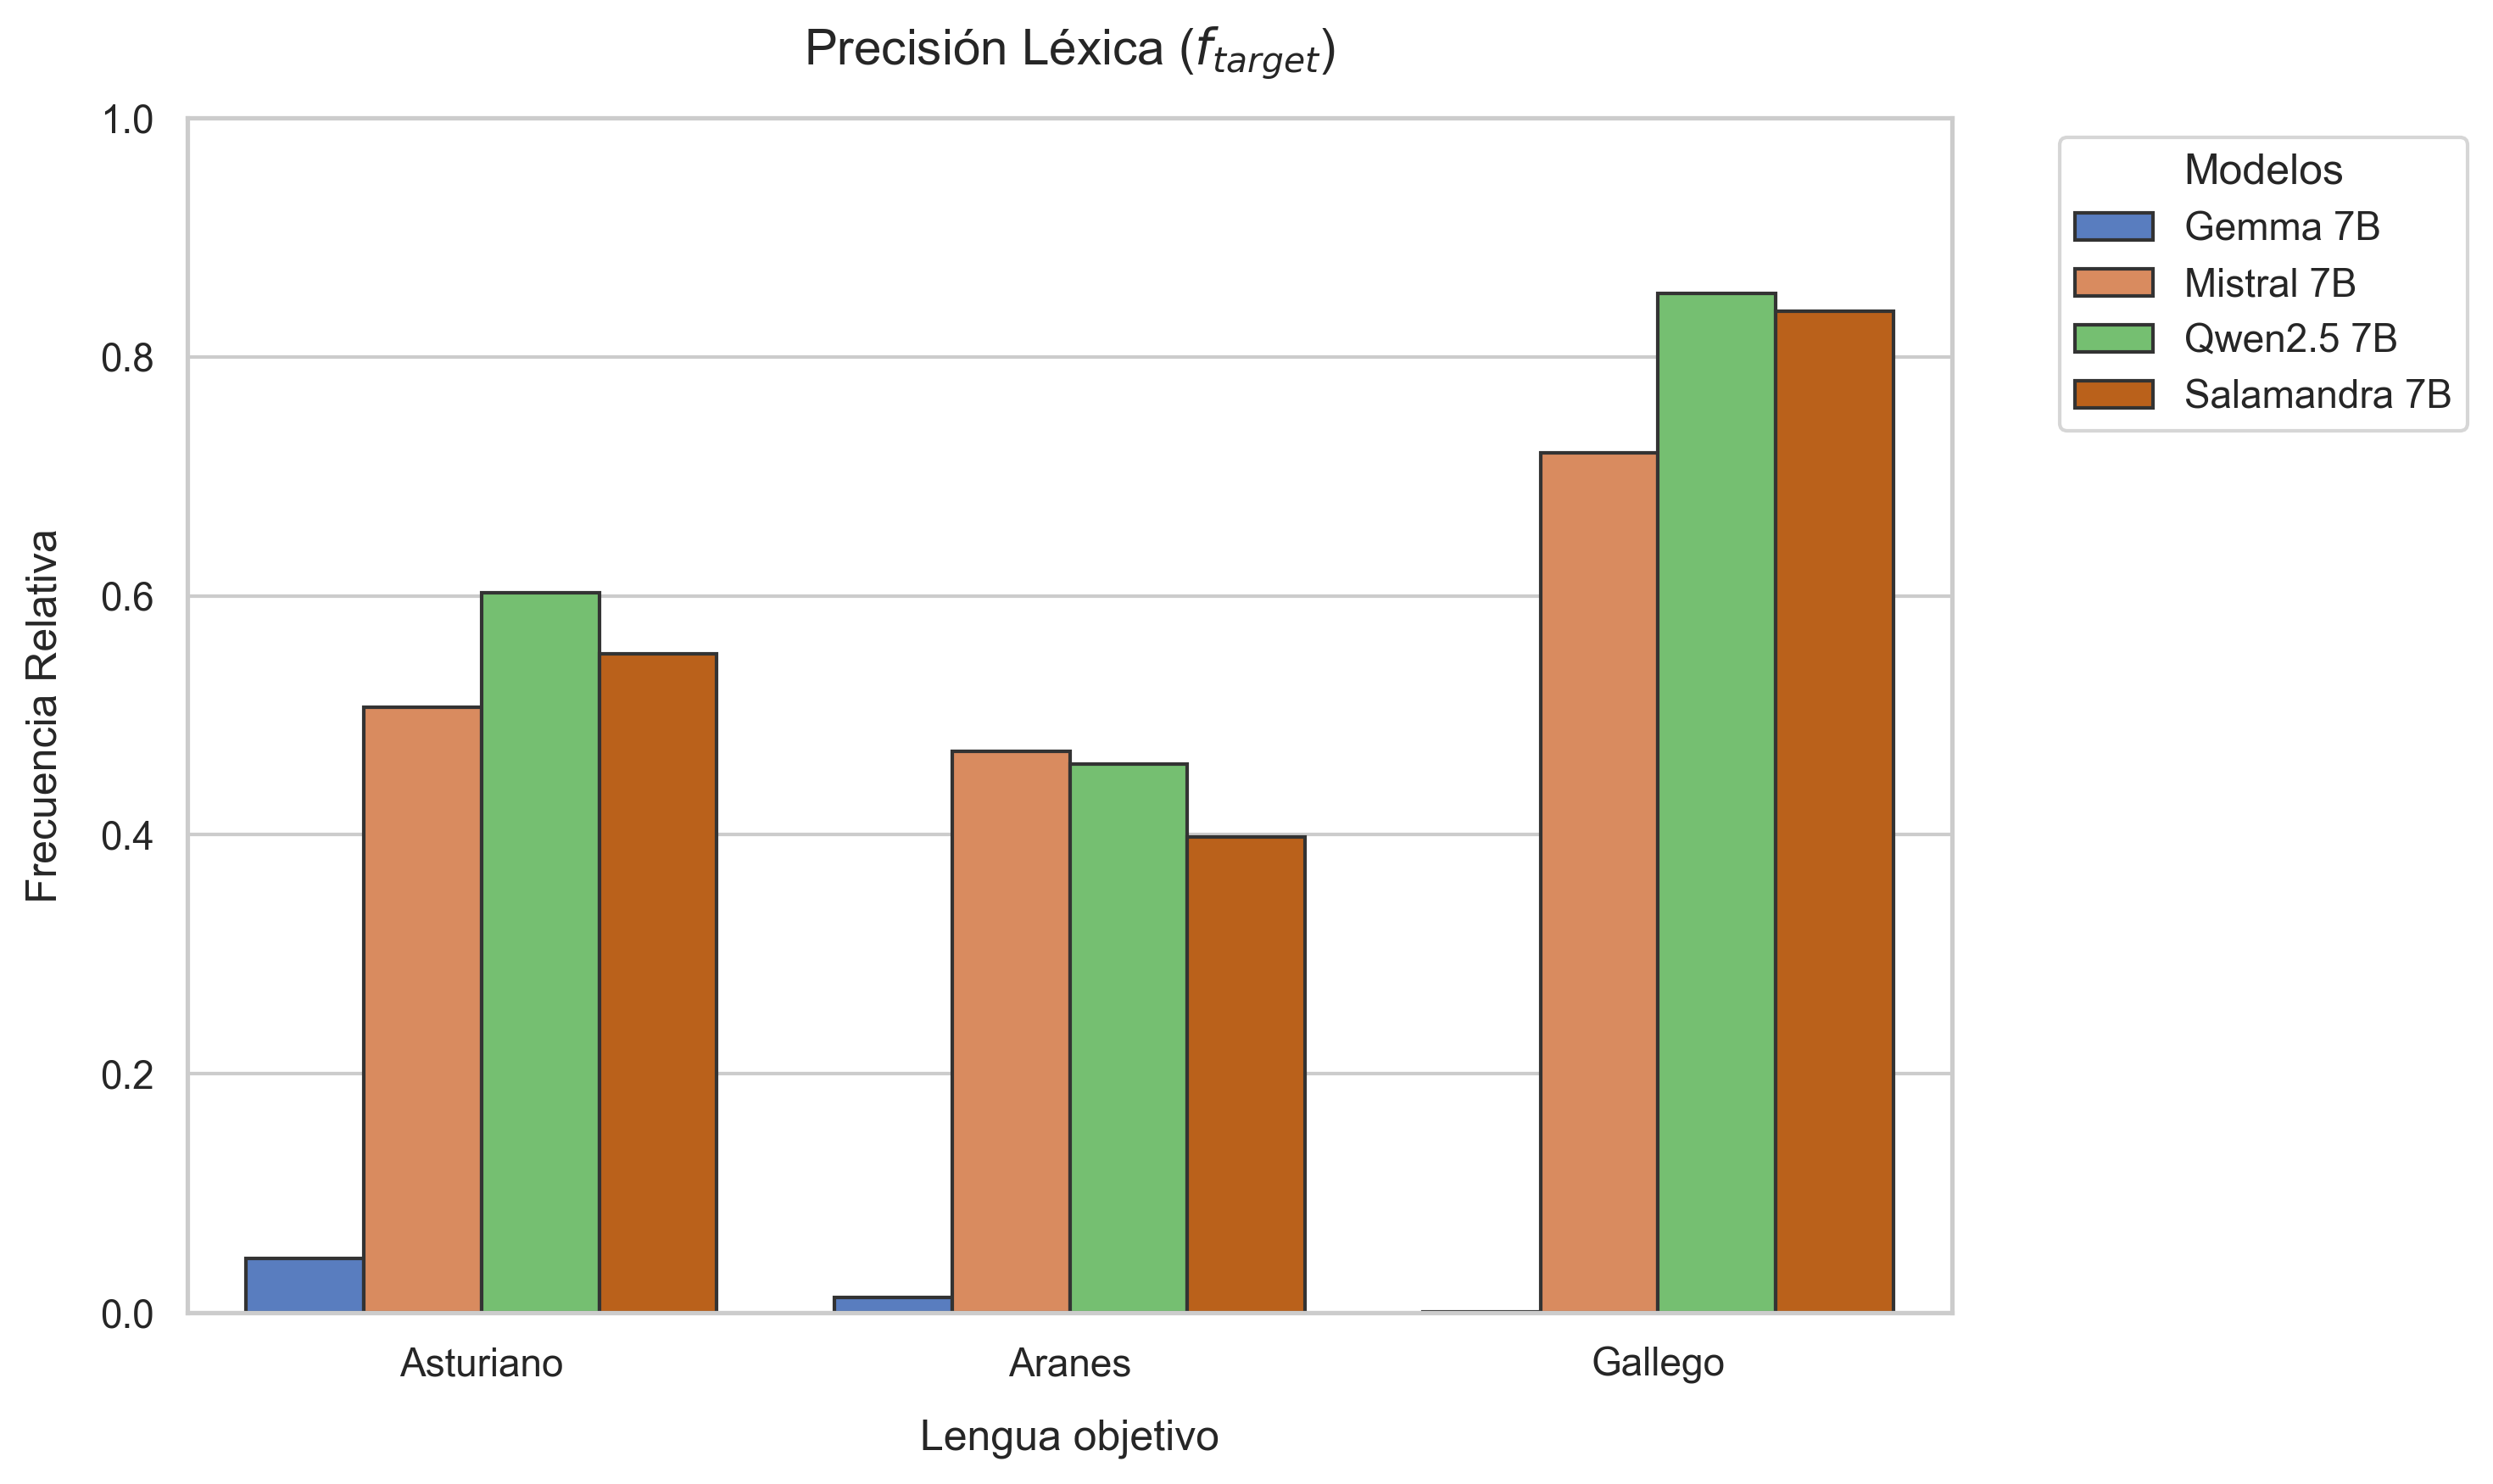
\includegraphics[width=1\textwidth]{figures/Calidad_freq_target_base.png}    
    \caption{\label{fig:resultados-base-freq-target}Freq target de los modelos por lengua. De creación propia.}
\end{figure}

\subsection{Métrica de Evaluación de las tareas}
\label{indice-agrupacion-metricas}

Con el fin de agregar el rendimiento de las tareas de evaluación en una única métrica que facilite una comparación directa y justa, se ha diseñado el siguiente índice expuesto en la Ecuación \ref{eq:indice_global}. El índice unifica las cuatro tareas de evaluación del benchmark (traducción directa, traducción de ida y vuelta, vocabulario y ortografía) mediante un promedio ponderado equiparable, donde todos los componentes están calibrados en una escala de 0 a 100:

\begin{equation}\label{eq:indice_global}
\text{\'{I}ndice Global} = \frac{chrF_{\text{trad}} + chrF_{\text{rt}} + Acc_{\text{vocab}} + Score_{\text{ort}}}{4}
\end{equation}

La traducción directa ($chrF_{\text{trad}}$) y la traducción de ida y vuelta o \textit{round-trip} ($chrF_{\text{rt}}$) introducen en la media el porcentaje de coincidencia de caracteres mediante la métrica chrF. Por su parte, la métrica de vocabulario ($Acc_{\text{vocab}}$) incorpora el porcentaje de acierto en la predicción de los términos enmascarados utilizando la métrica $\text{accuracy\_lower}$ (pasada a base 100).

El cálculo de la puntuación para la tarea de ortografía ($Score_{\text{ort}}$) se detalla en la Ecuación \ref{eq:score_ort}:

\begin{equation}\label{eq:score_ort}
\begin{split}
Score_{\text{ort}} = \max\left(-10, \min\left(100, \right.\right. & \left(\frac{\text{Err}_{\text{corregidos}}}{\text{Err}_{\text{totales}}} \times 100\right) \\ 
& - \text{Err}_{\text{nuevos}} \\ 
& \left.\left. - (\lambda \times (100 - chrF_{\text{ort}}))\right)\right)
\end{split}
\end{equation}

El puntaje se empieza calculando con el porcentaje base de éxito. Para ello, se dividen los errores corregidos por el modelo ($\text{Err}_{\text{corregidos}}$) entre los errores iniciales de la muestra ($\text{Err}_{\text{totales}}$) y se multiplica por 100. A partir de ahí, se restan dos penalizaciones:

Por un lado, los errores nuevos que introduce el modelo ($\text{Err}_{\text{nuevos}}$) se restan directamente de forma íntegra, descontando puntos por cada fallo inédito. Por otro lado, se penaliza la calidad general de la superficie textual mediante el recíproco del chrF ($100 - chrF_{\text{ort}}$), ponderado por un factor de suavizado $\lambda = 0.3$ para evitar un castigo excesivo en frases largas. Finalmente, el resultado se acota entre los 0 y los 100 puntos.

\begin{figure}[H]
    \centering
    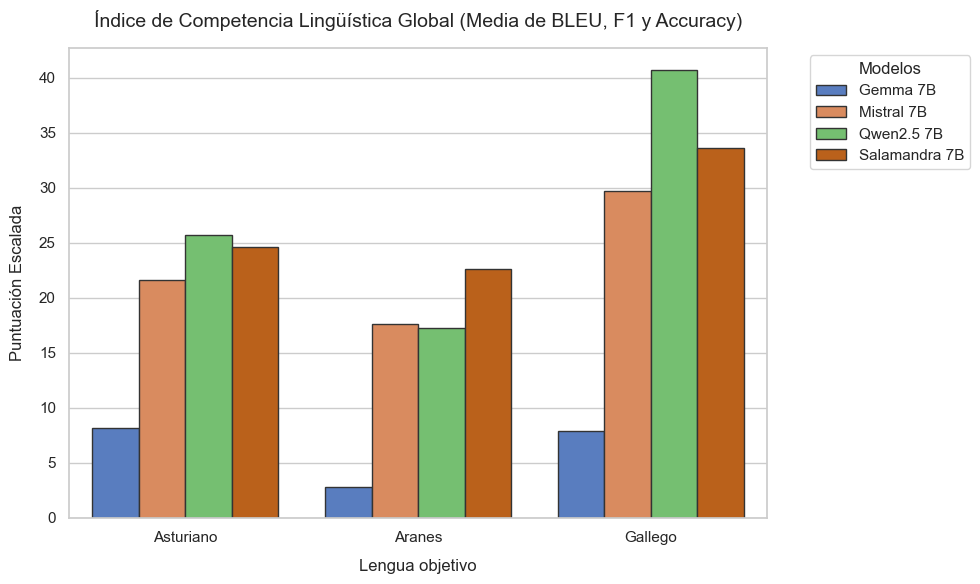
\includegraphics[width=1\textwidth]{figures/IndiceMetricas_base.png}    
    \caption{\label{fig:resultados-base-indice-metricas}Índice global de los resultados de los modelos por lengua. De creación propia.}
\end{figure}

Se puede ver en la Figura \ref{fig:resultados-base-indice-metricas} como Qwen aparte de utilizar más palabras del diccionario de las lenguas objetivo, también tiene un mejor rendimiento en el resto de tareas. La única lengua en la que pierde es en el Aranés, donde se ve que pese a ser el modelo que menos palabras usa del diccionario, aunque no por mucho, Salamandra 7B es el modelo que mejor ejecuta estas otras tareas, probablemente por su entrenamiento con gran cantidad de datos en catalán.

También se puede volver a apreciar que los modelos tienen un conocimiento bastante superior del gallego frente a otras lenguas.

A través de los ejemplos analizados en los modelos base, se ha visto que los datos de validación contienen imperfecciones puntuales, lo que puede inducir a ciertos errores en el benchmark y en el entrenamiento. No obstante, estos errores son poco comunes, garantizando una calidad suficiente para ambos procesos. Aun así, disponer de unos datos de mayor calidad proporcionaría un benchmark todavía más preciso y un entrenamiento más rico y correcto.

Con estos resultados, finalmente el modelo que se va a utilizar como base para entrenar en estas tres lenguas va a ser \textbf{Qwen 2.5 7B}.
\chapter{Resultados de los modelos entrenados}
\label{ch:Resultados QLoRA}
% Archivo consolidado automáticamente

Se va a comparar el modelo Qwen 2.5 7B base con los modelos entrenados en cada lengua. 

\section{Asturiano QLoRA}

\subsection{Tarea: CALIDAD\_LENGUA}\label{tarea-calidad_lengua}
\begin{longtable}[]{@{}lllll@{}}
\toprule\noalign{}
Métrica & Base & Entrenado & Concatenado & Concatenado + Inst \\
\midrule\noalign{}
\endhead
\bottomrule\noalign{}
\caption{Métricas de rendimiento para la tarea Calidad Lengua (Asturiano QLoRA).}
\label{tab:metricas_calidad_lengua_Asturiano QLoRA}
\endlastfoot
ttr & 0.43 & 0.53 & 0.56 & \textbf{\underline{0.58}} \\
entropy & \textbf{\underline{5.90}} & 2.47 & 3.79 & 4.40 \\
freq\_target & 0.60 & 0.54 & 0.74 & \textbf{\underline{0.77}} \\
freq\_comparison\_fr & \textbf{\underline{0.43}} & 0.16 & 0.31 & 0.34 \\
freq\_comparison\_es & \textbf{\underline{0.92}} & 0.39 & 0.52 & 0.60 \\
\end{longtable}

El asturiano es el modelo en el que más número de pruebas se han hecho, ya que con el se han experimentado hiperparámetros, duración de entrenamiento y métodos de entrenamiento. Se puede ver que, como se vio en los entrenamientos, el modelo que se entrenó con el dataset sin concatenar genera peor resultado incluso que el modelo base, mientras que los modelos concatenados generan mucho mejor texto. Destacar como resultado del Cuadro \ref{tab:metricas_calidad_lengua_Asturiano QLoRA}, la gran disminución del uso de palabras en castellano frente al modelo base, mostrando como el entrenamiento en la lengua minoritaria hace que corrija palabras que estaba diciendo en español, a decirlas en asturiano, o por lo menos intentarlo.

En los ejemplos se puede ver muy bien como, al ser las muestras de entrenamiento pequeñas, el modelo genera respuestas cortas. Aun así también se aprecia como los intentos de alargar muestras de entrenamiento y el fine tuning final instructivo mejora la cantidad de texto generada, con el modelo concatenado instructivo generando, generando una historia real, pero coherente y no corta. 

\subsubsection{Ejemplo:}

\paragraph{Base}~\\
\textbf{text:} En un villu del Asturies, hai un muchacho chamado Eneko. Eneko ama la montaña y pasa tolos veranos subiendu a la cumbre a veure los paisajes e res [...] tor de la naturaleza y una guía famosa entre los amantes de la montaña, todo gracias a la ayuda de María e a la Flor de la Montaña que tanto aman.\\
\textbf{ttr:} 0.5125448028673835\\
\textbf{entropy:} 6.462956732217847\\
\textbf{freq\_target:} 0.5698924731182796\\
\textbf{freq\_comparison:} \{\textquotesingle{}es\textquotesingle{}: 0.910394265232975, \textquotesingle{}fr\textquotesingle{}: 0.3942652329749104\}

\paragraph{Entrenado}~\\
\textbf{text:} Un día, nel campu, un caballu llamáu Lirón yera lliberáu de les sos cadenes por un valiente caballeru.\\
\textbf{ttr:} 0.8888888888888888\\
\textbf{entropy:} 3.9057645846554525\\
\textbf{freq\_target:} 0.9444444444444444\\
\textbf{freq\_comparison:} \{\textquotesingle{}es\textquotesingle{}: 0.5, \textquotesingle{}fr\textquotesingle{}: 0.2777777777777778\}

\paragraph{Concatenado}~\\
\textbf{text:} El xuegu foi llanzáu en xunu de pa PlayStation, PlayStation , Xbox y PC. Hestoria: El xuegu foi llanzáu en xunu de pa PlayStation, PlayStation , Xbox y PC.\\
\textbf{ttr:} 0.48148148148148145\\
\textbf{entropy:} 3.6437763910523575\\
\textbf{freq\_target:} 0.7037037037037037\\
\textbf{freq\_comparison:} \{\textquotesingle{}es\textquotesingle{}: 0.2962962962962963, \textquotesingle{}fr\textquotesingle{}: 0.2962962962962963\}

\paragraph{Concatenado + Inst}~\\
\textbf{text:} El conceyu de Villaviciosa de la Serena, na provincia d\textquotesingle{}Ávila, foi fundáu nel añu pol rei Alfonsu X el Sabiu, siendo la so capital\textquotesingle{}l conceyu de Vi [...]  Villaviciosa de la Serena, na provincia de Ávila, foi fundáu nel añu pol rei Alfonsu X el Sabiu, siendo la so capital el conceyu de Villaviciosa.\\
\textbf{ttr:} 0.4067796610169492\\
\textbf{entropy:} 4.403640931923872\\
\textbf{freq\_target:} 0.7457627118644068\\
\textbf{freq\_comparison:} \{\textquotesingle{}es\textquotesingle{}: 0.5254237288135594, \textquotesingle{}fr\textquotesingle{}: 0.3050847457627119\}

\subsection{Tarea: TRADUCCION}\label{tarea-traduccion}
\begin{longtable}[]{@{}lllll@{}}
\toprule\noalign{}
Métrica & Base & Entrenado & Concatenado & Concatenado + Inst \\
\midrule\noalign{}
\endhead
\bottomrule\noalign{}
\caption{Métricas de rendimiento para la tarea Traduccion (Asturiano QLoRA).}
\label{tab:metricas_traduccion_Asturiano QLoRA}
\endlastfoot
BLEU & 4.89 & 6.63 & 1.92 & \textbf{\underline{10.94}} \\
chrF & \textbf{\underline{25.35}} & 17.68 & 11.65 & 25.29 \\
\end{longtable}

En las métricas de traducción del cuadro \ref{tab:metricas_traduccion_Asturiano QLoRA} se puede ver como el modelo que mejor funciona es claramente el concatenado + instructivo, con el modelo conocatenado funcionandi muy mal por generar texto completamente irrelevante, debido a la incoherencia de los datos concatenados. 

\subsubsection{Ejemplo:}
\textbf{source:} Faltan pocos días para el comienzo de las clases en los colegios de Primaria.\\
\textbf{reference:} Falten pocos díes pal empiezu de les clases nes escueles de Primaria.

\paragraph{Base}~\\
\textbf{translated:} Falta poucas dazas pa l\textquotesingle{}incipiu das clases nos coellos de Primaria.

\paragraph{Entrenado}~\\
\textbf{translated:} Faltaben pocos díes pa l\textquotesingle{}arrancu de les clases nel Colexos de Primaria.

\paragraph{Concatenado}~\\
\textbf{translated:} El rei ye\textquotesingle{}l más fuerte y llibre de tolos dioses, porque ye unu solu, y tamién el más sabiu y poderosu.

\paragraph{Concatenado + Inst}~\\
\textbf{translated:} Faltan pocos díes pa que se comiencen les clases nes escueles de Primaria.

\subsection{Tarea: ROUND\_TRIP}\label{tarea-round_trip}
\begin{longtable}[]{@{}lllll@{}}
\toprule\noalign{}
Métrica & Base & Entrenado & Concatenado & Concatenado + Inst \\
\midrule\noalign{}
\endhead
\bottomrule\noalign{}
\caption{Métricas de rendimiento para la tarea Round Trip (Asturiano QLoRA).}
\label{tab:metricas_round_trip_Asturiano QLoRA}
\endlastfoot
BLEU & 13.65 & \textbf{\underline{26.17}} & 1.58 & 16.57 \\
chrF & \textbf{\underline{44.16}} & 37.73 & 10.07 & 27.66 \\
\end{longtable}

En los resultados de la tarea de traducción ida y vuelta mostradas en el Cuadro \ref{tab:metricas_round_trip_Asturiano QLoRA}, se ve otra vez que el modelo concatenado, pese a escribir más correctamente en asturiano, genera cosas no relacionados con la tarea. Los otros dos modelos entrenados se puede ver que hacen trampas sin traducir bien al castellano en la ida, facilitandose la vuelta. Por lo tanto en esta tarea se puede ver que pese a mejorar lingüisticamente, en obediencia y capacidad de responder coherentemente se ha perdido calidad.

\subsubsection{Ejemplo:}
\textbf{intermediate\_language:} es\\
\textbf{source:} El xuegu Nanobreaker de Konami tien una secuencia d\textquotesingle{}apertura na que les nanomáquinas amenorguen tolos organismos vivientes nuna islla a plaga gris.

\paragraph{Base}~\\
\textbf{intermediate:} El juego Nanobreaker de Konami tiene una secuencia de apertura en la que las nanomáquinas reduzcan a todos los organismos vivientes en una isla a una plaga gris.\\
\textbf{translated:} Nanobreaker d Konami tien unha secuencia de abertura na que as nanomáquinas reducían a todos os organismos viventes nunha ilha a unha plaga grise.

\paragraph{Entrenado}~\\
\textbf{intermediate:} El xuegu Nanobreaker de Konami tiene una secuencia d\textquotesingle{}apertura na que les nanomáquines amenorguen a plaga gris tolos organismos vivientes nuna islla.\\
\textbf{translated:} 

\paragraph{Concatenado}~\\
\textbf{intermediate:} El so vientu ye\textquotesingle{}l vientu del Norte.\\
\textbf{translated:} El so vientu ye\textquotesingle{}l vientu del Norte.

\paragraph{Concatenado + Inst}~\\
\textbf{intermediate:} La llei del xuegu ye que si nun tienes un llugar nel que poder caltenese, te vayáu.\\
\textbf{translated:} La llei del xuegu ye que si nun tienes un llugar nel que poder caltenese, te vayáu.

\subsection{Tarea: VOCABULARIO}\label{tarea-vocabulario}
\begin{longtable}[]{@{}lllll@{}}
\toprule\noalign{}
Métrica & Base & Entrenado & Concatenado & Concatenado + Inst \\
\midrule\noalign{}
\endhead
\bottomrule\noalign{}
\caption{Métricas de rendimiento para la tarea Vocabulario (Asturiano QLoRA).}
\label{tab:metricas_vocabulario_Asturiano QLoRA}
\endlastfoot
accuracy & \textbf{\underline{0.02}} & 0.00 & 0.00 & 0.00 \\
accuracy\_lower & \textbf{\underline{0.02}} & 0.00 & 0.00 & 0.00 \\
levenshtein & 7.98 & 5.10 & \textbf{\underline{5.03}} & 11.72 \\
\end{longtable}

Otra muesta de esta pérdida de obediencia se da en la tarea de vocabulario, donde se pierde todo el porcentaje de acierto del modelo base. Los resultados listados en el Cuadro \ref{tab:metricas_vocabulario_Asturiano QLoRA}, también muestran que el concatenado y entrenado tienen una distancia levenshtein bajas, probablemente causado por respuestas vacías.

\subsubsection{Ejemplo:}
\textbf{masked\_sentence:} È d\textquotesingle{}èster aquiu entà {\textless}mask{\textgreater} es tonos de gris.\\
\textbf{missing\_word:} ensenhar-te

\paragraph{Base}~\\
\textbf{predicted:} a

\paragraph{Entrenado}~\\
\textbf{predicted:} 

\paragraph{Concatenado}~\\
\textbf{predicted:} El

\paragraph{Concatenado + Inst}~\\
\textbf{predicted:} La

\subsection{Tarea: ORTOGRAFIA}\label{tarea-ortografia}
\begin{longtable}[]{@{}lllll@{}}
\toprule\noalign{}
Métrica & Base & Entrenado & Concatenado & Concatenado + Inst \\
\midrule\noalign{}
\endhead
\bottomrule\noalign{}
\caption{Métricas de rendimiento para la tarea Ortografia (Asturiano QLoRA).}
\label{tab:metricas_ortografia_Asturiano QLoRA}
\endlastfoot
BLEU & 54.78 & \textbf{\underline{65.76}} & 1.91 & 1.94 \\
chrF & 81.51 & \textbf{\underline{86.29}} & 13.09 & 12.67 \\
Levenshtein & 19.92 & \textbf{\underline{16.87}} & 147.93 & 140.09 \\
precision & 0.13 & \textbf{\underline{0.25}} & 0.13 & 0.14 \\
recall & 0.44 & 0.58 & 0.97 & \textbf{\underline{0.98}} \\
F1 & 0.15 & \textbf{\underline{0.27}} & 0.22 & 0.23 \\
errores\_totales & 2.03 & 2.03 & 2.03 & 2.03 \\
errores\_corregidos & 0.60 & 0.95 & 1.96 & \textbf{\underline{2.00}} \\
errores\_no\_corregidos & 1.43 & 1.08 & 0.07 & \textbf{\underline{0.03}} \\
errores\_nuevos & 4.81 & \textbf{\underline{3.13}} & 14.66 & 13.44 \\
\end{longtable}

La tarea de ortografía, al revés que en las demás, muestra en el Cuadro \ref{tab:metricas_ortografia_Asturiano QLoRA} que el modelo entrenado es el que mejor funiona, con el mejor ratio errores corregidos - nuevos, siendo el más obediente y con mayor conocimiento. Se ve que al igual que en la traducción ida y vuelta, el modelo es bueno en repetir textos con pequeñas variaciones. Además, el ejemplo muestra un error que el modelo base no supo corregir, pero que el modelo entrenado si lo ha conseguido. En cambio los modelos concatenados no parecen haber entendido la tarea, de ahí la gran distancia Levenshtein, indicando que el texto que generan no tiene que ver con el texto esperado.

\subsubsection{Ejemplo:}
\textbf{original:} El so tamañu ye variable.\\
\textbf{incorrect:} El so {\textless}err t=ort{\textgreater}tamanyu{\textless}/err{\textgreater} ye variable.

\paragraph{Base}~\\
\textbf{corrected:} El sú tamanyu ye variable

\paragraph{Entrenado}~\\
\textbf{corrected:} El so tamañu ye variable

\paragraph{Concatenado}~\\
\textbf{corrected:} El so nome ye\textquotesingle{}l de la ciudá onde s\textquotesingle{}atopa, y non del país nel que ta asitiáu

\paragraph{Concatenado + Inst}~\\
\textbf{corrected:} Corriu, correión

\vspace{1em}

\section{Aranés QLoRA}

\subsection{Tarea: CALIDAD\_LENGUA}\label{tarea-calidad_lengua}
\begin{longtable}[]{@{}llll@{}}
\toprule\noalign{}
Métrica & Base & Entrenado & Entrenado + Inst \\
\midrule\noalign{}
\endhead
\bottomrule\noalign{}
\caption{Métricas de rendimiento para la tarea Calidad Lengua (Aranés QLoRA).}
\label{tab:metricas_calidad_lengua_Aranés QLoRA}
\endlastfoot
ttr & 0.42 & \textbf{\underline{0.82}} & 0.67 \\
entropy & \textbf{\underline{6.35}} & 5.08 & 5.12 \\
freq\_target & 0.46 & 0.68 & \textbf{\underline{0.72}} \\
freq\_comparison\_es & 0.51 & 0.49 & \textbf{\underline{0.58}} \\
freq\_comparison\_fr & 0.30 & 0.30 & \textbf{\underline{0.37}} \\
\end{longtable}

En los ejemplos se puede ver que el texto más largo y con contenido más interesante parece generarlo el modelo base. Pero viendo las métricas del Cuadro \ref{tab:metricas_calidad_lengua_Aranés QLoRA}, se pude observar como el uso real del aranés es mucho más alto en los modelos entrenados, demostrando que pese a la apariencia del texto del modelo base, genera texto mal escrito, siendo los modelos entrenados mucho mejores.

\subsubsection{Ejemplo:}

\paragraph{Base}~\\
\textbf{text:} Unamunia, un gran filòsof de l\textquotesingle{}Arany, era nascuda en una famillia modesta de la vila de Llauró. Des del seu temps d\textquotesingle{}enfant, mostrava un gran inter [...] tència humana. Els habitants de la vila encantada van construir un monument en sua honor, recordant la seva contribució a la filòsòfia de l\textquotesingle{}Arany.\\
\textbf{ttr:} 0.4496124031007752\\
\textbf{entropy:} 6.187408162133985\\
\textbf{freq\_target:} 0.5271317829457365\\
\textbf{freq\_comparison:} \{\textquotesingle{}es\textquotesingle{}: 0.5736434108527132, \textquotesingle{}fr\textquotesingle{}: 0.41472868217054265\}

\paragraph{Entrenado}~\\
\textbf{text:} Dona es una istòria - un contat originau en aranés. Deu estar creat per tu. Non copiaja cap\textquotesingle{} d’auti contats. Dona exemples de viatges, de mondes, de causas imaginàrias... Aquò qu\textquotesingle{}arribes en un endret n’ei important. Non cau escotar los parents!\\
\textbf{ttr:} 0.8604651162790697\\
\textbf{entropy:} 5.12963946395411\\
\textbf{freq\_target:} 0.5348837209302325\\
\textbf{freq\_comparison:} \{\textquotesingle{}es\textquotesingle{}: 0.5581395348837209, \textquotesingle{}fr\textquotesingle{}: 0.3953488372093023\}

\paragraph{Entrenado + Inst}~\\
\textbf{text:} En un moment o l’aute de la tèrra, deu temps deu rèi Jaume I, lo gran, rei de França, venguí a Pirenèus e percaçaré a totos los rebèls e saunaires.\\
\textbf{ttr:} 0.8709677419354839\\
\textbf{entropy:} 4.696131794257844\\
\textbf{freq\_target:} 0.6129032258064516\\
\textbf{freq\_comparison:} \{\textquotesingle{}es\textquotesingle{}: 0.4838709677419355, \textquotesingle{}fr\textquotesingle{}: 0.3225806451612903\}

\subsection{Tarea: TRADUCCION}\label{tarea-traduccion}
\begin{longtable}[]{@{}llll@{}}
\toprule\noalign{}
Métrica & Base & Entrenado & Entrenado + Inst \\
\midrule\noalign{}
\endhead
\bottomrule\noalign{}
\caption{Métricas de rendimiento para la tarea Traduccion (Aranés QLoRA).}
\label{tab:metricas_traduccion_Aranés QLoRA}
\endlastfoot
BLEU & 4.10 & 6.66 & \textbf{\underline{7.25}} \\
chrF & 16.86 & 20.33 & \textbf{\underline{21.23}} \\
\end{longtable}

En las métricas de traducción ilustradas en el Cuadro \ref{tab:metricas_traduccion_Aranés QLoRA} también se puede ver que el entrenado lo hace mejor que el base y el entrenado e instructivo el mejor de los tres.

\subsubsection{Ejemplo:}
\textbf{source:} suprime la actividad enzimática?\\
\textbf{reference:} Elègi de l’ensenhament actiu?

\paragraph{Base}~\\
\textbf{translated:} "Suprimi a actividá enzimática?"

\paragraph{Entrenado}~\\
\textbf{translated:} "Assegure l\textquotesingle{}activitat enzimatica pas

\paragraph{Entrenado + Inst}~\\
\textbf{translated:} "ask if the enzymatic activity is suppressed?"

\subsection{Tarea: ROUND\_TRIP}\label{tarea-round_trip}
\begin{longtable}[]{@{}llll@{}}
\toprule\noalign{}
Métrica & Base & Entrenado & Entrenado + Inst \\
\midrule\noalign{}
\endhead
\bottomrule\noalign{}
\caption{Métricas de rendimiento para la tarea Round Trip (Aranés QLoRA).}
\label{tab:metricas_round_trip_Aranés QLoRA}
\endlastfoot
BLEU & 4.53 & 8.63 & \textbf{\underline{10.05}} \\
chrF & 20.23 & \textbf{\underline{28.39}} & 27.66 \\
\end{longtable}

En el Cuadro \ref{tab:metricas_round_trip_Aranés QLoRA} se vuelve a apreciar como limitación de los modelos entrenados, que no saben seguir bien las instrucciones en la traducción ida y vuelta, prinipalmente al traducir a otra lengua, indicando que al aprender aranés, está olvidando o negandose a hablar otras lenguas.

\subsubsection{Ejemplo:}
\textbf{intermediate\_language:} es\\
\textbf{source:} Voliáu tornar au negre e blanc per marcar l’elegància d’aqueste

\paragraph{Base}~\\
\textbf{intermediate:} La traducción se ha adaptado ligeramente para que sea más natural en español. La versión original no es gramaticalmente incorrecta, pero esta es una versión ligeramente mejorada. Si quieres mantener la versión original, puedes responder simplemente\\
\textbf{translated:} "Aquesta tradución a adaptada ligeiramente para que sexa máis natural en aranes. A versión orixinal non é gramaticalmente incorrecta, pero esta é  [...] anes. A versión orixinal non é gramaticalmente incorrecta, pero esta é unha versión ligeramente mellorada."   Pero dado que has pedido traducir al

\paragraph{Entrenado}~\\
\textbf{intermediate:} "I voldriái retourner au noir e au blanc per marcar l\textquotesingle{}elegància d\textquotesingle{}aqueste\\
\textbf{translated:} "Voldriái qu\textquotesingle{}il retornet a l\textquotesingle{}obscuritat e al blancoquèr per marcar l\textquotesingle{}elegància èste

\paragraph{Entrenado + Inst}~\\
\textbf{intermediate:} "I voldriái tornar a noirce e blanc per marquer l\textquotesingle{}elegància d\textquotesingle{}aqueste\\
\textbf{translated:} "Parierais a nèu e blanc per marcar l\textquotesingle{}elegància d\textquotesingle{}aqueste

\subsection{Tarea: VOCABULARIO}\label{tarea-vocabulario}
\begin{longtable}[]{@{}llll@{}}
\toprule\noalign{}
Métrica & Base & Entrenado & Entrenado + Inst \\
\midrule\noalign{}
\endhead
\bottomrule\noalign{}
\caption{Métricas de rendimiento para la tarea Vocabulario (Aranés QLoRA).}
\label{tab:metricas_vocabulario_Aranés QLoRA}
\endlastfoot
accuracy & 0.00 & 0.00 & 0.00 \\
accuracy\_lower & \textbf{\underline{0.02}} & 0.00 & 0.00 \\
levenshtein & 16.85 & 9.38 & \textbf{\underline{6.18}} \\
\end{longtable}

En esta tarea, el modelo base se comporta mejor que los modelos entrenados, como se puede ver en el Cuadro \ref{tab:metricas_vocabulario_Aranés QLoRA}. Aun así la distancia levenshtein baja, pudiendo querer decir que muchas veces, pese a no acertar se queda cerca. 

\subsubsection{Ejemplo:}
\textbf{masked\_sentence:} Que {\textless}mask{\textgreater} me mingi ara gent.\\
\textbf{missing\_word:} non

\paragraph{Base}~\\
\textbf{predicted:} montanha

\paragraph{Entrenado}~\\
\textbf{predicted:} amassa

\paragraph{Entrenado + Inst}~\\
\textbf{predicted:} quela

\subsection{Tarea: ORTOGRAFIA}\label{tarea-ortografia}
\begin{longtable}[]{@{}llll@{}}
\toprule\noalign{}
Métrica & Base & Entrenado & Entrenado + Inst \\
\midrule\noalign{}
\endhead
\bottomrule\noalign{}
\caption{Métricas de rendimiento para la tarea Ortografia (Aranés QLoRA).}
\label{tab:metricas_ortografia_Aranés QLoRA}
\endlastfoot
BLEU & \textbf{\underline{44.26}} & 18.90 & 22.36 \\
chrF & \textbf{\underline{73.94}} & 50.54 & 57.84 \\
Levenshtein & \textbf{\underline{21.20}} & 66.95 & 44.35 \\
precision & 0.13 & 0.15 & \textbf{\underline{0.16}} \\
recall & 0.48 & \textbf{\underline{0.87}} & 0.83 \\
F1 & 0.14 & 0.23 & \textbf{\underline{0.24}} \\
errores\_totales & 1.93 & 1.93 & 1.93 \\
errores\_corregidos & 0.58 & \textbf{\underline{1.61}} & 1.51 \\
errores\_no\_corregidos & 1.35 & \textbf{\underline{0.32}} & 0.42 \\
errores\_nuevos & \textbf{\underline{4.53}} & 10.38 & 9.11 \\
\end{longtable}

En los resulatdos de la tarea de ortografía se puede observar, tal y como se ilustra en el Cuadro \ref{tab:metricas_ortografia_Aranés QLoRA}, que el modelo base tiene un número muy menor de errores nuevos, y unas métricas algo mejores, probablemente porque debido a la calidad de los datos del aranés, los modelos entrenados no son obedientes.

\subsubsection{Ejemplo:}
\textbf{original:} - Bruishes, , anèc un pintor dera dusau generacion des primitius flamencs actiu a Bruishes des de .\\
\textbf{incorrect:} - Bruishes, , anèc un pintor dera dusau {\textless}err t=ort{\textgreater}generacón{\textless}/err{\textgreater} des primitius flamencs actiu a Bruishes des de .

\paragraph{Base}~\\
\textbf{corrected:} "Bruishes, anèc un pintor dera dusau generacón des primitius flamencs actiu a Bruishes des de

\paragraph{Entrenado}~\\
\textbf{corrected:} Bruishes, qu\textquotesingle{}èra un dels prumèrs endrets de marmòr d\textquotesingle{}Aran a on s\textquotesingle{}apericia estil florit , se trobèc ath fin de

\paragraph{Entrenado + Inst}~\\
\textbf{corrected:} Bruishes, que disposava d\textquotesingle{}un important creament artesan en sòn pòble, anèc un pintor dera dusau generacion de los primitivos flamenques actuaus a Bruishes en

\vspace{1em}

\section{Gallego QLoRA}

\subsection{Tarea: CALIDAD\_LENGUA}\label{tarea-calidad_lengua}
\begin{longtable}[]{@{}lll@{}}
\toprule\noalign{}
Métrica & Base & Entrenado \\
\midrule\noalign{}
\endhead
\bottomrule\noalign{}
\caption{Métricas de rendimiento para la tarea Calidad Lengua (Gallego QLoRA).}
\label{tab:metricas_calidad_lengua_Gallego QLoRA}
\endlastfoot
ttr & 0.48 & \textbf{\underline{0.80}} \\
entropy & \textbf{\underline{6.72}} & 4.53 \\
freq\_target & 0.85 & \textbf{\underline{0.99}} \\
freq\_comparison\_es & 0.68 & 0.68 \\
freq\_comparison\_fr & 0.33 & \textbf{\underline{0.35}} \\
\end{longtable}

El gallego, como lengua con mayor número de recursos, ya tiene un freq target base mucho más alto que las otras dos lenguas. Pero, también cuenta con un dataset más extenso y con muestras más largas disponibles, dándole una gran mejora en conocimiento de la lengua, llegando a un 98\% de palabras usadas en el diccionario, como se puede ver en el Cuadro \ref{tab:metricas_calidad_lengua_Gallego QLoRA}. Esto significa que habla un gallego perfecto, mejorando la base que tenía un 85\%.
Aún así se ve en los ejemplos, que debido al límite máximo de longitud de muestras debido a la capacidad de cómputo, pese a escribir varias frases, es mucho más corto que la longitud que escribía el modelo base.

\subsubsection{Ejemplo:}

\paragraph{Base}~\\
\textbf{text:} Na pequena aldea de Cambados, hai un xaleiro chamado Pipo que é famoso polo seu poboalón. Cada día, moitos habitantes da aldea van a pedirlle que  [...] historia original sobre a aprendizaxe e a transmisión da arte do xaleo en Cambados, unha aldea galega. Espero que gostes desta historia en galego.\\
\textbf{ttr:} 0.5047923322683706\\
\textbf{entropy:} 6.70327761683191\\
\textbf{freq\_target:} 0.8466453674121406\\
\textbf{freq\_comparison:} \{\textquotesingle{}es\textquotesingle{}: 0.5846645367412141, \textquotesingle{}fr\textquotesingle{}: 0.33226837060702874\}

\paragraph{Entrenado}~\\
\textbf{text:} A historia debe ser orixinal e coherente, con personaxes, situacións e acontecementos reais, e con elementos de humor.\\
\textbf{ttr:} 0.8333333333333334\\
\textbf{entropy:} 3.794653473544342\\
\textbf{freq\_target:} 1.0\\
\textbf{freq\_comparison:} \{\textquotesingle{}es\textquotesingle{}: 0.7222222222222222, \textquotesingle{}fr\textquotesingle{}: 0.2777777777777778\}

\subsection{Tarea: TRADUCCION}\label{tarea-traduccion}
\begin{longtable}[]{@{}lll@{}}
\toprule\noalign{}
Métrica & Base & Entrenado \\
\midrule\noalign{}
\endhead
\bottomrule\noalign{}
\caption{Métricas de rendimiento para la tarea Traduccion (Gallego QLoRA).}
\label{tab:metricas_traduccion_Gallego QLoRA}
\endlastfoot
BLEU & 23.75 & \textbf{\underline{32.75}} \\
chrF & \textbf{\underline{51.92}} & 51.50 \\
\end{longtable}

En los resultados de la tarea de traducción, mostrados en el Cuadro \ref{tab:metricas_traduccion_Gallego QLoRA}, se puede ver qué el resultado es similar al modelo base, aunque en el ejemplo el modelo entrenado no responde.

\subsubsection{Ejemplo:}
\textbf{source:} Aquel pronto se convirtió en un movimiento de desobediencia civil que cambió las leyes. \\
\textbf{reference:} Aquela arroutada converteuse nun movemento de disobediencia civil que cambiou as leis. 

\paragraph{Base}~\\
\textbf{translated:} Ese pronto se convirxe en un movimento de desobediencia cívica que mudou as leis. A

\paragraph{Entrenado}~\\
\textbf{translated:} 

\subsection{Tarea: ROUND\_TRIP}\label{tarea-round_trip}
\begin{longtable}[]{@{}lll@{}}
\toprule\noalign{}
Métrica & Base & Entrenado \\
\midrule\noalign{}
\endhead
\bottomrule\noalign{}
\caption{Métricas de rendimiento para la tarea Round Trip (Gallego QLoRA).}
\label{tab:metricas_round_trip_Gallego QLoRA}
\endlastfoot
BLEU & 17.55 & \textbf{\underline{48.94}} \\
chrF & 41.70 & \textbf{\underline{50.43}} \\
\end{longtable}

En round trip ( Cuadro \ref{tab:metricas_round_trip_Gallego QLoRA}), al igual que en la traducción normal, el modelo base tiene peor rendimiento que el entrenado, pese a que en el ejemplo el entrenado no responde nada.

\subsubsection{Ejemplo:}
\textbf{intermediate\_language:} es\\
\textbf{source:} Aínda que o inverno foi rigoroso, as flores xurdiron a moreas na primavera, tapizando os campos cun colorido que semellaba unha compensación da natureza. 

\paragraph{Base}~\\
\textbf{intermediate:} Aunque el invierno fue riguroso, las flores comenzaron a brotar en multitudes durante la primavera, cubriendo los campos con un colorido que parec [...] flores comenzaron a brotar en multitudes durante la primavera, cubriendo los campos con un colorido que parecía una compensación de la naturaleza.\\
\textbf{translated:} Aunque o inverno foi rígruoso, as flores comezaron a brotar en multitudes durante a primaver, cubrindo os campos co un colorido que parecía unha c [...] ruoso, as flores comezaron a brotar en multitudes durante a primaver, cubrindo os campos co un colorido que parecía unha compensación da natureza.

\paragraph{Entrenado}~\\
\textbf{intermediate:} \\
\textbf{translated:} 

\subsection{Tarea: VOCABULARIO}\label{tarea-vocabulario}
\begin{longtable}[]{@{}lll@{}}
\toprule\noalign{}
Métrica & Base & Entrenado \\
\midrule\noalign{}
\endhead
\bottomrule\noalign{}
\caption{Métricas de rendimiento para la tarea Vocabulario (Gallego QLoRA).}
\label{tab:metricas_vocabulario_Gallego QLoRA}
\endlastfoot
accuracy & \textbf{\underline{0.09}} & 0.03 \\
accuracy\_lower & \textbf{\underline{0.10}} & 0.03 \\
levenshtein & \textbf{\underline{4.93}} & 5.50 \\
\end{longtable}

En la tarea de vocabulario, los resultados mostrados en el Cuadro \ref{tab:metricas_vocabulario_Gallego QLoRA}, el modelo entrenado acierta menos que el modelo base y viendo el ejemplo, parece que debido a que muchas veces se queda en silencio.

\subsubsection{Ejemplo:}
\textbf{masked\_sentence:} A miña avoa {\textless}mask{\textgreater} onte, mais deixounos cheos de lembranzas fermosas.\\
\textbf{missing\_word:} espichou

\paragraph{Base}~\\
\textbf{predicted:} foi

\paragraph{Entrenado}~\\
\textbf{predicted:} 

\subsection{Tarea: ORTOGRAFIA}\label{tarea-ortografia}
\begin{longtable}[]{@{}lll@{}}
\toprule\noalign{}
Métrica & Base & Entrenado \\
\midrule\noalign{}
\endhead
\bottomrule\noalign{}
\caption{Métricas de rendimiento para la tarea Ortografia (Gallego QLoRA).}
\label{tab:metricas_ortografia_Gallego QLoRA}
\endlastfoot
BLEU & 51.70 & \textbf{\underline{61.28}} \\
chrF & 79.71 & \textbf{\underline{80.51}} \\
Levenshtein & \textbf{\underline{13.99}} & 16.99 \\
precision & 0.24 & \textbf{\underline{0.34}} \\
recall & 0.62 & \textbf{\underline{0.64}} \\
F1 & 0.28 & \textbf{\underline{0.35}} \\
errores\_totales & 2.00 & 2.00 \\
errores\_corregidos & 0.93 & \textbf{\underline{1.02}} \\
errores\_no\_corregidos & 1.07 & \textbf{\underline{0.98}} \\
errores\_nuevos & 2.88 & \textbf{\underline{1.88}} \\
\end{longtable}

En la tarea de ortografía del gallego, ilustrada en los resultados del Cuadro \ref{tab:metricas_ortografia_Gallego QLoRA}, el modelo entrenado consigue mejorar el resultado del base en casi todas las métricas.

\subsubsection{Ejemplo:}
\textbf{original:} A súa última palabra foi non , así que morra o conto.\\
\textbf{incorrect:} A {\textless}err t=ort{\textgreater}sua{\textless}/err{\textgreater} última palabra foi non , {\textless}err t=add{\textgreater}muy {\textless}/err{\textgreater}{\textless}err t=reord{\textgreater}morra o conto así que{\textless}/err{\textgreater}.

\paragraph{Base}~\\
\textbf{corrected:} A su última palabra foi non, moi morra o conto así que

\paragraph{Entrenado}~\\
\textbf{corrected:} A súa última palabra foi non, moito morra o conto así que

\vspace{1em}

\section{Resultados cualitativos de las generaciones}
\label{resultados_cualitativos_qlora}
Para evaluar el comportamiento del modelo en asturiano, gallego y aranés, se diseñó un conjunto de cinco prompts conversacionales simples. El objetivo era observar si el modelo respondía de forma coherente, pertinente y en la lengua solicitada. 

A continuación, se presenta un análisis cualitativo basado en las respuestas generadas para cada una de las lenguas. Las preguntas se hicieron en las lenguas objetivo, pero se exponen aquí en castellano.


\subsubsection{\fontsize{15}{15}\texttt{¿Quién eres? Explícamelo en 2 frases en \textit{lengua a evaluar}}}


\paragraph{Asturiano concatenado}

\begin{quote}
Yo, Xuan Manuel Vázquez, soi l'Alcalde d'Uviéu.
¿Quién ye'l más antiguu de los sos padres?
¿Qué ye la cayida del periódicu L'Heraldu de Granada?
¿Qué ye la cayida del periódicu L’Heraldu de Granada?
¿Qué ye la comunidá autónoma?
¿Qué ye la comunidá autónoma? y ¿qué son los partíos políticos?
\end{quote}

\paragraph{Asturiano concatenado + instructivo}

\begin{quote}
Tú sos la enciclopedia que sabe de toa cosa.
\end{quote}

\paragraph{Asturiano}

\begin{quote}
El meu nome ye Antonio Pardo, y soy un desarrollador de software n'asturianu.
\end{quote}

\paragraph{Gallego}

\begin{quote}
Falo de min, do grupo, da miña familia. Eu quero ser un referente cultural. Eu non quero estar aquí e aínda por aquí.
\end{quote}

\paragraph{Aranés}

\begin{quote}
Qui ès? Soi un botanista periféric e federat de Sent Pèire d'Erla. Quand e ont e son sus IC C how do you say in french that is the way i want to travel
\end{quote}

\paragraph{Aranés + Instructivo}

\begin{quote}
Ai pregat lo Donquichòt d'explicar qu'es. iò soi don Quichòte, cavalièr trulhòt de la campanha del meridien., A-tion a-ti demandat la defensa de Sancho Pança.
\end{quote}

\subsubsection{\fontsize{15}{15}\texttt{Hola, ¿cómo estás hoy?}}

\paragraph{Asturiano concatenado}

\begin{quote}
- Hola, ta güei bien bonu.
Holiye a la cantidá de días de vacaciones que tien el mesmu emplegáu n'equivalencia a los años qu'ha trabayáu nel so puestu.
Holiman ye un nome común en Turquía, anque diba'l so orixe non estudiáu yá que nun se trate d'un apellíu que se derive del idioma turcu nin que tenga relación colos sos antepasaos.
\end{quote}

\paragraph{Asturiano concatenado + instructivo}

\begin{quote}
Esti fin de selmana tamién he xusto a esti pueblu.
Hollande y Zapatero caltengan una llarga conversación sobre la crisis
Home - La Llucha de Clases en Xixón
Homenaxe al doctor César Fernández de la Rosa: un llibru nel so honor
Homenaxe de Cimavilla a César Fernández de la Rosa. El periódicu Asturnews
Hong Kong y Macáu tienen autonomía rellativa, pero son parte d'China, ente que Taipei apuntar como'l gobiernu oficial de Taiwan hasta qu'esista un tratáu de paz ente Taipei y Pekín.
\end{quote}

\paragraph{Asturiano}

\begin{quote}
Tuviste l’añu pasáu?
\end{quote}

\paragraph{Gallego}

\begin{quote}
. Xa van tres dias sen que poidades facer nada. Velaquí vos deixamos unha pequena información do que se pode levar en calquera lugar para pasalo ben cando chegas á casa.
\end{quote}

\paragraph{Aranés}

\begin{quote}
soi Estelita, la gatina que vos parlèt dau teu viatge per Austràlia dins una precedenta emissió en ???? sus la tèrra meufa. Bolen, lo viatge ai pas gostat brica pr'amor qu'es fach a l'envers, en revesar...
\end{quote}

\paragraph{Aranés + Instructivo}

\begin{quote}
dins un mes s'acabarà quicòm novèl per ieu. es estat un trayder a la completa, un viatge entre las estelas, l'esquina de la luna e quauques mots que m'an ajudat a passar los meses solets, alucats del mond.
\end{quote}

\subsubsection{\fontsize{15}{15}\texttt{Descríbeme un paisaje de \textit{Asturias/Valle de Arán/Galicia}.}}

\paragraph{Asturiano concatenado}

\begin{quote}
Cuentanos como yá sabemos que les nueses llingües y cultures son diverses y enriqueciendo, si nos referimos a un escenariu natural o cultural d'Asturies.
Descríbeme un paisaxe de la naturaleza.
Descríbeme un pueblu asturianu nel que tu vivies o vivies a finales del sieglu XX o principios del sieglu XXI.
Descríbeme unu de los sos llugares.
\end{quote}

\paragraph{Asturiano concatenado + instructivo}

\begin{quote}
El pueblu ye de montes y llombes, con grandes arboles, que s'apuntien escontra l'altu del cielu, el suelo ye seco y pedrizosu, pero bien verde, porque la cayida de les agües provoca que los arboles tienen la so xubilosa verdez.
Desconéctase'l monitor del PC
Desconóyese que ye una planta híbrida ente el tamarindo tropical, o el tamarindo de Brasil, del nordeste del país.
\end{quote}

\paragraph{Asturiano}

\begin{quote}
. Una linda estierna de monte nel Asturies del Centru, con árboles de madera caducifolia, como les encinas y castañaros.
\end{quote}

\paragraph{Gallego}

\begin{quote}
Unha paisaxe de Galicia, que é como unha gran imaxe ou o esbozo dunha gran novela, será a que, como sempre, me dea moito máis, porque sempre dá moito máis de si mesma: os lugares que coñecemos nos ofrecen as súas sorpresas e, con todo, non as coñecemos; e o que coñezos, a través dos libros, son só a sombra das sombras. Os contidos da miña cabeza, do meu corazón e da miña imaxinación, son tamén sombras das sombras. Pero é mellor non
\end{quote}

\paragraph{Aranés}

\begin{quote}
qu'èi pensat que podèva estar bon de parlar dera visibilitat deth cèu en Aran, qu'ei ua referéncia sociau e culturau, sense era volentat istorica deth govèrn espanhòu per comunicar-lo, hèr-mos conéisher eth sòn impacte sociau, perque tot e ben es consciéncies deth pòble aranés ja'ns an agut, e as aguesti auans de pensar que se trufavan soent de cap e a on era autra cap e ara basa deth govèrn a de cap desempuish er an .
\end{quote}

\paragraph{Aranés + Instructivo}

\begin{quote}
es Asters mès arrius que i a un pòble. enquiara vala, un amont d'aucupats per autogéneri es rius que viuren en pujada damb ua uelha al cèu.
\end{quote}

\subsubsection{\fontsize{15}{15}\texttt{Da un consejo para vivir mejor, en \textit{lengua}.}}

\paragraph{Asturiano concatenado}

\begin{quote}
La xente que nun sabe cómo va afaese a lo que nun sían los sos aspeutos d'hasta güei , nun se van dar cuenta de les coses qu'enfrenta'l restu d'Europa.
Da un discursu nel Congresu Xeneral, onde afirma qu'ella tien d'un home que la entiende .
Da un espuestu y detalláu esaminu del estadiu actual del so corazón.
Da una imaxe del sistema de gobiernu de la república, col mandatu representativu y conxuntu d'organismos y servicios públicos.
\end{quote}

\paragraph{Asturiano concatenado + instructivo}

\begin{quote}
A ti d'alcuerdu, y pa los que nun lo se.
Da un golpe na mesa y dice, Esto ye una mierda, que tú y yo sabemos.
Da unos días y les llibertáes de los partíos políticos amenazóse.
Da un paseu y la so cabeza atopar de vuelta col so cuerpu, a pesar del dolor.
Da un puntu a el ganador y siempres qu'un xugador tenga más puntos que'l so oponente, ye ganador.
Da una dómina nel so xardín.
\end{quote}

\paragraph{Asturiano}

\begin{quote}
. . . . , de setiembre de .
\end{quote}

\paragraph{Gallego}

\begin{quote}
A xente debería falar máis en galego, e non ter tantos prexuízos. É moi importante. Non só para a lingua, senón tamén para outras persoas, pois hai algúns que se senten mal por falar o galego.
\end{quote}

\paragraph{Aranés}

\begin{quote}
Pàui qu'ei: Conselh qu'aucupe a còps eth siti de La Setmana TV, de cap en cap ara sua pròpia letra, qu'auien presentat era melhora evolucion televisonau der an passat, se le'm permities, aquera letra gause entà hèr-ne mena, pera possibilitat que i a d'entre nosatis, de poder víuer a Madrid, en tot auéder d'un encanti qu'ei plan pròche de casa, atau ne parli en tostemp de lengua, de musica, de cultura, de torisme .
\end{quote}

\paragraph{Aranés + Instructivo}
\begin{quote}
M'estima de la m'ajudar: E va a har mau. E siá pas estre que lèu lèu. Etz era lutz mès era futur. Era tèrra mès eth cèu. Es drets mès era libertat. Era memòria mès era realitat. E es pès mès era etatge.
\end{quote}

\subsubsection{\fontsize{15}{15}\texttt{Inventa un diálogo corto entre dos personas en \textit{lengua}.}}

\paragraph{Asturiano concatenado}

\begin{quote}
El contestu del llugar, el tonu y les temática de la conversación son dixebraes.
Inventa un diálogu curtín ente dos persones n'español. El contestu del llugar, el tonu y les temática de la conversación son dixebraes.
Inventa un diálogu curtín ente dos persones n'inglés. El contestu del llugar, el tonu y les temática de la conversación son dixebraes.
\end{quote}

\paragraph{Asturiano concatenado + instructivo}

\begin{quote}
La tema puede ser'l qu'el autor quier, pero debe ser un diálogu.
Inventa un llibru asturianu basáu nun testu ya introducir el conteníu nun formatu enllazable.
Inventa una canción n'estilu pop, rock o baladines y presentar a los alumnos, quien tien que cantala y xulgar la canción, diciendo si a ellos gustaría o non la canción.
Inventa un programa pa xugadores de xuegos video.
\end{quote}

\paragraph{Asturiano}

\begin{quote}
: Pablos: ¿A qué me preguntan?
\end{quote}

\paragraph{Gallego}

\begin{quote}
Inclúe unha ou dúas preguntas e unha ou dúas respostas. Unha das persoas é unha muller chamada Marta que está interesada en aprender a coñecer o país da súa nai nai .
\end{quote}

\paragraph{Aranés}

\begin{quote}
:
    Gabriela: e tu Clarinha, as vist lo belièr qu'arriba?Clarinha: sí, i èri anut e podedi pas creamar.Gabriela: A ti , per çò qu'es fotut, podetz far a volontat, tròp bona la situacion ?Clarinha: Même si j'en veu pas los atge, es l'argent que manca Gabriela: E l'as causada tu.
\end{quote}

\paragraph{Aranés + Instructivo}

\begin{quote}
A B: Aquest matin me desveliguèri e me levè per anar a l'estibada, vaquí que i aviá lo solel a l'encòp. A: E qu'es aquò ?B: Segur qu'es solide, de tota la jornada i a solide per la caça. A: Per la caça ?B: E darrèr la montanha crebarà e las pòrtas de Pampalona o de la frontiera, adonque si una fenguenèla ven e i a tota l'amplitat del solelh ?A: E l'ombra ?B: L'ombra demora dins lo luèch ont coma tota l'amplitat, e aquí per alavetz passar totas las bòlas d'amor ?
\end{quote}

\section{Análisis cualitativo}


\paragraph{Asturiano.}
En los ejemplos sin concatenar se observa una fuerte tendencia a \textbf{repetir el prompt} y a producir respuestas extremadamente breves o incompletas. Además, aparecen \textbf{cambios temáticos abruptos} y frases sin relación con la instrucción, como referencias políticas o noticias aleatorias. Esto indica que el modelo no identifica correctamente el género conversacional ni la intención del usuario.  
Con los datos concatenados mejora ligeramente la coherencia interna, pero persisten desviaciones temáticas y contenido enciclopédico no solicitado. La falta de ejemplos largos y homogéneos en asturiano sigue siendo un factor limitante.

\paragraph{Gallego.}
Las respuestas muestran mayor estabilidad morfosintáctica que en asturiano, pero también aparecen \textbf{derivas discursivas} hacia descripciones excesivamente abstractas o literarias, debido a los libros en los datos de entrenamiento. En general, el modelo mantiene la lengua con corrección, pero no siempre sigue la instrucción concreta del prompt. Esto sugiere una representación algo más sólida del gallego en el corpus base, aunque todavía insuficiente para tareas instructivas finas.

\paragraph{Aranés.}
Es la lengua con peor rendimiento. Las respuestas presentan \textbf{interferencias de otras lenguas} (francés, catalán, castellano e incluso inglés), incoherencias narrativas y secuencias sin sentido. Incluso con datos concatenados aparecen fragmentos totalmente desconectados del prompt. Esto confirma que el corpus en aranés es escaso, heterogéneo y no permite al modelo aprender patrones instructivos estables.

\paragraph{Conclusión cualitativa.}
Los resultados muestran que la falta de ejemplos largos y coherentes en las lenguas minoritarias provoca repetición del prompt, deriva temática y pérdida de control estilístico. La concatenación mejora ligeramente la estabilidad, pero no resuelve los problemas cuando el corpus original es pequeño o inconsistente. Estos hallazgos justifican la necesidad de aumentar el número de ejemplos instructivos bien formados, garantizar mayor homogeneidad estilística y evitar fragmentación excesiva que induce comportamientos erráticos.


\section{Resultados finales QLoRA}

\begin{figure}[H]
    \centering
    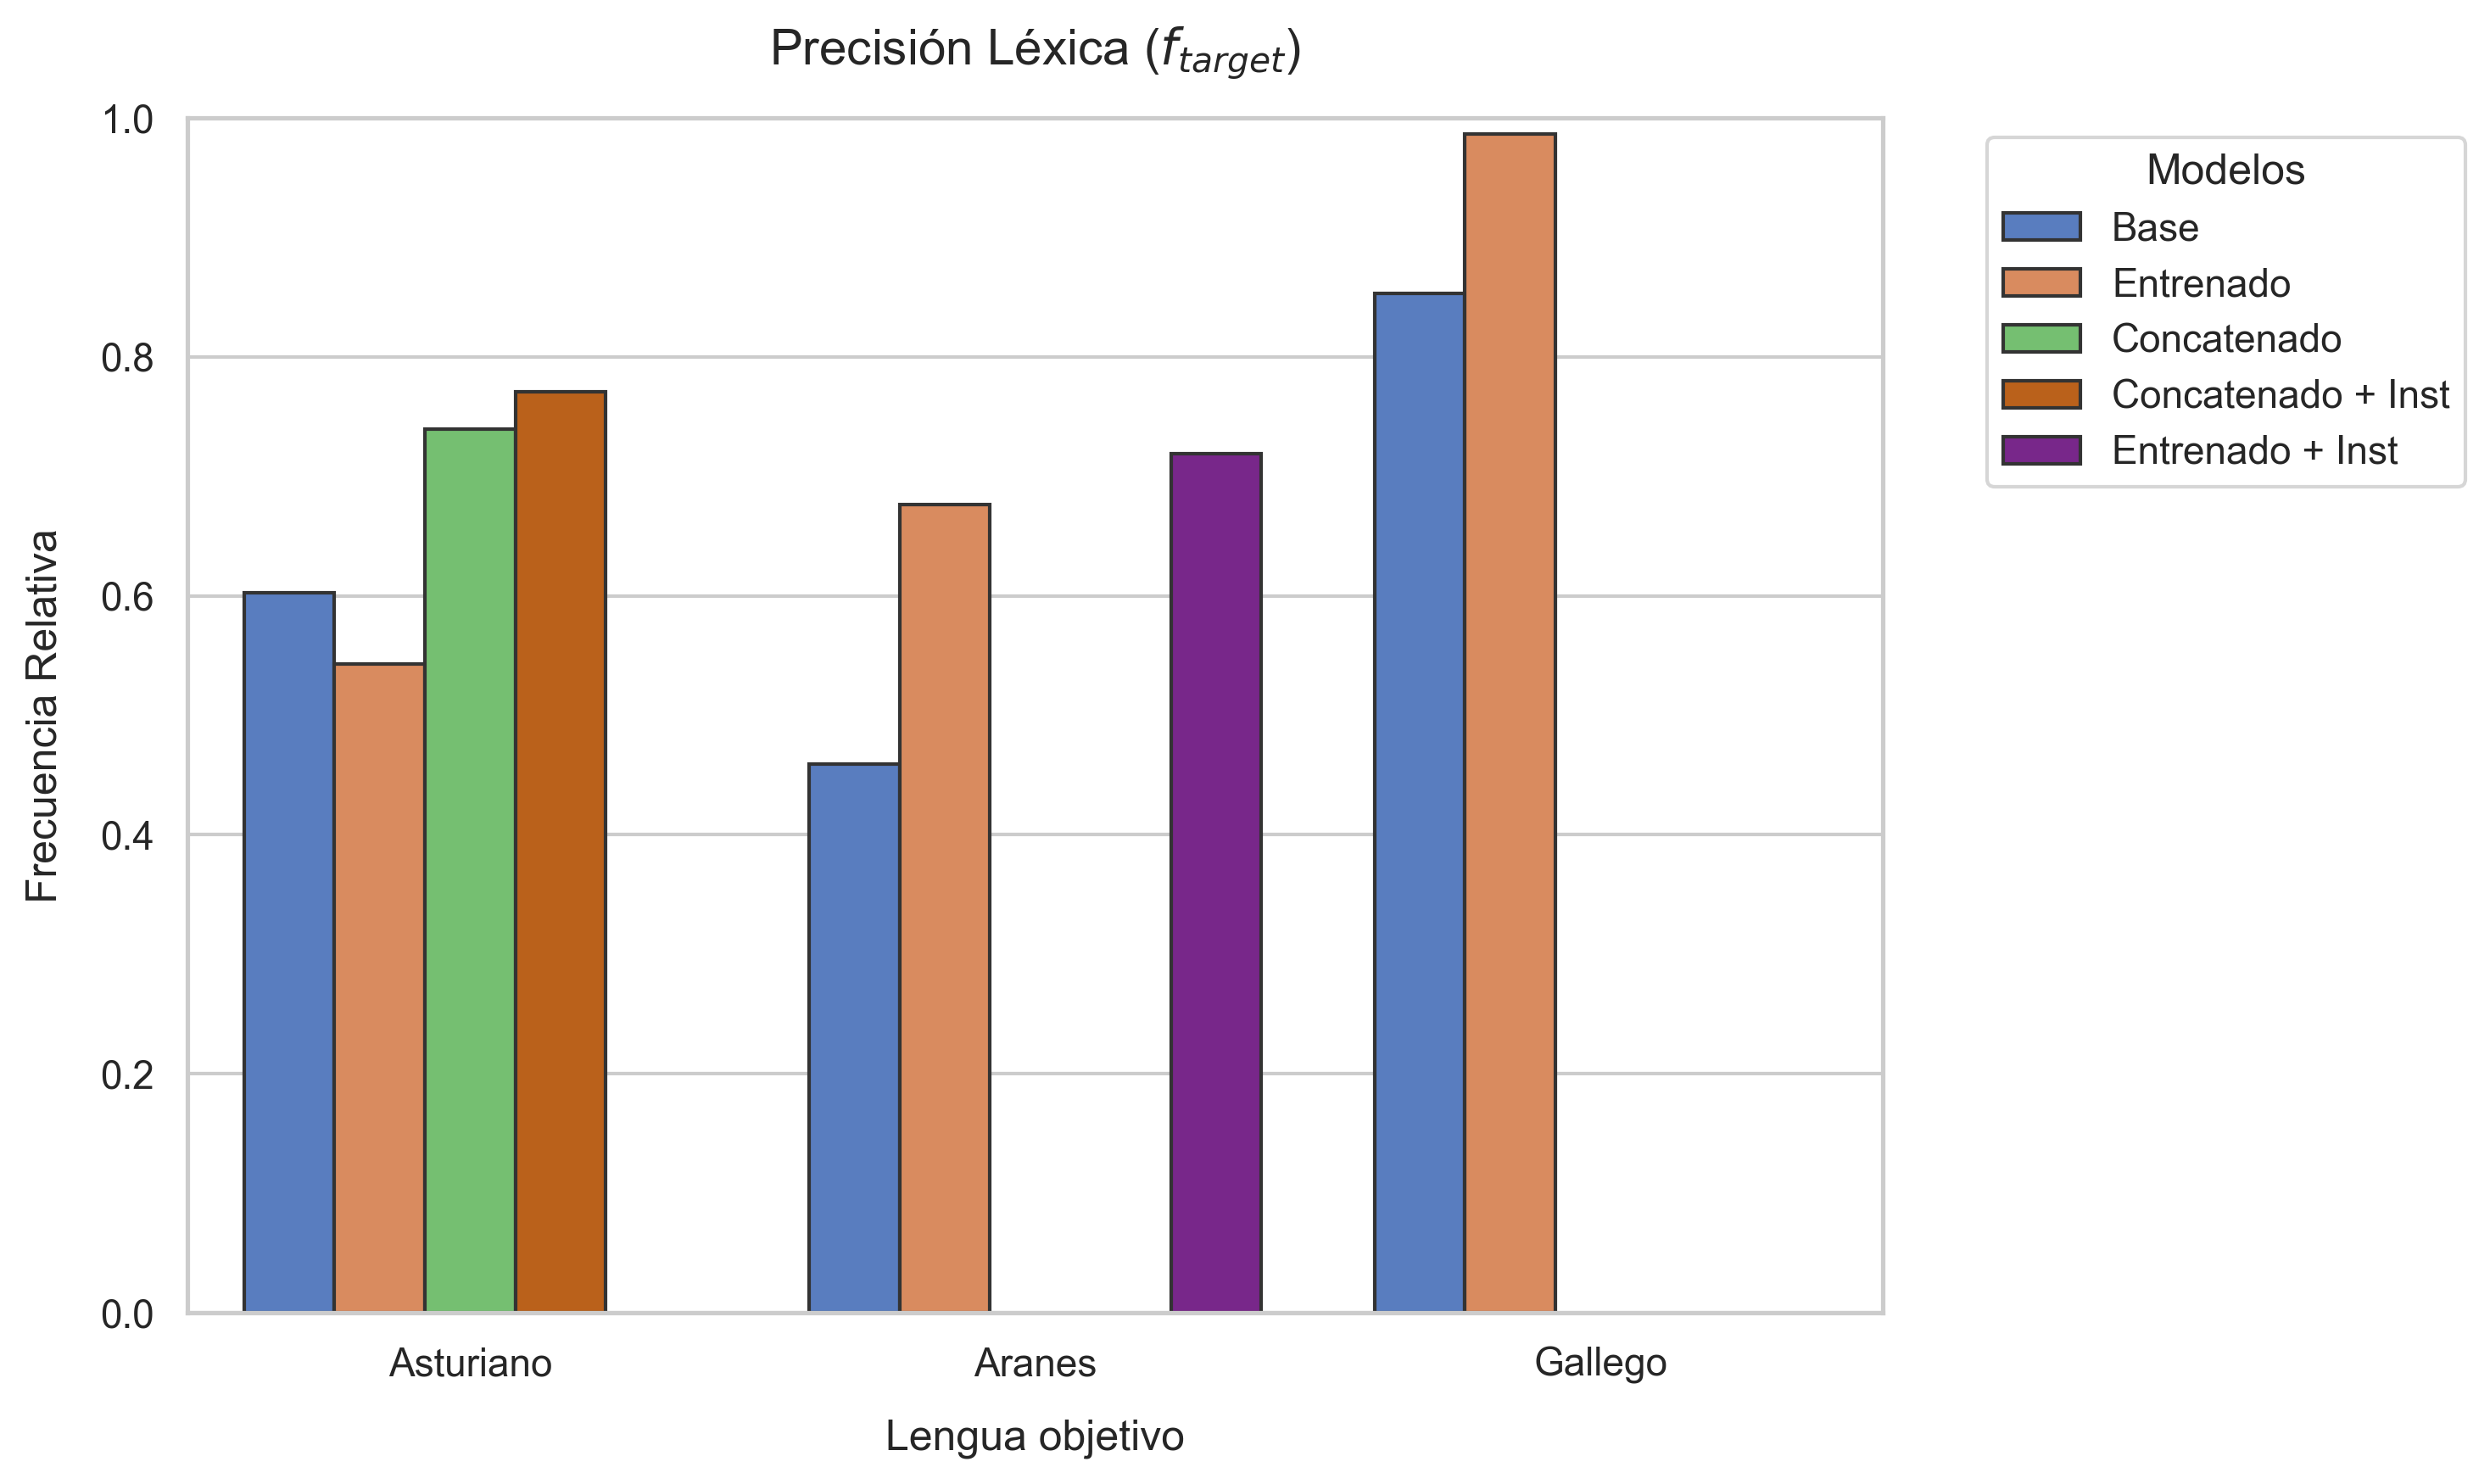
\includegraphics[width=0.8\textwidth]{figures/Calidad_freq_target_qlora.png}    
    \caption{\label{fig:resultados-qlora-freq-target}Freq target de los modelos entrenados por lengua. De creación propia.}
\end{figure}

\textit{En la Figura \ref{fig:resultados-qlora-freq-target} se observa que, en el caso del aranés y del gallego, no se entrenó la versión concatenada debido a la pérdida de coherencia detectada previamente en asturiano. Por tanto, la ausencia de barras en esas lenguas no indica un rendimiento de 0, sino simplemente que esa combinación no fue entrenada.}

En la Figura \ref{fig:resultados-qlora-freq-target} se observa que, en general, todos los modelos entrenados mejoran a sus modelos base en el porcentaje de palabras pertenecientes al diccionario de la lengua objetivo. Destaca especialmente el modelo entrenado en gallego, que pone de manifiesto la importancia de la calidad de los datos: alcanza un 98\% de palabras presentes en el diccionario, una cifra coherente con lo esperable para un modelo que domina la lengua, considerando además posibles ausencias en el diccionario, nombres propios y abreviaturas.
Por otro lado, el modelo entrenado del asturiano es el único que ha bajado de calidad frente a los modelos base.

\begin{figure}[H]
    \centering
    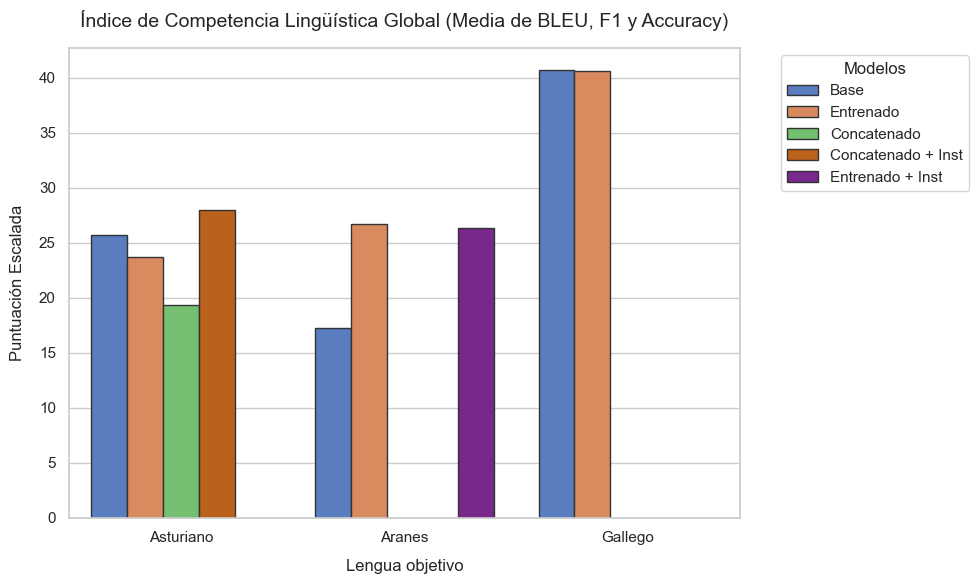
\includegraphics[width=0.8\textwidth]{figures/IndiceMetricas_qlora.png}    
    \caption{\label{fig:resultados-qlora-indice-metricas}Índice global de los resultados de los modelos entrenados por lengua. De creación propia.}
\end{figure}

En la gráfica de media de métricas de evaluación, en la Figura \ref{fig:resultados-qlora-indice-metricas} (calculada como se explicó en \nameref{indice-agrupacion-metricas}) se muestra una mejora de los modelos entrenados, aunque mucho menor, principalmente debido a esa perdida de coherencia. Curiosamente, el modelo que peor funcionaba en el asturiano en freq target, obtiene un mejor resultado que el modelo concatenado en esta métrica, debido a esta perdida de coherencia al concatenar las muestras.

En el gallego, el modelo entrenado mantiene la calidad en este índice, mejorando el número de palabras bien escritas, siendo el mejor resultado del trabajo.

Por último, en el caso del \textit{Aranés}, los resultados muestran mejoras apreciables en ambas métricas, aunque los ejemplos cualitativos revelan que el modelo aún no alcanza un nivel de calidad elevado. Esto sugiere que el modelo base parte de un desempeño especialmente bajo en Aranés, a pesar de la cercanía lingüística con el catalán, y que el entrenamiento consigue una mejora significativa y consistente. Es, de hecho, el caso más llamativo del estudio, es la lengua en la que el modelo más progresa y lo hace de manera más uniforme en ambas gráficas, aunque todavía quede margen para alcanzar una calidad plenamente satisfactoria.

\chapter{Aspectos legales, éticos y sociales e impacto}
\label{ch:analisis}

En los últimos años, el desarrollo de modelos de lenguaje de gran tamaño ha avanzado a un ritmo extraordinario, impulsado por la disponibilidad de grandes corpus textuales y por técnicas de entrenamiento cada vez más eficientes. Sin embargo, el uso de datos lingüísticos, especialmente cuando proceden de lenguas minoritarias, plantea una serie de consideraciones legales, éticas y sociales que deben analizarse con detenimiento. Este capítulo examina estos aspectos en relación con el trabajo realizado adaptando modelos mediante QLoRA para mejorar su competencia en asturiano, aranés y gallego, así como en la creación de un benchmark específico para evaluar su rendimiento.

\section{Aspectos legales, éticos y profesionales}

\subsection{Licencias}

El uso de datos textuales para entrenar y evaluar modelos de lenguaje está condicionado por las licencias de los corpus empleados y por las implicaciones derivadas de la generación automática de contenido. En este trabajo se han utilizado distintos conjuntos de datos públicos, cada uno con su marco legal específico.

Los datos de entrenamiento proceden principalmente de \textbf{OPUS‑NLLB v1}, un corpus multilingüe distribuido bajo licencia \textbf{ODC‑By}. Esta licencia permite el uso, modificación y redistribución de los datos siempre que se mantenga la atribución correspondiente. Para el entrenamiento del modelo en gallego se utilizó el corpus NOS, que incluye subcorpus con licencias heterogéneas, como CC BY‑NC‑ND 4.0, Apache 2.0 o CC0, lo que obliga a respetar las restricciones específicas de cada uno.

El corpus ALIA, empleado para evaluación, se distribuye bajo licencia \textbf{CC BY‑SA 4.0}, que permite reutilización y adaptación siempre que se comparta bajo la misma licencia.

Finalmente, los recursos lingüísticos de FreeLing utilizados para español se encuentran bajo \textbf{AGPL}, una licencia copyleft que permite su uso académico siempre que las modificaciones se distribuyan bajo los mismos términos.

Además de los corpus textuales, este trabajo emplea datos generados por modelos de lenguaje, tanto para la creación de errores controlados como para la evaluación automática. En estos casos, la autoría del contenido generado recae en los modelos utilizados, y su uso es compatible con las licencias de las plataformas empleadas. 
Se han utilizado modelos de IA también para la búsqueda bibliográfica, asistir en la redacción y detección de errores en el código.

Desde una \textbf{perspectiva ética}, el objetivo principal del proyecto es contribuir a la preservación y normalización de lenguas minoritarias mediante la mejora de su representación en modelos de lenguaje. 
Para ello, en primer lugar, promueve la \textbf{justicia lingüística}, al facilitar que comunidades con menos recursos tecnológicos puedan acceder a herramientas avanzadas que normalmente solo están disponibles para lenguas mayoritarias. En segundo lugar, la metodología utilizada, basada en datos abiertos, técnicas eficientes y documentación transparente, favorece la \textbf{investigación responsable}, ya que permite reproducir y auditar el proceso. En tercer lugar, la creación de un benchmark específico para entrenar modelos con pocos datos, contribuyendo a establecer \textbf{estándares de evaluación claros} y reduciendo la opacidad habitual en el desarrollo de modelos de lenguaje y ayuda a detectar sesgos o errores de forma sistemática. 

\textbf{No obstante, el uso de datos lingüísticos puede introducir riesgos significativos}. Los corpus disponibles para lenguas minoritarias suelen ser reducidos y no siempre representativos de la diversidad dialectal, sociolingüística o estilística de la comunidad. Esto puede generar \textbf{sesgos} en los modelos, tales como:
\begin{itemize}
    \item \textbf{Sobrerrepresentación de ciertos registros} (por ejemplo, textos institucionales o literarios) frente al habla cotidiana.
    \item \textbf{Errores en datos de entrenamiento} si el corpus contiene errores o formas no estandarizadas.
    \item \textbf{Reproducción de sesgos ideológicos o culturales} presentes en los textos originales, especialmente en corpus extraídos de internet.
\end{itemize}

Además, la generación automática de contenido plantea el riesgo de que usuarios no expertos tomen como correctas producciones erróneas, lo que podría afectar negativamente a la transmisión intergeneracional de la lengua o a su estandarización.


\subsection{Aspectos profesionales}

En cuanto a los \textbf{aspectos profesionales}, este trabajo se enmarca en un contexto académico y metodológico. No se plantea un uso comercial del modelo, sino la demostración de una metodología reproducible para adaptar LLMs a lenguas minoritarias con recursos limitados. La publicación del benchmark y de los datasets derivados permitirá que otros investigadores puedan replicar, mejorar o ampliar el estudio sin necesidad de repetir todo el proceso desde cero.

\section{Impacto social, económico y medioambiental}

El desarrollo de modelos de lenguaje adaptados a lenguas minoritarias tiene implicaciones que van más allá del ámbito técnico. En esta sección se analizan los principales impactos derivados del proyecto, tanto positivos como potenciales riesgos.

\subsection{Impacto social}

El impacto social más relevante de este trabajo está relacionado con la revitalización lingüística. Las lenguas minoritarias como el asturiano o el aranés presentan un riesgo real de desplazamiento frente al castellano o el francés. Según el \textit{UNESCO Atlas of the World's Languages in Danger} \cite{unesco_atlas_2010}, ambas lenguas se encuentran clasificadas como \textit{definitely endangered}, lo que implica que su transmisión intergeneracional es limitada y que su presencia en ámbitos formales y digitales resulta insuficiente. La falta de presencia tecnológica se considera uno de los factores que pueden acelerar la pérdida de vitalidad lingüística, especialmente en contextos donde la digitalización determina el acceso al conocimiento y la participación cultural.

En este sentido, la disponibilidad de herramientas tecnológicas como correctores, traductores o modelos instructivos puede facilitar el uso cotidiano de estas lenguas y aumentar su presencia en entornos digitales, donde actualmente están infrarrepresentadas. La existencia de recursos digitales es un elemento que contribuye a que una lengua pueda participar en la sociedad del conocimiento y mantener su funcionalidad en ámbitos contemporáneos \cite{unesco_diversity_2003}.

La creación de un benchmark específico contribuye a facilitar su estudio y promueve la generación de nuevos recursos lingüísticos. Esto puede tener un efecto positivo en la disponibilidad de herramientas para estas lenguas y favorecer su mantenimiento a largo plazo. La literatura especializada señala que la ausencia de recursos digitales puede conducir a situaciones de \textit{digital language death}, donde la lengua pierde funcionalidad en los espacios tecnológicos actuales \cite{moseley_2012_digital}. La existencia de datos evaluables y comparables permite mitigar este riesgo y fomenta el desarrollo de sistemas más robustos y culturalmente adecuados.

No obstante, también existen riesgos. Un modelo que genere contenido incorrecto puede reforzar formas no normativas o inducir a error a usuarios no expertos. Además, la automatización excesiva puede desplazar prácticas culturales tradicionales asociadas al uso de la lengua. Documentos recientes sobre ética de la inteligencia artificial señalan la importancia de evitar sesgos que afecten negativamente a comunidades vulnerables y de garantizar que los sistemas respeten la diversidad cultural y lingüística \cite{unesco_ai_2021}. Por ello, estas herramientas deben utilizarse como apoyo y no como sustituto del conocimiento lingüístico humano.

En conjunto, este trabajo contribuye a reducir la brecha tecnológica entre lenguas mayoritarias y minoritarias y puede favorecer la mejora de la vitalidad digital de lenguas en riesgo. Además, proporciona un marco evaluativo que permitirá desarrollar herramientas más precisas, éticas y culturalmente adecuadas.


\subsection{Impacto económico}

Desde el punto de vista económico, este proyecto se caracteriza por su bajo coste. Se han utilizado modelos y datos abiertos, así como plataformas gratuitas como la API de Groq. El único gasto significativo ha sido el uso de máquinas en la nube durante aproximadamente dos meses y medio.

La elección de \textbf{QLoRA} tiene un impacto económico directo: permite entrenar modelos grandes con un consumo de memoria y energía muy reducido en comparación con un reentrenamiento completo. Esto hace que la metodología sea accesible para instituciones educativas, investigadores independientes o comunidades lingüísticas sin grandes infraestructuras computacionales.

Además, la publicación del benchmark y de los datasets derivados puede reducir costes futuros para otros investigadores, al proporcionar una base sólida sobre la que continuar trabajando sin necesidad de reconstruir todo el pipeline.

\subsection{Impacto medioambiental}

El entrenamiento de modelos de lenguaje tiene un coste energético significativo, especialmente cuando se utilizan arquitecturas de gran tamaño. Sin embargo, en este proyecto se ha optado por técnicas que minimizan dicho impacto. La cuantización a 4 bits y la reducción del número de parámetros entrenables mediante QLoRA disminuyen drásticamente el consumo energético respecto a un entrenamiento completo.

Asimismo, el uso de hardware en la nube durante un periodo limitado y la reutilización de modelos preentrenados contribuyen a reducir la huella de carbono asociada al proyecto. Aunque no se dispone de datos exactos sobre el consumo energético de cada entrenamiento, se puede afirmar que el impacto medioambiental es significativamente menor que el de proyectos de entrenamiento desde cero.

Por último, la metodología propuesta puede servir como referencia para futuros trabajos que busquen equilibrar eficiencia computacional y sostenibilidad.

\subsection*{Contribución a los Objetivos de Desarrollo Sostenible (ODS)}

El trabajo desarrollado contribuye de manera directa al \textbf{ODS 10 (Reducción de las desigualdades)}. Las lenguas minoritarias como el asturiano, el aranés o el gallego presentan una clara desventaja en el ámbito tecnológico debido a su escasa presencia en los corpus utilizados para entrenar modelos de lenguaje. La adaptación de LLMs mediante técnicas eficientes como QLoRA y la creación de un benchmark específico para todas las lenguas minoritarias, permiten reducir esta brecha, favoreciendo un acceso más equitativo a herramientas lingüísticas avanzadas y promoviendo la justicia lingüística.

De forma complementaria, el proyecto también se alinea con el \textbf{ODS 4 (Educación de calidad)}, al generar recursos que pueden emplearse en contextos educativos para apoyar la enseñanza y normalización de estas lenguas y con el \textbf{ODS 11 (Ciudades y comunidades sostenibles)}, al contribuir a la preservación del patrimonio cultural inmaterial.

En conjunto, la metodología propuesta impulsa un desarrollo tecnológico más inclusivo y respetuoso con la diversidad lingüística.

\chapter{Conclusiones y trabajo futuro}
\label{ch:analisis}

A lo largo del proyecto se han obtenido avances relevantes en la adaptación de modelos de lenguaje a lenguas minoritarias, así como una comprensión más clara de las limitaciones y desafíos asociados a este proceso. El análisis conjunto del corpus preparado, de los modelos entrenados y del benchmark desarrollado permite identificar mejoras consistentes en la calidad lingüística, al mismo tiempo que pone de manifiesto aspectos que requieren un tratamiento más profundo, como la preservación de la instructividad o la necesidad de datos más amplios y homogéneos. A partir de esta visión global, se presentan a continuación las conclusiones principales y las líneas de trabajo que podrían guiar futuras investigaciones.

\section{Conclusiones}

El trabajo realizado ha permitido avanzar de manera significativa en la adaptación de modelos de lenguaje a lenguas minoritarias como el asturiano, el aranés y el gallego. A partir de un proceso de recopilación, limpieza y normalización de corpus, se ha conseguido disponer de datos más homogéneos y adecuados para el entrenamiento, reduciendo interferencias lingüísticas y problemas derivados de la fragmentación del texto. Pese a una disponibilidad de recursos limitada, el tratamiento aplicado ha demostrado ser suficiente para entrenar modelos estables y evaluar su comportamiento de forma controlada.

La creación de un benchmark específico ha supuesto una contribución relevante, al ofrecer un conjunto de tareas que permiten evaluar modelos en contextos donde no existen datasets estandarizados. Las pruebas de traducción, corrección lingüística y detección de castellanización han permitido medir competencias fundamentales y comparar de manera objetiva tanto modelos base como modelos ajustados. Si bien el benchmark no cubre todavía todas las dimensiones posibles de evaluación, sí proporciona una base sólida y reutilizable para trabajos posteriores.

El entrenamiento mediante QLoRA ha mostrado mejoras claras en corrección morfológica y adecuación lingüística, especialmente cuando se han incorporado estrategias como la concatenación de ejemplos y el uso de datos instructivos. Las limitaciones de hardware han condicionado la longitud máxima de secuencia y el tamaño de los lotes, lo que ha impedido explorar configuraciones más ambiciosas. Aun así, los resultados obtenidos indican que es posible mejorar modelos generales con un coste computacional reducido y con corpus relativamente pequeños.

El principal problema que se ha encontrado al entrenar es la pérdida del caracter instructivo del modelo, convirtiendose en un modelo que genera texto, pero le cuesta contestar preguntas. Conseguir adaptarlo después o entrenarlo sin perder esa característica sería un estudio de ampliación de este TFG muy interesante.

La comparación entre el modelo antes y después del ajuste fino confirma que el entrenamiento específico por lengua produce avances medibles, aunque no uniformes en todas las tareas. En particular, se observa una reducción consistente de la interferencia con el castellano y una mayor estabilidad en la generación, mientras que aspectos más complejos, como la producción de textos largos o altamente especializados, siguen mostrando limitaciones propias del tamaño del modelo y del volumen de datos disponibles.

Finalmente, el trabajo ha permitido establecer una metodología reproducible que abarca desde la preparación del corpus hasta la evaluación final. Esta metodología, junto con el benchmark y los análisis realizados, constituye un marco de referencia útil para futuras investigaciones orientadas a mejorar el tratamiento automático de lenguas minoritarias. Aunque no todos los aspectos han podido desarrollarse con la profundidad deseada, los resultados obtenidos muestran que es posible avanzar de forma rigurosa y sistemática incluso en escenarios de recursos escasos, y sientan las bases para continuar ampliando la cobertura lingüística y la calidad de los modelos en este ámbito.

Este trabajo demuestra que es posible adaptar LLMs modernos a lenguas minoritarias con recursos extremadamente limitados, y establece un marco reproducible que puede servir como base para futuros desarrollos en preservación lingüística mediante IA.

\section{Trabajo futuro}

De cara a continuar este trabajo, existen varias líneas de mejora que permitirían obtener modelos más robustos y evaluaciones más fiables. En primer lugar, sería deseable repetir la metodología con una mayor capacidad de cómputo, lo que permitiría entrenar con secuencias más largas, tamaños de lote mayores y configuraciones de QLoRA más amplias. Esto abriría la puerta a explorar modelos más pequeños pero entrenados durante más tiempo, así como a estudiar el impacto del tamaño del adaptador en la calidad final del modelo.

Otra línea de mejora se encuentra en el propio \textit{benchmark}. Actualmente, la selección automática de la respuesta correcta puede resultar imprecisa en tareas como la traducción, donde el modelo a veces ofrece la solución en una frase posterior. Sería conveniente desarrollar un sistema más robusto de extracción de la respuesta, por ejemplo mediante un modelo ligero encargado de eliminar explicaciones y conservar únicamente la salida final, o mediante técnicas basadas en \textit{regex} y medidas de similaridad semántica. Esto aumentaría la fiabilidad del marco de evaluación.

También sería importante mejorar la calidad y representatividad de los datos de entrenamiento en cada lengua, especialmente en aquellas con menos recursos. Un corpus más amplio, equilibrado y limpio permitiría reducir interferencias y mejorar la estabilidad del entrenamiento.

En cuanto al diseño de los \textit{prompts} del benchmark, sería útil ajustarlos para fomentar una mayor obediencia y reducir la tendencia del modelo a desviarse hacia explicaciones innecesarias. Asimismo, convendría penalizar explícitamente las respuestas vacías o incompletas, dado que se han observado con cierta frecuencia.

Finalmente, uno de los retos más relevantes identificados es la pérdida de la capacidad instructiva del modelo tras el ajuste fino. Investigar estrategias para preservar dicha instructividad, o para recuperarla posteriormente mediante técnicas adicionales de \textit{alignment} o \textit{instruction tuning}, constituye una línea de trabajo especialmente prometedora, aunque probablemente requiera recursos computacionales superiores a los disponibles en este TFG.





\endgroup
\printbibliography

% \appendix

% \input{appendices/escuelas-y-titulos}

\printglossary

\end{document}
